%%%%%%%%%%%%%%%%%%%%%%%%%%%%%%%%%%%%%%%%%%%%%
%%%
%%%	MSEE THESIS MASTER DOCUMENT
%%%
%%%%%%%%%%%%%%%%%%%%%%%%%%%%%%%%%%%%%%%%%%%%%

%%%%%%%%%%%%%%%%%%%%%%%%%%%%%%%%%%%%%%%%%%%%%
%%% PREAMBLE

\documentclass[12pt,letterpaper]{report}
\usepackage{UNLV_ECE}
\usepackage{psfrag,graphicx,epsfig,array}
\usepackage{amsmath,amsfonts,amssymb,amsthm,amsxtra}
\usepackage{bm}
\usepackage{multirow,booktabs}
\usepackage{caption}
\usepackage{checkend}
\usepackage{hyperref}
\usepackage{cite}
\usepackage{rotating}
\usepackage{float}
\notocheads
\logicalnumbering
% \usepackage{layout}

\usepackage[T1]{fontenc}
\usepackage{lmodern}

\doublespace

%%%%%%%%%%%%%%%%%%%%%%%%%%%%%%%%%%%%%%%%%%%%%
%%% FUNCTIONS

\newcommand{\CTDSM}		{Continuous-Time $\Delta\Sigma$ Modulator }
\newcommand{\DTDSM}		{Discrete-Time $\Delta\Sigma$ Modulator }
\newcommand{\CTDSMs}	{Continuous-Time $\Delta\Sigma$ Modulators }
\newcommand{\DTDSMs}	{Discrete-Time $\Delta\Sigma$ Modulators }
\newcommand{\DSM}		{$\Delta\Sigma$ Modulator }
\newcommand{\DSMs}		{$\Delta\Sigma$ Modulators }
\newcommand{\DSm}		{$\Delta\Sigma$ modulator }
\newcommand{\DSms}		{$\Delta\Sigma$ modulators }
\newcommand{\DS}		{$\Delta\Sigma$\space}
\newcommand{\CT}		{Continuous-Time }
\newcommand{\DT}		{Discrete-Time }
\newcommand{\ct}		{continuous-time }
\newcommand{\dt}		{discrete-time }
\newcommand{\ntf}		{noise transfer function }
\newcommand{\stf}		{signal transfer function }
\newcommand{\wrt}		{with respect to }
\newcommand{\nth}		{$n$th}
\newcommand{\ith}		{$i$th}
\newcommand{\mc}[3]		{\multicolumn{#1}{#2}{#3}}
\newcommand{\mr}[2]		{\multirow{#1}*{#2}}
\newcommand{\norm}[1]	{\lVert#1\rVert}
\newcommand{\abs}[1]	{\lvert#1\rvert}
\newcommand{\fix}[1] 	{\texorpdfstring{#1}}
\newcommand{\NTF}		{\mathop\text{NTF}}
\newcommand{\STF}		{\mathop\text{STF}}

\makeatletter
\newcommand*\dashline{\rotatebox[origin=c]{90}{$\dabar@\dabar@\dabar@$}}
\makeatother

%%%%%%%%%%%%%%%%%%%%%%%%%%%%%%%%%%%%%%%%%%%%%
%%% DOCUMENT BODY
\begin{document}

\mastersthesis
\renewcommand{\thesisauthor}		{Matthew Edward Jackson}
\renewcommand{\thesismonth}			{June}
\renewcommand{\thesisdefensemonth}	{June}
\renewcommand{\thesisyear}			{2009}
\renewcommand{\thesistitle}
{Optimal Design of Discrete-Time \\ Delta Sigma Modulators}
\renewcommand{\thesissupervisor}	{Peter Allen Stubberud}
\renewcommand{\thesistype}			{thesis}
\renewcommand{\thesisdegree}		{Master of Science}
\renewcommand{\thesisdedication}	{To my dog.}
\renewcommand{\thesisfrontheadsize}	{\normalsize}

% FRONT MATTER
\thesistitlepage
\thesiscopyrightpage
\thesissignaturepage

% ABSTRACT
\newpage
\addcontentsline{toc}{chapter}{ABSTRACT}
\begin{thesisabstract}
150 words go here.
\end{thesisabstract}

\tableofcontents
\listoffigures
\listoftables

% ACKNOWLEDGMENTS
\newpage
\addcontentsline{toc}{chapter}{ACKNOWLEDGMENTS} 
\begin{thesisacknowledgments}
Nice things go here.
\end{thesisacknowledgments}

% CHAPTER 1: INTRODUCTION
\chapter{Introduction}
\label{ch:Introduction}
%%%%%%%%%%%%%%%%%%%%%%%%%%%%%%%%%%%%%%%%%%%%%
%
%  CHAPTER 1: Introduction
%
%%%%%%%%%%%%%%%%%%%%%%%%%%%%%%%%%%%%%%%%%%%%%

Mixed-signal systems are systems that possess both analog and digital subsystems. Such
systems are prevalent in test and measurement platforms, data acquisition systems, and
communications devices. Thus, these mixed-signal systems are often central to hardware
applications ranging from common consumer products such as cellular telephones to highly
specialized real-time data collection systems used in mission critical applications such
as space flight.

In mixed-signal systems, the conversion from analog to digital is performed by
an analog-to-digital converter (ADC). Conversely, the conversion from
digital to analog is performed by a digital-to-analog converter (DAC).
These devices are mixed-signal devices that allow for the
ebb and flow of information between the analog world and digital or discrete-time systems
which are now prevalent throughout electrical applications. Because the performance of
digital systems can usually be improved by simple hardware or software changes, the
performance of a mixed-signal system is often limited by the performance of its data
converters.  As a result, the performance of many mixed-signal systems can be improved by
improving the system's data converter performance.

Many different ADC architectures exist and each architecture has its own benefits and
limitations. \DS modulators are an ADC architecture that uses relatively simple analog
circuitry including a low order quantizer and a feedback loop to sample analog signals
with high signal to noise ratios (SNRs) and large dynamic ranges (DRs).  
Because of the simplicity of the architecture, \DS modulators lend themselves to being
implemented in CMOS process technologies which offer mixed-signal electronics, low-power
performance and high levels of integration \cite{kester_analog_2006}.

\DS modulators achieve high SNRs and large DRs by using a feedback loop
filter to attenuate the quantizer's noise in the frequency bands of interest while passing
the input signal to the output. The transfer function describing the loop filter that
attenuates the quantizer's noise is referred to as the $\Delta\Sigma$'s noise transfer
function (NTF). Similarly, the transfer function describing the loop filter that passes
the input signal to the output is called the signal transfer function (STF).  For lowpass
\DS modulators, the NTF is designed as a high-pass filter so that the noise energy is
attenuated within the low-frequency signal band. Conversely, the STF is designed as a
lowpass filter so that the input signals within the low-frequency signal band are not
attenuated. The STF can also act as an anti-aliasing filter. Thus, the output of a \DS
modulator can be modeled as the sum of an input signal filtered by a STF and a noise
source filtered by a NTF.

In this thesis, optimal signal transfer functions (STFs) and noise transfer functions
(NTFs) for \DS modulators are determined using a novel hybrid orthogonal genetic (HOG)
algorithm. For a given oversampling rate (OSR), which is loosely defined as the
ratio of the $\Delta\Sigma$'s sampling frequency to the input signal's Nyquist frequency,
the $\Delta\Sigma$'s STF and NTF are optimized with respect to a weighted combination of
the \DS modulator's signal-to-noise ratio (SNR) and dynamic range (DR).

% CHAPTER 2: BACKGROUND
\chapter{Analog-to-Digital Converters and $\Delta\Sigma$ Modulators}
\label{ch:ADCs and DSMs}
%%%%%%%%%%%%%%%%%%%%%%%%%%%%%%%%%%%%%%%%%%%%%%%%
%
%  CHAPTER 2: Analog-to-Digital Converters and DSMs
%
%%%%%%%%%%%%%%%%%%%%%%%%%%%%%%%%%%%%%%%%%%%%%%%%

%%%%%%%%%%%%%%%%%%%%%%%%%%%%%%%%%%%%%%%%%%%%%%%%
%%% Section 2.1 - Introduction
%%%%%%%%%%%%%%%%%%%%%%%%%%%%%%%%%%%%%%%%%%%%%%%%
% \section{Introduction}
Analog-to-digital converters (ADCs) are systems which convert continuous-time, continuous
amplitude, or analog, signals into discrete-time, discrete amplitude, or digital signals.
Typically, an ADC converts an analog signal, $x_a(t)$, defined over a continuous finite
interval, $R$, into a digital signal, $x(n)$, defined over a discrete number, $L$, of
values which span the interval $R$. The number, $L$, of discrete values that an ADC can
produce is referred to as the ADC's resolution. Because most ADCs interface with binary
electronic systems, an ADC's resolution is typically a power of 2; that is, $L=2^B$ where
$B$ is an integer representing the binary bit-width of the ADC interface. Thus, ADC
resolution is often expressed in terms of the number, $B$, of bits and not the number,
$L$, of available quantization levels.

\sloppy
For linear ADCs, each of the $2^B$ quantization levels are equidistant over the signal
span $R$. For such ADCs, the quantization step size, $\Delta$, or distance between
adjacent quantization levels is expressed as $\Delta=R/2^B$ where $R$ corresponds to the
input signal span as defined above. For example, consider an analog input, $x_a(t)$, which
has a signal span from -1 to 1; that is, consider an analog input, $x_a(t)$, where
$$-1\leq
x_a(t) \leq 1$$ which has a signal span, $R$, where $R=2$. For a 2-bit system, the signal
span, $R$, is divided into $2^2$ equidistant levels where the quantization step size,
$\Delta$, is $$\Delta=\frac{R}{2^B}=\frac{2}{2^2}=0.5\text{.}$$ This example is
illustrated in Figure \ref{fig:2_bit_quant} for $x_a(t)=\cos(2\pi 1000 t)$, $x_a(n
T_s)=\cos(\pi n/32)$ for $T_s=1/64\pi 1000$, and $x(n)=\mathcal{Q}\left[x_a(n
T_s)\right]$ where $T_s$ is the sampling period in time per sample and 
$\mathcal{Q}[\cdot]$ is the transformation that quantizes the continuous amplitude,
discrete-time signal, $x_a(nT_s)$, by rounding the amplitude to the nearest quantization
level.
%-------------------
\begin{figure}[htbp]
 \centering
 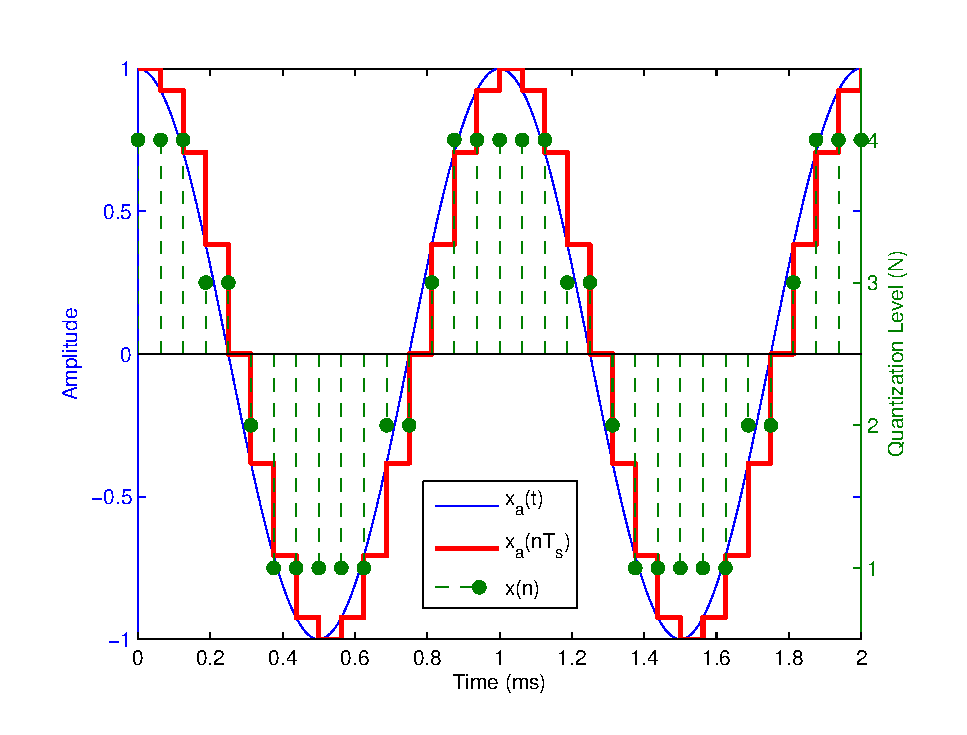
\includegraphics[width=0.8\textwidth]{./matlab_figures/2_bit_intro}
 \caption{2-Bit Quantization}
 \label{fig:2_bit_quant}
\end{figure}
%-------------------

The difference, $x_a(n T_s)-x(n)$, is commonly referred to as the quantization error and
is often characterized as quantization noise in the ADC's output. As shown in Figure
\ref{fig:2_bit_quant}, the digital signal, $x(n)$, is different than both the
analog input signal, $x_a(t)$, and the discrete-time, continuous amplitude signal, 
$x_a(n T_s)$. As the number, $B$, of bits increases, the quantization error, or 
quantization noise, typically decreases. Thus, an ADC's quantization noise is typically a
function of the number, $B$, of quantization bits. In practice, however, ADC levels are
not equally spaced; that is, $\Delta$ varies slightly over the interval $R$. This
non-uniformity in level spacing creates distortion which is also often characterized as
noise in the ADC output. Non-uniform level spacing along with other non-idealities such as
improper input signal conditioning, system thermal noise, and sample clock jitter, limit
an ADC's effective resolution to less than the ideal. As a result, an ADC's effective
resolution is often determined from the ADC's output signal-to-noise ratio (SNR) or
dynamic range (DR) which are performance metrics that are  independent of the ADC's native
architecture.

SNR is defined as the ratio of output signal power to output noise power which contains
power from quantization error and other ADC non-idealities. Dynamic range is defined as
the ratio of the maximum to the minimum detectable signal levels. DR differs from SNR when
the noise floor is not perfectly flat; i.e., noise power in localized frequency regions is
greater than the average noise power. The effects of DR further limit the practical
performance of ADCs. As such, an ADC's effective resolution is often calculated from
the ADC's SNR and DR. The effective resolution is referred to as the ADC's effective
number of bits (ENOB) where ENOB is defined as the achievable ADC resolution when its
non-ideal ADC characteristics are considered.

$\Delta\Sigma$ modulators are ADCs which achieve high SNRs and large DRs by using a
feedback loop filter to attenuate the quantization noise in the frequency band of
interest while passing the input signal to the output. The transfer function describing
the loop filter that attenuates the quantization noise is referred to as the noise
transfer function (NTF). Similarly, the transfer function describing the loop filter that
passes the input signal to the output is referred to as the signal transfer function
(STF).  For example, the NTF for lowpass $\Delta\Sigma$ modulators is designed as a
highpass filter so that the noise energy is attenuated within the low-frequency signal
band. The STF for lowpass $\Delta\Sigma$ modulators is designed as a lowpass
filter so that the input signals within the low-frequency signal band are not attenuated.
In addition, the lowpass characteristics of the STF can also act as an anti-aliasing
filter. As such, the output of a lowpass $\Delta\Sigma$ modulator can be modeled as the
sum of a noise source that is highpass filtered by the NTF and an input signal that is
lowpass filtered by the STF.

 $\Delta\Sigma$ modulator NTFs and STFs are typically designed and implemented  as either
discrete or analog linear recursive filters. As such, a $\Delta\Sigma$ modulator's NTF and
STF can be designed using traditional filters such as Chebyshev or Butterworth filters.
However, these methods are not easily adaptable to the atypical frequency response
characteristics commonly required by many $\Delta\Sigma$ modulators. Historically,
numerical optimization methods have been applied to the optimal design of linear recursive
filters with good success
\cite{rabiner_linear_1974}\cite{chen_design_1990}\cite{cortelazzo_simultaneous_1984}. As
such, design techniques which rely heavily on numerical optimization methods can be used
to optimize $\Delta\Sigma$ modulator system design. Some numerical filter design
programs include other electronic design automation (EDA) tools which automate much of the
design process. For example, the Delta Sigma Toolbox for
MATLAB\textsuperscript{\textregistered} provides an integrated set of discrete-time
$\Delta\Sigma$ modulator design, simulation, and synthesis utilities
\cite{schreier_understanding_2004}. However, this thesis will show that the design method
in the Delta Sigma toolbox offers only marginal improvement over traditional Chebyshev or
Butterworth polynomial based filter design methods.

In this thesis, a global numerical optimization algorithm, called the hybrid orthogonal
genetic (HOG) algorithm, is developed which can determine the optimal design of both
discrete and analog linear recursive filters. In this thesis, the HOG algorithm is used to
optimize the performance of $\Delta\Sigma$ modulator's NTFs and STFs by maximizing
the in-band SNR and DR.

%%%%%%%%%%%%%%%%%%%%%%%%%%%%%%%%%%%%%%%%%%%%%%%%
%%% Section 2.2 - ADC Operational Theory
%%%%%%%%%%%%%%%%%%%%%%%%%%%%%%%%%%%%%%%%%%%%%%%%
\section{Operational Theory}
Figure \ref{fig:basic_adc} shows a basic mathematical model of an ADC. As illustrated,
ADCs can be modeled as a sample-and-hold (S/H) circuit in series with a quantizer and
binary encoder. The sample-and-hold circuit samples the analog input signal at discrete
times where the sample-and-hold process is defined as the process of capturing  the
input signal's amplitude at the sample times, $n T_s$, where $n\in I$, and holding it over
the sampling period, $T_s$. The quantizer then approximates the sampled signal's
amplitude, $x_a(n T_s)$, by converting it to one of the ADC's $L$ quantization levels
which are uniformly spaced by the distance $\Delta$ for a linear ADC. Finally, the
binary encoder converts the digital signal, $x(n)$, into a $B$-bit binary code word.
%-------------------
\begin{figure}[htbp]
 \centering
 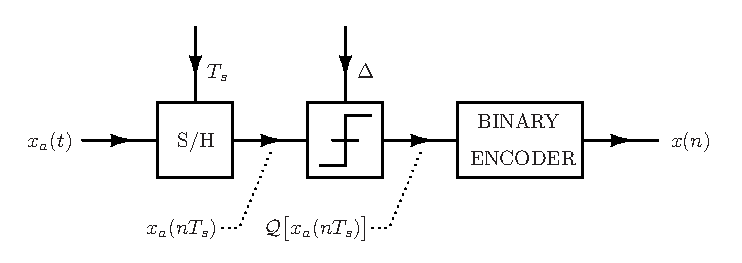
\includegraphics{./final_figures/basic_ADC.eps}
 \caption{Basic ADC Block Diagram}
 \label{fig:basic_adc}
\end{figure}
%-------------------

%%%%%%%%%%%%%%%%%%%%%%%%%%%%%%%%%%%%%%%%%%%%%%%%
%%% 2.2.1: Sampling
%%%%%%%%%%%%%%%%%%%%%%%%%%%%%%%%%%%%%%%%%%%%%%%%
\subsection{Sampling}
The Shannon-Nyquist sampling theorem states that an analog signal must be sampled at a
rate that is at least twice its bandwidth for the analog signal to be reconstructed from
its samples. Specifically, the Shannon-Nyquist sampling theorem states that if an analog
signal, $x_{a}(t)$, is strictly bandlimited such that its Fourier transform, $X_a(f)$, has
the property that $$X_{a}(f) = 0 \quad\lvert f\lvert > f_{0}\text{,}$$ where $f$ is the
instantaneous frequency in cycles per second or Hertz (Hz) and $f_0$ is a fixed frequency,
then $x_a(t)$ can be recovered from its samples, $x_a(n T_s)$, if 
%---------------
\begin{equation}\label{eq:nyquist}
 T_s\leq\frac{1}{2f_{0}}
\end{equation}
%---------------
where $T_s$ is the sampling period in time per sample. The frequency, $f_0$, is referred
to as the Nyquist frequency and the frequency, $2f_{0}$, is referred to as the Nyquist
rate. Converters which sample the input at or near $2f_0$ samples per second  are referred
to as Nyquist rate converters. Common Nyquist rate converter architectures include flash,
dual-slope, successive approximation (SAR), and pipelined converters
\cite{wikipedia_contributors_analog-to-digital_2007}.


%%%%%%%%%%%%%%%%%%%%%%%%%%%%%%%%%%%%%%%%%%%%
%%% 2.2.2 Quantization
%%%%%%%%%%%%%%%%%%%%%%%%%%%%%%%%%%%%%%%%%%%%
\subsection{Quantization}
In this thesis, the quantization transformation, denoted $\mathcal{Q}[\cdot]$, is a
nonlinear transformation which approximates a discrete-time, continuous amplitude
signal by a digital signal that has a finite number of fixed quantization levels. To
illustrate, consider an analog signal, $x_a(t)$, and its corresponding quantized 
signal $x(n)$ where $x(n)=\mathcal{Q}\left[x_a(nT_s)\right]$. If $x(n)$ is a
$B$-bit quantized signal, then the number of quantization
levels, $L$, can be expressed as
%---------------
\begin{equation}\label{eq:quantization_bits}
 L=2^B\text{.}
\end{equation}
%---------------
If the quantized signal, $x(n)$, is bounded such that
%---------------
\begin{equation}\label{eq:quant_magnitude}
\bigl|x(n)\bigr|\leq X_m
\end{equation}
%---------------
where $X_m$ represents the quantizer's maximum input amplitude without saturation, the
quantization interval or step size, $\Delta$, defined as the distance between any two
adjacent quantization levels, can then be expressed as 
%---------------
\begin{equation}\label{eq:quantization_delta}
 \Delta=\frac{X_m}{2^{B-1}}\text{.}
\end{equation}
%---------------

The difference between the discrete-time, continuous amplitude signal, $x_a(nT_s)$,
and the digital signal, $x(n)$, is referred to as the quantization error, $e(n)$. As such,
the quantizer's output, $x(n)$, can be expressed as the sum of the sampled analog
signal, $x_a(n T_s)$, and the quantization error, $e(n)$; that is,
%---------------
\begin{equation}\label{eq:quantizer_output}
x(n)=\mathcal{Q}\bigl[x_a(n T_s)\bigr]=x_a(n T_s)+e(n)
\end{equation}
%---------------
where $\mathcal{Q}[\cdot] $ represents the nonlinear quantization transformation. If a
rounding
quantizer is implemented and it is assumed that:
%---------------
\begin{itemize}
 \item $e(n)$ is a stationary random process
 \item $e(n)$ is uncorrelated with the quantizer's input
 \item $e(n)$ is a white noise process; i.e. it's samples are uncorrelated
 \item $e(n)$ has a probability density that is uniform over the quantization
error range $\bigl[-\Delta/2,\Delta/2\bigr]$
\end{itemize}
%---------------
then the quantizer shown in Figure \ref{fig:linear_quantizer_model}(a) can be modeled by
the linear system shown in Figure \ref{fig:linear_quantizer_model}(b)\cite{
gray_quantization_1990}\cite{ oppenheim_discrete-time_1999}. Using this linear
quantizer model greatly reduces the complexity associated with ADC analysis at the expense
of modeling accuracy. However, it has been shown that for rapidly varying input signals
and small quantization intervals or $\Delta$'s, the results obtained from this linear
noise model are sufficient for most
calculations\cite{oppenheim_discrete-time_1999}\cite{hayes_schaums_1998}.
%-------------------
\begin{figure}[htbp]
 \centering
 \includegraphics*[clip,viewport=0 0 330
150]{./final_figures/linear_quantizer_model.eps}
 \captionsetup{justification=centering} 
 \caption[]{Linear Quantizer Model\\(a) Nonlinear Quantizer (b) Linear
Quantizer Model}
 \label{fig:linear_quantizer_model}
\end{figure}
%-------------------

%%%%%%%%%%%%%%%%%%%%%%%%%%%%%%%%%%%%%%%%%%%%
%%% 2.3 ADC Performance Metrics
%%%%%%%%%%%%%%%%%%%%%%%%%%%%%%%%%%%%%%%%%%%%
\section{Performance Metrics}
An ADC's performance is often described in terms of SNR and DR where both
metrics compare the relative output signal power to the output noise power. Because
deterministic signals and stochastic noise are modeled differently, their respective
powers are calculated using different techniques. For deterministic signals,
power is calculated analytically from the available signal information. For stochastic
signals, power is calculated in terms of the statistical characteristics which define the
signal.

%%%%%%%%%%%%%%%%%%%%%%%%%%%%%%%%%%%%%%%%%%%%%%%%
%%% 2.3.1: Signal and Noise Power
%%%%%%%%%%%%%%%%%%%%%%%%%%%%%%%%%%%%%%%%%%%%%%%%
\subsection{Signal and Noise Power}
The mean or expectation of a continuous random process, $x(t)$, is defined as
 %----------------------
\begin{equation}\label{eq:cont_ensemble_average}
 E\bigl[x(t)\bigr] = \int_{-\infty}^{\infty}{x(t) p_x\bigl(x\left(t\right)\bigr)dx(t)}
\end{equation}
%----------------------
where $p_x\bigl(x\left(t\right)\bigr)$ is the probability density function of $x(t)$.
Similarly, the mean or expectation of a discrete random process, $x(n)$, is defined as
 %----------------------
\begin{equation}\label{eq:discrete_ensemble_average}
 E\bigl[x(n)\bigr] = \sum_{k=1}^{N}{x_k(n)P_{x_k(n)}\bigl(x_k(n)\bigr)}
\end{equation}
%----------------------
where $\{x_k(n): k=1,\cdots,N\}$ is the range of $x(n)$, and
$P_{x_k(n)}\bigl(x_k(n)\bigr)$ is the probability mass function of $x(n)$. Equations
\eqref{eq:cont_ensemble_average} and \eqref{eq:discrete_ensemble_average} are
referred to as the ensemble or state averages of a random process.

The variance, $\sigma_x^2$, of a random process, $x$, is defined as
 %----------------------
\begin{equation}\label{eq:variance}
\sigma_x^2=E\Bigl[\bigl(x-E[x]\bigr)^2\Bigr]
\end{equation}
%----------------------
which can be expressed as 
 %----------------------
\begin{equation}\label{eq:expectation_proof}
\begin{split}
\sigma_x^2& =E\Bigl[\bigl(x-E[x]\bigr)^2\Bigr]\\
& = E\bigl[x^2 - 2xE[x]+E^2[x]\bigr]\\
& = E\left[x^2\right] - E^2[x]\text{.}
\end{split}
\end{equation}
%----------------------
For a zero mean random process, \eqref{eq:expectation_proof} reduces to
 %----------------------
\begin{equation}\label{eq:zero_mean_variance}
\sigma_x^2=E\left[x^2\right]\text{.}
\end{equation}
%----------------------

Calculating the expectation or variance of a random process requires its probability
density or probability mass function. In practice, the probability densities or
probability mass functions for the random variables of a random process are not
necessarily well defined. However, if a random process is said to be ergodic, then the
random process' ensemble average is equivalent to
its time average, and time averages can be used to estimate the random process' mean and
variance\cite{papoulis_probability_1984}\cite{lathi_modern_1998}.

For a continuous-time random process, $x(t)$, the time average, $\mu_{x(t)}$, of $x(t)$ is
defined as 
%----------------------
\begin{equation}\label{eq:cont_time_average}
 \mu_{x(t)}=\displaystyle\lim_{T \to \infty}{\frac{1}{2T}}\int_{-T}^{T}{x(\tau)d\tau}.
\end{equation}
%----------------------
Similarly, for a discrete-time random process, $x(n)$, the time average, $\mu_{x(n)}$,
of $x(n)$ is defined as 
%----------------------
\begin{equation}\label{eq:discrete_time_average}
 \mu_{x(n)}=\displaystyle\lim_{N \to \infty}{\frac{1}{2N+1}}\sum_{k=-N}^{N}{x(k)}.
\end{equation}
%----------------------

Thus, if a zero mean, continuous-time  random process, $x(t)$, is ergodic, the variance,
$\sigma_{x(t)}^2$, of $x(t)$ can be represented in terms of its time average,
$\mu_{x^2(t)}$, as
 %----------------------
\begin{equation}\label{eq:cont_time_variance}
\sigma_{x(t)}^2=E\left[x^2(t)\right]=\mu_{x^2(t)}=\lim_{T \to \infty}
\frac{1}{2T}\int_{-T}^{T}{x^2(\tau)d\tau}\text{.}
\end{equation}
%----------------------
Similarly, if a zero mean, discrete-time random process, $x(n)$, is ergodic, the variance,
$\sigma^2_{x(n)}$, of $x(n)$ can be represented in terms of its time average,
$\mu_{x^2(t)}$, as
 %----------------------
\begin{equation}\label{eq:discrete_time_variance}
\sigma^2_{x(n)}=E\left[x^2(n)\right]=\mu_{x^2(t)}=\lim_{N \to \infty}
\frac{1}{2N+1}\sum_{k=-N}^{N}{x^2(k)}\text{.}
\end{equation}
%----------------------

The power, $P_{x(n)}$, for a deterministic discrete-time signal, $x(n)$, can be calculated
as
%----------------------
\begin{equation}\label{eq:signal_power}
P_{x(n)} =\lim_{N \to
\infty}\frac{1}{2N+1}\sum_{k=-\infty}^{\infty}{x^2(k)}
\end{equation}
%----------------------
which is identical to \eqref{eq:discrete_time_variance}. Therefore, for a zero mean
random signal, $x(n)$, $P_{x(n)}=\sigma^2_{x(n)}$. In practice, SNR and DR are estimated
using
a finite length sequence. Thus, for a signal of length $2N+1$, the average signal
power, $P_{x(n)[-N,N]}$, is
given as
%----------------------
\begin{equation}\label{eq:average_signal_power}
 P_{x(n)[-N,N]} =\frac{1}{2N+1}\sum_{k=-N}^{N}{x^2(k)}\text{.}
\end{equation}
%----------------------
Because \eqref{eq:discrete_time_variance} and \eqref{eq:average_signal_power} are
identical for finite length signals, $$P_{x(n)[-N,N]}=P_{x(n)}=\sigma^2_{x(n)}$$ for zero
mean signals of length $2N+1$.

Recall that a quantizer's output, $x(n)$, which is also the ADC's output,
can be modeled linearly as the sum of the continuous amplitude, discrete-time signal,
$x_a(n T_s)$, and the quantization error, $e(n)$, as given in \eqref{eq:quantizer_output}.
Because $x_a(n T_s)$ and $e(n)$ are assumed to be uncorrelated and $e(n)$ is modeled as a
zero mean random process, the output power, $P_{x(n)}$, of $x(n)$ can be expressed as
%----------------------
\begin{equation}\label{eq:output_power}
\begin{split}
P_{x(n)}& = E\left[x^2(n)\right]\\
& = E\Bigl[\bigl(x_a(nT_s) + e(n)\bigr)^2\Big]\\
& = E\bigl[x^2_a(nT_s)\bigr]+2E\bigl[x_a(nT_s)e(n)\bigr]+E\bigl[e^2(n)\bigr]\\
& =
E\bigl[x^2_a(nT_s)\bigr]+2E\bigl[x_a(nT_s)\bigr]E\bigl[e(n)\bigr]+E\bigl[e^2(n)\bigr]\\
& = E\left[x_a^2(n T_s)\right]+E\left[e^2(n)\right]\\
& =P_{x_a(n T_s)} + P_{e(n)} 
\end{split}
\end{equation}
%----------------------
where $P_{x_a(n T_s)}$ and $P_{e(n)}$ correspond to the output signal power and output
noise power, respectively. Because the quantizer's input, $x_a(nT_s)$, is
typically modeled deterministically, its average signal power, $P_{x_a(n T_s)}$, can 
be given as
%----------------------
\begin{equation}\label{eq:average_quantizer_input_power}
 P_{x_a(n T_s)} = \lim_{N \to\infty}\frac{1}{2N+1}\sum_{n=-N}^{N}x_a^2(nT_s)
\end{equation}
%----------------------
or for finite length signals of length $2N+1$ or periodic signals that have a period of 
$2N+1$ as
%----------------------
\begin{equation}\label{eq:average_quantizer_input_power_finite_length}
 P_{x_a(n T_s)} =\frac{1}{2N+1}\sum_{n=-N}^{N}x_a^2(nT_s).
\end{equation}
%----------------------
Because the quantization error, $e(n)$, is modeled as a random process, its
average power, $P_{e(n)}$, is given as
\begin{equation}\label{eq:average_quantization_noise_power}
 P_{e(n)}=E\left[e^2(n)\right]=\sigma_{e(n)}^2=\int_{-\Delta/2}^{\Delta/2}
e^2(n)p_ { e(n) }\bigl(e(n)\bigr) de(n)
\end{equation}

%%%%%%%%%%%%%%%%%%%%%%%%%%%%%%%%%%%%%%%%%%%%%%%%
%%% 2.3.2: Signal-to-Noise Ratio (SNR)
%%%%%%%%%%%%%%%%%%%%%%%%%%%%%%%%%%%%%%%%%%%%%%%%
\subsection{Signal-to-Noise Ratio (SNR)}
Recall that SNR is defined as the ratio of output signal power to output noise power. 
$\text{SNR}_{\text{dB}}$, which is the SNR expressed in decibels (dB), is given as
%---------------
\begin{equation}\label{eq:SNR}
 \text{SNR}_{\text{dB}}
=10\log\left(\text{SNR}\right)=10\log\left(\frac{P_s}{P_e}
\right)
\end{equation}
%---------------
where $P_s$ and $P_e$ correspond to the output signal power and output noise power,
respectively. Assuming that the quantizer is modeled as an additive random white-noise
source, $e(n)$, the theoretical SNR for a sampled deterministic input signal, $x_a(nT_s)$,
 is given by substituting \eqref{eq:average_quantizer_input_power_finite_length} and
\eqref{eq:average_quantization_noise_power} into \eqref{eq:SNR} which implies that
%---------------
\begin{equation}\label{eq:SNR_2}
 \text{SNR}_{\text{dB}}=10\log\left(\frac{P_{x_a(nT_s)}}{P_{e(n)}}\right)
=10\log\left(\frac{\displaystyle\lim_{N\to\infty}\frac{1}{2N+1}\displaystyle\sum_{n=-N}^{N
} x_a^2(nT_s) } { \displaystyle\int_ { -\Delta/2}^{\Delta/2}e^2(n)p_ { e(n)
}\bigl(e(n)\bigr) de(n)}\right)\text{.}
\end{equation}
%---------------

Sinusoids are often used to stimulate ADCs under analysis so the signal energy is located
at a unique frequency. As such, the ADC's output, $x(n)$, can be written as $$x(n)=x_a(n
T_s) + e(n) = A \sin\left(\omega_0 n T_s\right)+e(n)\text{.}$$ Thus, the average power of
the
sinusoidal output signal, $P_{x_a(n T_s)}$, is given as
%---------------
\begin{equation}\label{eq:sinusoid_average_power}
\begin{split}
P_{x_a(n T_s)}& =\lim_{N\to\infty}\frac{1}{2N+1}\sum_{n=-N}^{N}A^2\sin^2(\omega_0 n T_s)\\
& =
\lim_{N\to\infty}\Biggl\{\frac{A^2}{4N+2}\sum_{n=-N}^{N}\bigl(1-\cos(2\omega_0 n
T_s)\bigr)\Biggr\}\\
& = \frac{A^2}{2}
\end{split}
\end{equation}
%---------------
where $A$ is the signal amplitude. If the ADC input is a full-scale sinusoid with
amplitude, $A$, then $\Delta=2A/2^B$ which implies that
%---------------
\begin{equation}\label{eq:amplitude}
 A=\frac{2^B\Delta}{2},
\end{equation}
%---------------
where $\Delta$ is the quantization step size, and $B$ corresponds to the ADC's resolution
in bits. Substituting \eqref{eq:amplitude} into \eqref{eq:sinusoid_average_power}, the
average output signal power can be expressed as
%---------------
\begin{equation}\label{eq:fs_sinusoid_power}
 P_{x_a(n T_s)}=\frac{A^2}{2}=\frac{\left(\displaystyle\frac{2^B\Delta}{2}\right)^2}{2}
 =\frac{\Delta^22^{2B}}{8}\text{.}
\end{equation}
%---------------
Recall that for a rounding quantizer, the quantization noise is modeled as a
white noise process with uniform distribution over $\bigl[-\Delta/2,\Delta
/2\bigr]$. As such, the probability density function, $p_{e(n)}\bigl(e(n)\bigr)$, is
$1/\Delta$ for $-\Delta/2\leq e(n)\leq\Delta/2$ which implies that
%---------------
\begin{equation}\label{eq:quantization_noise_power}
 P_{e(n)}=\frac{1}{\Delta}\int_{-\Delta/2}^{\Delta/2}e^2(n)de(n)=\frac {\Delta^2}
{12}\text{.}
\end{equation}
%---------------

By substituting \eqref{eq:fs_sinusoid_power} and \eqref{eq:quantization_noise_power} into
\eqref{eq:SNR}, the theoretical SNR for a $B$-bit ADC when stimulated by a full-scale
sinusoid can be expressed as
%---------------
\begin{equation}\label{eq:theoretical_SNR}
 \text{SNR}_\text{dB}=
10\log\frac{\left(\displaystyle\frac{\Delta^22^{2B}}{8}\right)}{\left(\displaystyle\frac
{\Delta^2}
{12}\right)}
=10\log\Bigl(2^{2B}\bigl(3/2\bigr)\Bigr)
\end{equation}
%---------------
or equivalently as
%---------------
\begin{equation}\label{eq:theoretical_SNR_generalized}
 \text{SNR}_\text{dB}=6.02B+1.76\text{.}
\end{equation}
%---------------

%%%%%%%%%%%%%%%%%%%%%%%%%%%%%%%%%%%%%%%%%%%%%%%%
%%% 2.3.3: Dynamic Range (DR)
%%%%%%%%%%%%%%%%%%%%%%%%%%%%%%%%%%%%%%%%%%%%%%%%
\subsection{Dynamic Range (DR)}
Recall that dynamic range is defined as the ratio of the maximum to the minimum detectable
signal levels. If the noise spectrum is constant for all frequencies, DR is equivalent to
SNR as given in \eqref{eq:theoretical_SNR_generalized}; that is, for a flat, or white,
noise floor, an ADC's SNR and DR are identical. However, in practice, the noise floor
is not always flat and in such cases, the peak of the noise floor limits the usable
dynamic range of the ADC to less than the SNR. As a result, the peak of the noise floor
limits the effective resolution of the ADC to less than the value predicted by
\eqref{eq:theoretical_SNR_generalized}.

To illustrate, consider an ADC that has the output spectrum shown in Figure
\ref{fig:DR_SNR_spectrum}. Because the noise spectrum is not constant for all
frequencies, the peak of the noise floor is larger than the average noise floor. 
%-------------------
\begin{figure}[htbp]
 \centering
 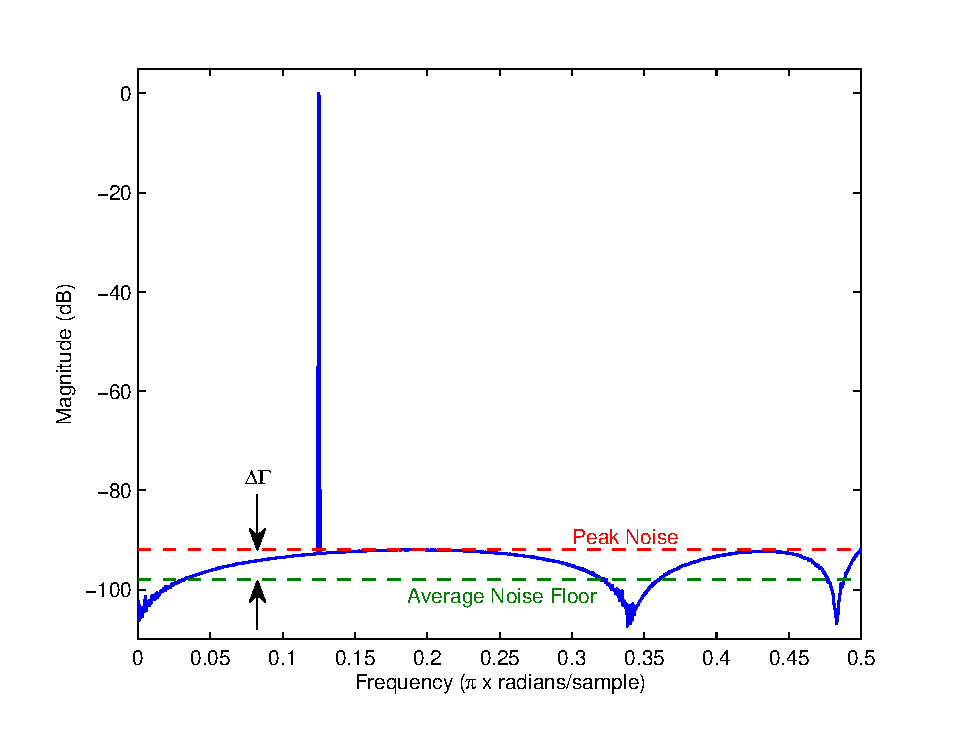
\includegraphics[width=0.8\textwidth]{./matlab_figures/DR_SNR_spectrum}
 \caption{16-bit ADC Output Spectrum}
 \label{fig:DR_SNR_spectrum}
\end{figure}
%-------------------
The difference, $\Delta\Gamma$, between the peak of the noise floor and the average noise
floor results in a loss of effective resolution across much of the spectrum.

%%%%%%%%%%%%%%%%%%%%%%%%%%%%%%%%%%%%%%%%%%%%%%%%
%%% 2.4 Architectures
%%%%%%%%%%%%%%%%%%%%%%%%%%%%%%%%%%%%%%%%%%%%%%%%
\section{Architectures}
Many different types of ADC architectures exist. Selecting the appropriate
architecture for a given application is often a trade-off between size, power
consumption, operational bandwidth, conversion latency, resolution, and sampling rate.
For example, a Nyquist rate converter's resolution is often limited by
its inherent technology. However, system design methods which incorporate signal
processing techniques such as oversampling can increase the effective resolution
of a Nyquist rate converter by reducing its operational bandwidth. Pipelined ADCs use
subranging techniques to parse the sample conversion over several iterations thereby
improving conversion accuracy. Typically, such architectures offer high resolutions over
reasonable operational bandwidths often without the need for additional
post-processing. However, the iterative conversion process requires additional time
thereby increasing conversion latency. For moderate bandwidth applications, specialized
architectures such as $\Delta\Sigma$ modulators are available. Such architectures use
feedback and oversampling to achieve high resolution from relatively simple, low  power 
hardware. 

%%%%%%%%%%%%%%%%%%%%%%%%%%%%%%%%%%%%%%%%%%%%%%%%
%%% 2.4.1 Nyquist Rate converters
%%%%%%%%%%%%%%%%%%%%%%%%%%%%%%%%%%%%%%%%%%%%%%%%
\subsection{Nyquist Rate Converters}
Recall that Nyquist rate converters are ADCs which sample the input at or near its
Nyquist rate, $2f_0$, as defined in \eqref{eq:nyquist}. As such, the sampling frequency,
$f_s$, must be must be at least twice the input signal's Nyquist bandwidth, $f_0$. To
minimize out of band signal energy from aliasing into the operational bandwidth of the
Nyquist rate converter, the input signal is typically bandlimited to $f_s/2$ by an an
anti-aliasing filter prior to being sampled. However, due to practical limitations of this
anti-aliasing filter, Nyquist converters often sample the input signal at a frequency that
is slightly higher than the Nyquist rate.

Nyquist converter bandwidths are typically limited by the electrical properties of
the fabrication process in which they are implemented. With current fabrication processes
capable of supporting signal bandwidths in the GHz range, Nyquist converters are capable
of processing bandlimited signals with bandwidths well in excess of 500 MHz
\cite{ltc2209_datasheet}.
As a result, Nyquist converters offer the widest range of usable bandwidth when compared
to other ADC architectures. However, the effective resolution of Nyquist converters is
typically limited by achievable device density and electronic component matching. As
device geometries decrease, the inherent mismatch of components increases which limits the
converter's achievable resolution.

To illustrate, consider the $B$-bit Flash ADC in Figure \ref{fig:flash_adc}. Such
implementations require $2^B-1$ comparators and $2^B$ resistors. Because the total area
required in an IC to implement a design is proportional to the overall device count and
because the device count of a $B$-bit Flash ADC increases exponentially with $B$, Flash
ADCs with practical dimensions are limited to a resolution of 8-bits for current process
technologies\cite{johns_analog_1996}. Also, Flash ADCs require components to be matched
perfectly to maintain uniform quantization step sizes, $\Delta$. Because nominal
components do not match well over large device geometries, the effective resolution of
Flash based ADCs are typically less than the ideal.
%-------------------
\begin{figure}[htbp]
 \centering
 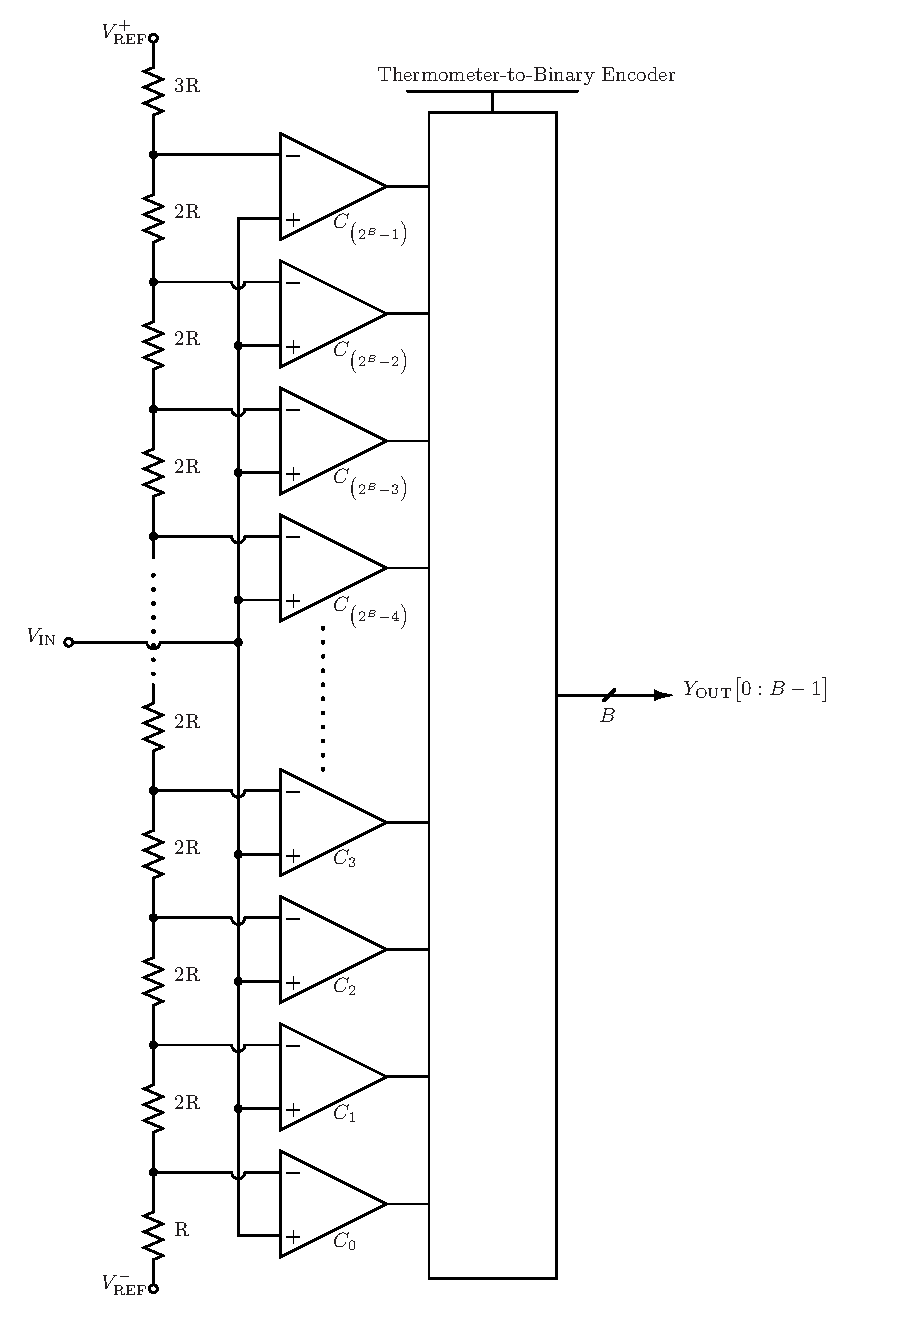
\includegraphics[width=0.9\textwidth]{./final_figures/Flash_ADC.eps}
 \caption{Flash ADC System Block Diagram}
 \label{fig:flash_adc}
\end{figure}
%-------------------

%%%%%%%%%%%%%%%%%%%%%%%%%%%%%%%%%%%%%%%%%%%%%%%%
%%% 2.4.1 Oversampling converters
%%%%%%%%%%%%%%%%%%%%%%%%%%%%%%%%%%%%%%%%%%%%%%%%
\subsection{Oversampling Converters}
Oversampling ADCs are ADCs which increase their effective resolution by
sampling their input signals at much higher rates than its Nyquist rate and
then band-limiting the quantization noise to the Nyquist bandwidth of the input signal.
The ratio of the sampling frequency, $f_s$, to the input signal's Nyquist rate, $2f_0$, is
referred to as the oversampling-rate (OSR) and in this thesis is denoted as $M$; that is, 
%---------------
\begin{equation}\label{eq:OSR}
 M=\frac{f_{s}}{2f_{0}}\text{.}
\end{equation}
%---------------

To illustrate, consider a Nyquist ADC with a sampling frequency, $f_s$, and an input
signal with a Nyquist bandwidth, $f_0$. As illustrated in Figure
\ref{fig:ADC_spectrum_comparison}(a), if $f_s=2f_0$, then the quantization noise is
uniformly distributed over the operational bandwidth, $f_\text{NY}$, where
$f_\text{NY}\in\left[-f_0,f_0\right]$. Alternatively, consider an oversampling ADC with a
sampling frequency, $f_s$, such that $f_s=M2f_0$ where $M$ is the OSR. For such an ADC,
the quantization noise is uniformly distributed over the operational bandwidth,
$f_{\text{OS}}$, where $f_\text{OS}\in \left[-f_s/2, f_s/2\right]$. As illustrated in
Figure \ref{fig:ADC_spectrum_comparison}(b), if the ADC's output is filtered so that it is
bandlimited to the input signal's Nyquist bandwidth, $f_0$, then the quantization noise
power distributed over the remaining frequencies, $f_0\leq\lvert f\rvert\leq Mf_0$, is
effectively removed from the output. Thus, the average quantization noise power is
decreased by a factor of $M$ and the SNR is increased by a factor of $M$ thereby
increasing the ADC's effective resolution. From observation of Figure
\ref{fig:ADC_spectrum_comparison}, the in-band quantization noise for the oversampling
converter is significantly less than the Nyquist converter.

To further illustrate, consider a $B$-bit oversampling ADC that has an OSR, $M$, with a
quantization noise power, $P_e$, that is uniformly distributed over its operational
bandwidth $\left[-f_s/2,f_s/2\right]$, where $f_s$ denotes the sampling frequency. If the
ADC's output is filtered so that the quantization noise power is bandlimited to the input
signal's Nyquist bandwidth, $\left[-f_0,f_0\right]$, the filtered output quantization
noise power, $P_{e,\text{OS}}$, can be expressed as
%---------------
\begin{equation}\label{eq:average_noise_power_only_OSR}
 P_{e,\text{OS}}=\frac{1}{f_s}\int_{-f_0}^{f_0}P_e
d f=P_e\frac{2f_0}{f_s}=\frac{P_e}{M}\text{.}
\end{equation}
%---------------
Thus, the average quantization noise power, $P_{e,\text{OS}}$, for an oversampling ADC
with an OSR, $M$, can be calculated by substituting \eqref{eq:quantization_noise_power}
into \eqref{eq:average_noise_power_only_OSR} which results in
%---------------
\begin{equation}\label{eq:average_noise_power_only_OSR_2}
 P_{e,\text{OS}}=\frac{\Delta^2}{12}\left(\frac{1}{M}\right)
\end{equation}
%---------------
where $\Delta$ corresponds to the quantization step size. Substituting
\eqref{eq:average_noise_power_only_OSR_2} into \eqref{eq:SNR} and solving for the
theoretical SNR for an oversampled Nyquist rate converter which is stimulated by a
full-scale sinusoid as defined by \eqref{eq:fs_sinusoid_power} yields
%---------------
\begin{equation}\label{eq:SNR_OSR}
\begin{split}
\text{SNR}_\text{dB,OS}& =
10\log\frac{\left(\displaystyle\frac{\Delta^22^{2B}}{8}\right)}{\left(\displaystyle\frac
{\Delta^2}{12M}\right)}\\
& =10\log\Bigl(2^{2B}\bigl(3/2\bigr)M\Bigr)\\
& = 6.02B + 1.76+10\log(M)
\end{split}
\end{equation}
%---------------
where $B$ is the number of quantization bits and $M$ is the OSR. Because the maximum OSR
is a function of the ADC's maximum sampling frequency, $M$ is typically selected between 8
and 256. As such, oversampling converters can typically achieve a 9 to 24 dB increase in
SNR which is equivalent to an increase of 1 to 3 bits in effective resolution.

%%%%%%%%%%%%%%%%%%%%%%%%%%%%%%%%%%%%%%%%%%%%%%%%
%%% 2.4.1 Delta Sigma Modulators
%%%%%%%%%%%%%%%%%%%%%%%%%%%%%%%%%%%%%%%%%%%%%%%%
\subsection[Delta Sigma Modulators]{$\Delta\Sigma$ Modulators}
$\Delta\Sigma$ modulators are an ADC architecture that uses oversampling and a feedback
loop to achieve high signal to noise ratios (SNRs) and large dynamic ranges (DRs). Because
of the simplicity of the architecture, $\Delta\Sigma$ modulators can be implemented
using relatively simple analog circuitry in standard CMOS processes which offer low-power
performance and high levels of integration for mixed-signal
electronics\cite{kester_analog_2006}.

To achieve a large DR and high SNR, $\Delta\Sigma$ modulators are designed so that the
quantization noise's feedback loop filter, or noise transfer function (NTF), attenuates
the quantization noise within the frequency band of interest. Additionally, as with other
oversampling ADCs, the $\Delta\Sigma$ modulator's output is bandlimited to the input
signal's Nyquist bandwidth, $f_0$. A comparison of the output spectra for a Nyquist rate
converter, an oversampling converter, and a $\Delta\Sigma$ modulator is shown in Figure
\ref{fig:ADC_spectrum_comparison} (adapted from \cite{kester_ADC_arch_2005}) which
illustrates the relative amount of in-band noise power for each architecture.
As illustrated in Figure \ref{fig:ADC_spectrum_comparison}(c), the amount of
in-band noise power for $\Delta\Sigma$ modulators is largely determined by the shape of
the NTF.
%-------------------
\begin{figure}[H]
 \centering
 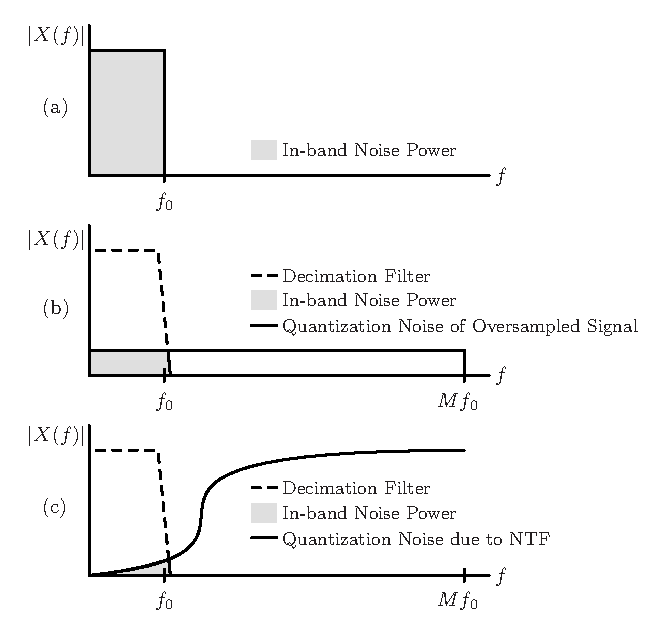
\includegraphics[width=0.8\textwidth]{./final_figures/ADC_spectrum_comparison}
\captionsetup{justification=centering} 
\caption[]{
ADC Output Noise Spectrum Comparison\\
(a) Nyquist Rate Converter 
(b) Oversampling Converter 
(c) $\Delta\Sigma$ Modulator
}
 \label{fig:ADC_spectrum_comparison}
\end{figure}
%-------------------

%%%%%%%%%%%%%%%%%%%%%%%%%%%%%%%%%%%%%%%%%%%%%%%%
%%% 2.4.1 Noise Shaping
%%%%%%%%%%%%%%%%%%%%%%%%%%%%%%%%%%%%%%%%%%%%%%%%
\subsubsection{Noise Shaping}
Figure \ref{fig:linear_block_diagram} illustrates a generic system structure of a
discrete-time $\Delta\Sigma$ modulator. The input block, $F(z)$, is a discrete system that
samples the analog input signal, $x_a(t)$, and processes the resulting discrete-time,
continuous amplitude signal, $x_a(n T_s)$. The ADC
block quantizes, or digitizes, $x_a(n T_s)$ to one of $2^B$ quantization levels, 
where $B$ denotes the number of bits in the digital output, $x(n)$. The
feedback DAC then converts the digital output signal, $x(n)$, into a discrete signal that
is fedback through $H(z)$ and into $G(z)$.
%-------------------
\begin{figure}[htbp]
	\centering
	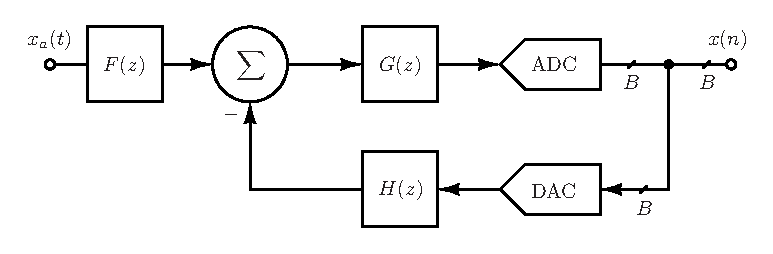
\includegraphics{./final_figures/linear_block_diagram.eps}
	\caption{$\Delta\Sigma$ Modulator Block Diagram}
	\label{fig:linear_block_diagram}
\end{figure}
%-------------------

Figure \ref{fig:linear_simulation_model} illustrates Figure
\ref{fig:linear_block_diagram}'s generic \DS modulator where the ADC's quantizer is
modeled as an additive white noise source. For this thesis, only single-bit quantizers are
considered. As such, the time required for data conversion, or latency through the ADC and
the DAC, can be modeled as a unit delay in the feedback path.
 %-----------------------
\begin{figure}[htbp]
	\centering
	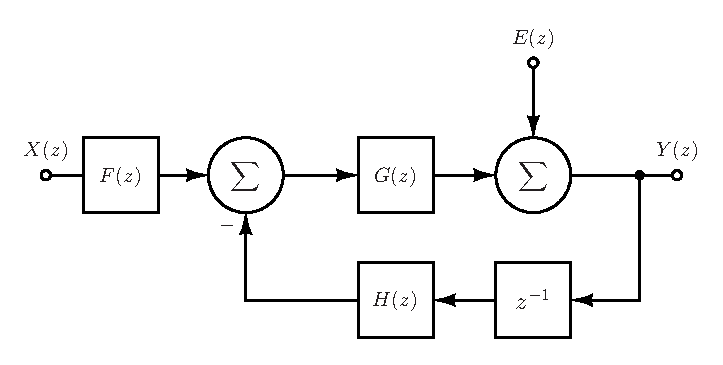
\includegraphics{./final_figures/linear_block_simulation.eps}
	\caption{$\Delta\Sigma$ Modulator Linear Model Block Diagram}
	\label{fig:linear_simulation_model}
\end{figure}
%-----------------------

Because the blocks, $F(z)$, $G(z)$, and $H(z)$ are typically implemented as linear time
invariant (LTI) subsystems, the NTF and STF can be expressed as 
%-----------------------
\begin{equation}\label{eq:STF}
\text{STF}(z)=\frac{Y(z)}{X(z)}=\frac{F(z)G(z)}{1+z^{-1}G(z)H(z)}
\end{equation}
%-----------------------
and
%-----------------------
\begin{equation}\label{eq:NTF}
\text{NTF}(z)=\frac{Y(z)}{E(z)}=\frac{1}{1+z^{-1}G(z)H(z)}\text{.}
\end{equation}
%-----------------------

Figure \ref{fig:DSM_loop_filters} illustrates a STF and NTF for a lowpass $\Delta\Sigma$
modulator where the quantization noise is attenuated by a highpass NTF and the input
signal is filtered by a lowpass STF.
%-----------------------
\begin{figure}[htbp]
	\centering
	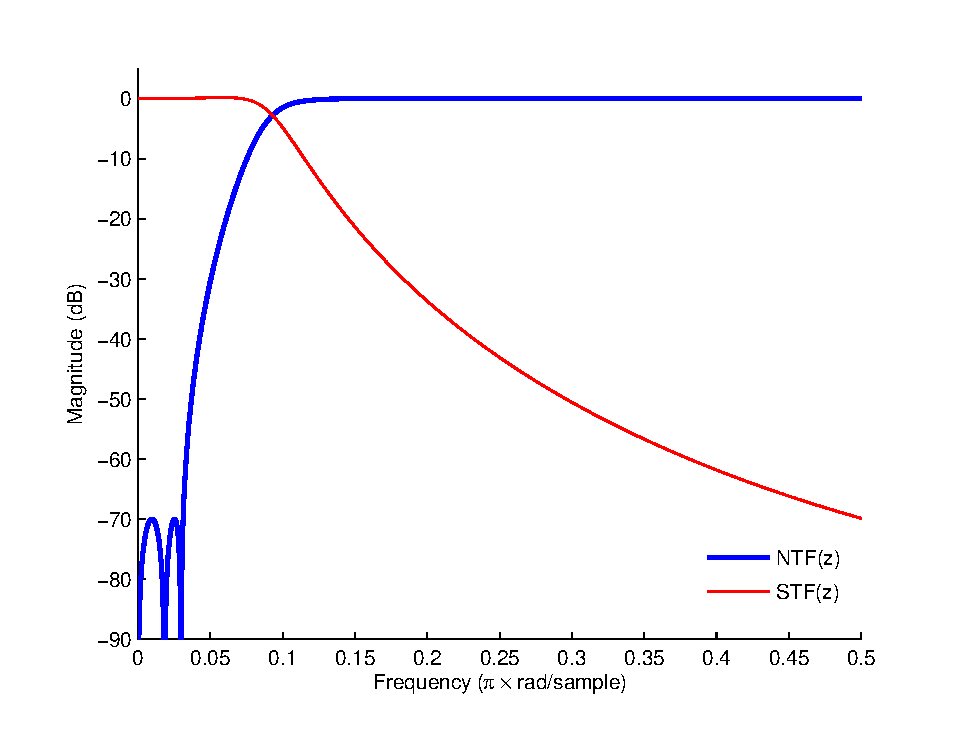
\includegraphics[width=0.65\textwidth]{./matlab_figures/LPDSM_spec_ex}
	\caption[Example: \DS Modulator Magnitude Response]{Examples of a STF and NTF
Magnitude Responses for a Lowpass Discrete-Time \DS Modulator}
	\label{fig:DSM_loop_filters}
\end{figure}
%-----------------------
If the NTF and STF are modeled as LTI systems, the output, $Y(z)$, of a \DS modulator can
be expressed as
%-----------------------
\begin{equation}\label{eq:DSM_output}
 Y(z)=\text{STF}(z)X(z)+\text{NTF}(z)E(z)
\end{equation}
%-----------------------
where $X(z)$ and $E(z)$ correspond to the $\mathcal{z}$-transforms of the input signal
and quantization noise respectively.

\subsection[Delta Sigma Modulator Implementations: Linear Models]
{$\Delta\Sigma$ Modulator Implementations: Linear Models}
The $\Delta\Sigma$ modulator that has been mathematically modeled by the block
diagram shown in Figure \ref{fig:linear_block_diagram} can be implemented using many
different structures. Common hardware implementations include
cascade-of-resonators-feedback (CRFB), cascade-of-resonators-feedforward (CRFF),
cascade-of-integrators-feedback (CIFB), and cascade-of-integrators-feedforward
\cite{schreier_understanding_2004}. For this thesis, a CRFB implementation was
implemented.

\subsubsection{First Order System}
\DS modulator implementations which utilize analog hardware (e.g. integrators) to realize
their loop filters are referred to as continuous-time $\Delta\Sigma$ modulators. For
example, Figure \ref{fig:ct_first_order} illustrates a 1st order, continuous-time \DS
modulator.
%-------------------
\begin{figure}[htbp]
 \centering
 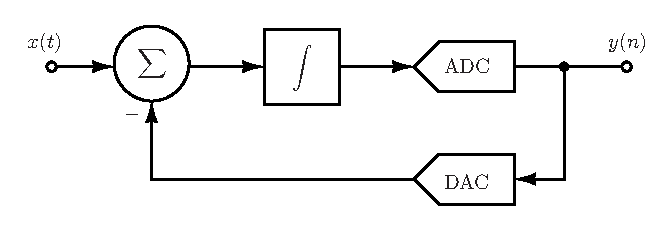
\includegraphics{./final_figures/ct_dsm_model.eps}
 \caption{First-Order \CTDSM}
 \label{fig:ct_first_order}
\end{figure}
%-------------------
Similarly, implementations which utilize discrete-time hardware (e.g. accumulators) to
realize their loop filters  are referred to as discrete-time $\Delta\Sigma$ modulators. As
illustrated in Figures \ref{fig:ct_first_order} and \ref{fig:dt_first_order},
discrete-time \DS modulators typically use an accumulator in place of the
integrators.
%-------------------
\begin{figure}[htbp]
 \centering
 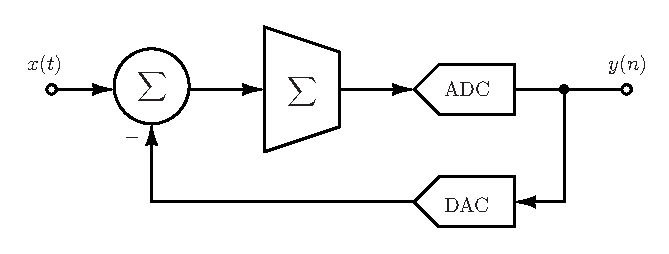
\includegraphics{./final_figures/dt_dsm_model.eps}
 \caption{First-Order \DTDSM}
 \label{fig:dt_first_order}
\end{figure}
%-------------------
Because discrete-time \DS modulators use discrete-time hardware to realize their loop
filters, traditional discrete-time design and analysis techniques can be used
\cite{hayes_schaums_1998}\cite{cherry_continuous-time_1999}.

Figure  \ref{fig:linear_z_model_1} shows a 1st order, discrete-time \DS modulator where 
the quantization noise is modeled as an additive white noise source. 
%-------------------
\begin{figure}[htbp]
 \centering
 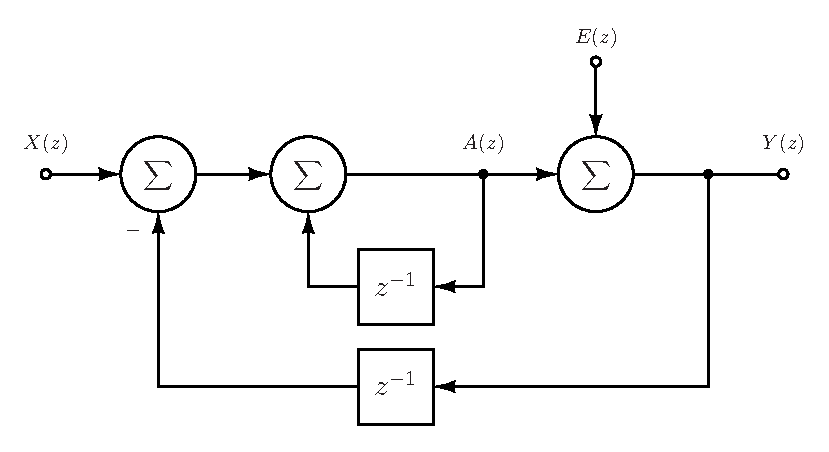
\includegraphics{./final_figures/first_order_simple.eps}
 \caption{First Order Linear Model}
 \label{fig:linear_z_model_1}
\end{figure}
%-------------------
Recall that a $\Delta\Sigma$ modulator's output can be modeled as the sum of the
quantization error and the input signal. For lowpass architectures, the quantization error
is highpass filtered by the NTF and the input signal is lowpass filtered by the STF as
described by \eqref{eq:DSM_output}. From observation of Figure \ref{fig:linear_z_model_1},
the \DS modulator's output, $Y(z)$, is given as
%-------------------
\begin{equation}\label{eq:1st_lin_easy1}
 Y(z)=E(z)+A(z)
\end{equation}
%-------------------
where $A(z)$ is the accumulator output which is given as 
%-------------------
\begin{equation}\label{eq:1st_lin_easy2}
 A(z)=z^{-1}A(z)+X(z)-z^{-1}Y(z)\text{.}
\end{equation}
%-------------------
Substituting \eqref{eq:1st_lin_easy2} into \eqref{eq:1st_lin_easy1}, the output,
$Y(z)$, can be expressed as 
%-------------------
\begin{equation}\label{eq:1st_lin_easy3}
 \begin{split}
  Y(z) &= E(z)+z^{-1}A(z)+X(z)-z^{-1}Y(z)\\
       &= X(z)+E(z)-z^{-1}\bigl(Y(z)-A(z)\bigr)\\
       &= X(z)+\bigl(1-z^{-1}\bigr)E(z)\text{.}
 \end{split}
\end{equation}
%-------------------
Comparing \eqref{eq:1st_lin_easy3} and \eqref{eq:DSM_output}, it can be seen that
%-------------------
\begin{equation}\label{eq:first_order_STF}
   \text{STF}(z)=1
\end{equation}
%-------------------
and
%-------------------
\begin{equation}\label{eq:first_order_NTF}
   \text{NTF}(z)=\left(1-z^{-1}\right)
\end{equation}
%-------------------
which implies that the input signal, $X(z)$, is unaltered at the output and the
quantization noise, $E(z)$, is lowpass filtered by the first order expression
$\left(1-z^{-1}\right)$.

The location of the poles and zeros of the NTF and STF determine the
characteristics of the NTF's and STF's frequency response. However, the \DS modulator
shown in Figure \ref{fig:linear_z_model_1} does not allow the pole and zero locations to
be adjusted. The pole locations can be adjusted by adding feedback
coefficients to the \DS modulator as illustrated in Figure \ref{fig:linear_z_model_2}.
%-------------------
\begin{figure}[htbp]
 \centering
 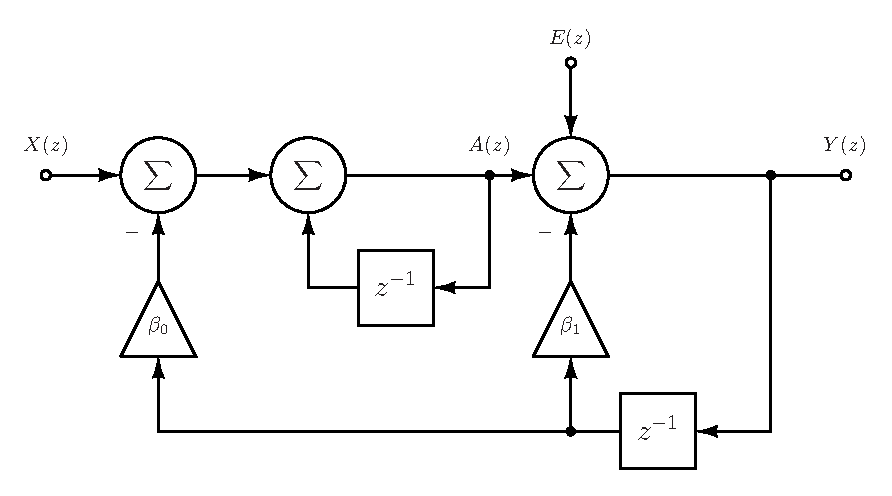
\includegraphics{./final_figures/first_order_linear_model.eps}
 \caption{Generalized First Order Linear Model}
 \label{fig:linear_z_model_2}
\end{figure}
%-------------------
From observation of Figure \ref{fig:linear_z_model_2}, the \DS
modulator's output, $Y(z)$, is given as
%-------------------
\begin{equation}\label{eq:1st_lin_1}
 Y(z)=E(z)+A(z)-\beta_{1}z^{-1}Y(z)
\end{equation}
%-------------------
where $A(z)$ is the accumulator output which is given as 
%-------------------
\begin{equation}\label{eq:1st_lin_2}
 \begin{split}
 A(z)& = z^{-1}A(z)+X(z)-\beta_{0}z^{-1}Y(z)\\
      &   = \frac{X(z)-\beta_{0}z^{-1}Y(z)}{\left(1-z^{-1}\right)}\text{.}
 \end{split}
\end{equation}
%-------------------
Substituting \eqref{eq:1st_lin_2} into \eqref{eq:1st_lin_1} the output,
$Y(z)$, can be expressed as 
%-------------------
\begin{equation}\label{eq:1st_lin_3}
  \begin{split}
  Y(z)& =
E(z)+\frac{X(z)-\beta_{0}z^{-1}Y(z)}{\left(1-z^{-1}\right)}-\beta_{1}z^{-1}Y(z)\\
        & =
\frac{\bigl(1-z^{-1}\bigr)E(z)+X(z)}{\Bigl(1+\bigl(\beta_{0}+\beta_{1}-1\bigr)z^{-1}
-\beta_{1}z^{-2}\Bigr)}\\
     & = \frac{X(z)}{\Bigl(1+\bigl(\beta_{0}+\beta_{1}-1\bigr)z^
{-1}-\beta_{1}z^{-2}\Bigr)}+\frac{\bigl(1-z^{-1}\bigr)E(z)}{\Bigl(1+\bigl(\beta_{0}
 +\beta_{1}-1\bigr)z^{-1}-\beta_{1}z^{-2}\Bigr)}\text{.}
 \end{split}
\end{equation}
%-------------------
Comparing \eqref{eq:1st_lin_3} and \eqref{eq:DSM_output}, it can be seen that
%-------------------
\begin{equation}\label{eq:1st_lin_STF}
   \text{STF}(z)=
\frac{1}{\Bigl(1+\bigl(\beta_{0}+\beta_{1}-1\bigr)z^{-1}-\beta_{1}z^{-2}\Bigr)}
\end{equation}
%-------------------
and
%-------------------
\begin{equation}\label{eq:1st_lin_NTF}
 \text{NTF}(z)=
	\frac{\bigl(1-z^{-1}\bigr)}{\Bigl(1+\bigl(\beta_{0}+\beta_{1}-1\bigr)z^{-1}-
	\beta_{1}z^{-2}\Bigr)}\text{.}
\end{equation}
%-------------------
For most applications, $\beta_1=0$. For such applications the transfer
functions described by \eqref{eq:1st_lin_STF} and \eqref{eq:1st_lin_NTF} can be
written as
%-------------------
\begin{equation}\label{eq:1st_lin_STF_reduced}
   \text{STF}(z)=
\frac{1}{1+\left(\beta_{0}-1\right)z^{-1}}
\end{equation}
%-------------------
and
%-------------------
\begin{equation}\label{eq:1st_lin_NTF_reduced}
 \text{NTF}(z)=
	\frac{\left(1-z^{-1}\right)}{1+\left(\beta_{0}-1\right)z^{-1}}
\end{equation}
%-------------------
respectively. Thus, \eqref{eq:1st_lin_STF_reduced} and \eqref{eq:1st_lin_NTF_reduced} are
equivalent to \eqref{eq:first_order_STF} and \eqref{eq:first_order_NTF} when $\beta_0=1$.

%%%%%%%%%%%%%%%%%%%%%%%%%%%%%%%%%%%%%%%%%%%%%%%%%%%%%%%%%%%%%%%%%%%%%%%%%%%%%%%%
\subsubsection{Second Order System}
Because the NTFs of 1st order $\Delta\Sigma$ modulators have a limited amount of
quantization noise attenuation, higher order systems are generally used. Consider the
second order system illustrated in Figure \ref{fig:linear_z_model_2nd_order}. This
system can be formed by cascading two first order systems together. 
%-------------------
\begin{figure}
  \centering
  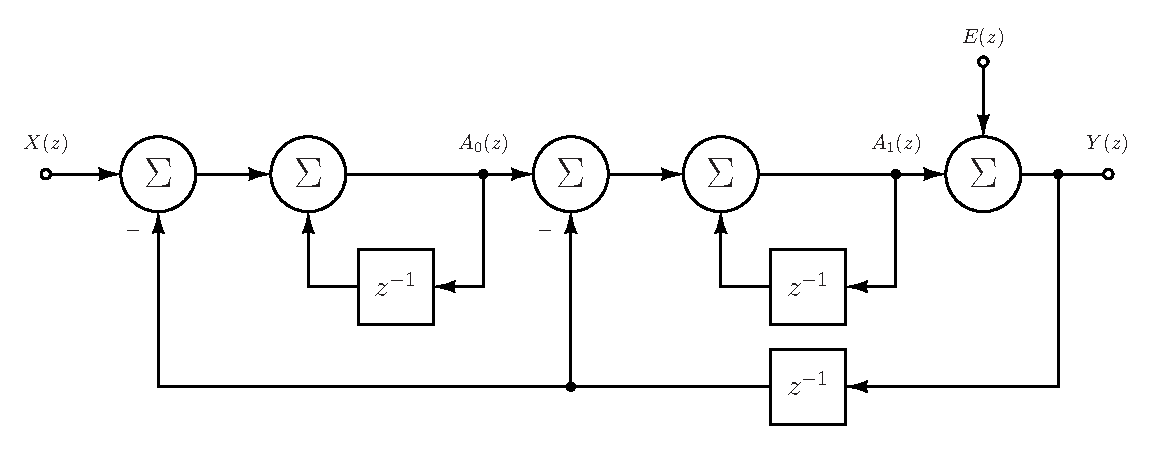
\includegraphics[width=\textwidth]{./final_figures/second_order_simple_model.eps}
  \caption{Second Order Linear Model}
  \label{fig:linear_z_model_2nd_order}
\end{figure}
%-------------------
From observation of Figure \ref{fig:linear_z_model_2nd_order}, the second order \DS
modulator's output, $Y(z)$, is given
as
%-------------------
\begin{equation}\label{eq:2nd_order_DSM_output_1}
 Y(z)=E(z)+A_1(z)
\end{equation}
%-------------------
where $A_1(z)$ corresponds to the output of the second accumulator. The accumulator
outputs, $A_{0}$ and $A_{1}$, can be expressed as
%-------------------
\begin{equation}\label{eq:2nd_order_DSM_accumulator_0}
  A_{0}(z) = \frac{X(z)-z^{-1}Y(z)}{1-z^{-1}}
 \end{equation}
 %-------------------
and
%-------------------
\begin{equation}\label{eq:2nd_order_DSM_accumulator_1}
  A_{1}(z) = \frac{A_{0}(z)-z^{-1}Y(z)}{1-z^{-1}}\text{.}
\end{equation}
%-------------------
Substituting \eqref{eq:2nd_order_DSM_accumulator_0} into
\eqref{eq:2nd_order_DSM_accumulator_1} and the result into
\eqref{eq:2nd_order_DSM_output_1}, the
output, $Y(z)$, can be expressed as 
%-------------------
\begin{equation}\label{eq:2nd_order_DSM_output}
  Y(z) = X(z)+ \bigl(1-z^{-1}\bigr)^2 E(z)\text{.}
\end{equation}
%-------------------
Comparing \eqref{eq:2nd_order_DSM_output} and \eqref{eq:DSM_output}, it can be seen that
%-------------------
\begin{equation}\label{eq:second_order_STF}
   \text{STF}(z)=1
\end{equation}
%-------------------
and
%-------------------
\begin{equation}\label{eq:second_order_NTF}
   \text{NTF}(z)=\left(1-z^{-1}\right)^2
\end{equation}
%-------------------
which implies that the input signal, $X(z)$, is unaltered at the output and the
quantization noise, $E(z)$, is lowpass filtered by the second order expression
$\left(1-z^{-1}\right)^2$.

To adjust the pole locations of the 2nd order \DS modulator shown in Figure
\ref{fig:linear_z_model_2nd_order} feedback coefficients, denoted as $\beta_0$, $\beta_1$,
 and $\beta_2$, can be added as shown in Figure
\ref{fig:linear_z_model_2nd_order_complex}. 
%-------------------
\begin{figure}
  \centering
  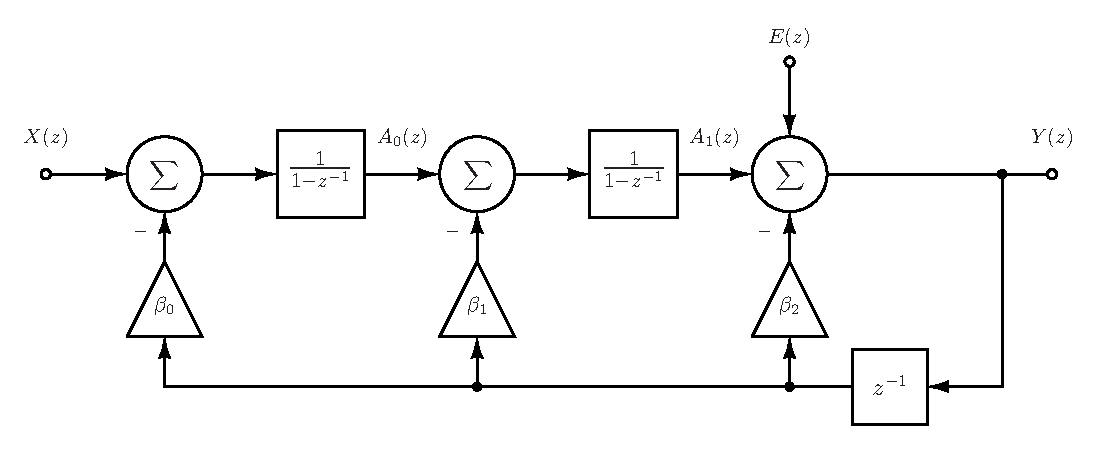
\includegraphics[width=\textwidth]{./final_figures/second_order_complex_model.eps}
  \caption{Generalized Second Order Linear Model}
  \label{fig:linear_z_model_2nd_order_complex}
\end{figure}
%-------------------
From observation of Figure \ref{fig:linear_z_model_2nd_order_complex}, the \DS
modulators's output, $Y(z)$, is given as 
%-------------------
\begin{equation}\label{eq:2nd_order_DSM_output_complex_1}
 Y(z) = E(z)+A_1(z)-\beta_2 z^{-1}Y(z)
\end{equation}
%-------------------
where $A_1(z)$ corresponds to the output of the second accumulator. The accumulator
outputs, $A_{0}$ and $A_{1}$, can be expressed as
%-------------------
\begin{equation}\label{eq:2nd_order_DSM_accumulator_0_complex}
  A_{0}(z) = \frac{X(z)-\beta_0 z^{-1}Y(z)}{1-z^{-1}} 
\end{equation}
%-------------------
and
%-------------------
\begin{equation}\label{eq:2nd_order_DSM_accumulator_1_complex}
  A_{1}(z) = \frac{A_{0}(z)-\beta_1 z^{-1}Y(z)}{1-z^{-1}}=\frac{X(z)-(\beta_0+\beta_1)
z^{-1}Y(z)}{\left(1-z^{-1}\right)^2}
\end{equation}
%-------------------
Substituting \eqref{eq:2nd_order_DSM_accumulator_0_complex} into 
\eqref{eq:2nd_order_DSM_accumulator_1_complex} and the result into 
\eqref{eq:2nd_order_DSM_output_complex_1}, the
output, $Y(z)$, can be expressed as 
%-------------------
\begin{equation}\label{eq:2nd_order_DSM_output_complex}
 \begin{split}
  Y(z)& = E(z)+\frac{X(z)-(\beta_0+\beta_1)
z^{-1}Y(z)}{\left(1-z^{-1}\right)^2}-\beta_2 z^{-1}Y(z) \\
       & = \frac{X(z)+ \bigl(1-z^{-1}\bigr)^2 E(z)}
{ 1+ z^{-1}\bigl(-2+\beta_0+\beta_1+\beta_2\bigr)
   + z^{-2}\bigl(1-\beta_1-2\beta_2\bigr)
   + z^{-3}\beta_2}.\\
 \end{split}
\end{equation}
%-------------------
Comparing \eqref{eq:2nd_order_DSM_output_complex} and \eqref{eq:DSM_output}, it can be
seen that
%-------------------
\begin{equation}\label{eq:second_order_STF_complex}
   \text{STF}(z)= \frac{1}{
  1+ z^{-1}\bigl(-2+\beta_0+\beta_1+\beta_2\bigr)
   + z^{-2}\bigl(1-\beta_1-2\beta_2\bigr)
   + z^{-3}\beta_2}
\end{equation}
%-------------------
and
%-------------------
\begin{equation}\label{eq:second_order_NTF_complex}
   \text{NTF}(z)=\frac{\bigl(1-z^{-1}\bigr)^2 }{
  1+ z^{-1}\bigl(-2+\beta_0+\beta_1+\beta_2\bigr)
   + z^{-2}\bigl(1-\beta_1-2\beta_2\bigr)
   + z^{-3}\beta_2}\text{.}
\end{equation}
%-------------------

For most applications, $\beta_2=0$. For such applications the transfer functions
described by \eqref{eq:second_order_STF_complex} and
\eqref{eq:second_order_NTF_complex}) can be written as
%-------------------
\begin{equation}\label{eq:2nd_lin_STF_reduced}
   \text{STF}(z)= \frac{1}{
  1+ z^{-1}\bigl(-2+\beta_0+\beta_1\bigr)
   + z^{-2}\bigl(1-\beta_1\bigr)}
\end{equation}
%-------------------
and
%-------------------
\begin{equation}\label{eq:2nd_lin_NTF_reduced}
   \text{NTF}(z)=\frac{\left(1-z^{-1}\right)^2 }{
  1+ z^{-1}\bigl(-2+\beta_0+\beta_1\bigr)
   + z^{-2}\bigl(1-\beta_1\bigr)}
\end{equation}
%-------------------
respectively. Thus, \eqref{eq:2nd_lin_STF_reduced} and
\eqref{eq:2nd_lin_NTF_reduced} are
equivalent to \eqref{eq:second_order_STF} and \eqref{eq:second_order_NTF} when
$\beta_0=\beta_1=1$.

Because a \DS modulator's NTF is designed first, the feedback coefficients,
$\{\beta_n\}$, 
are chosen to optimize the NTF's characteristics. As such, the STFs in
\eqref{eq:second_order_STF_complex} and \eqref{eq:2nd_lin_STF_reduced} are fixed by the
NTF's design. To shape the STF, feedforward coefficients can be added to Figure
\ref{fig:linear_z_model_2nd_order_complex} as illustrated in Figure
\ref{fig:general_2nd_order}.
%-------------------
\begin{figure}
  \centering
  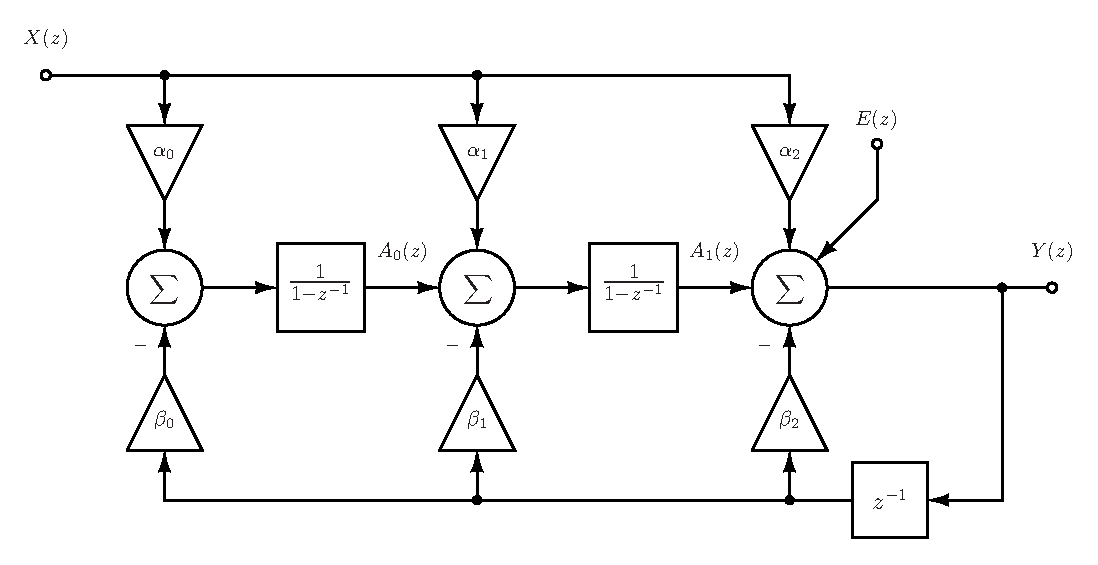
\includegraphics[width=\textwidth]{./final_figures/general_2nd_order.eps}
  \caption[Second Order Linear Model with Feedforward Coefficients]{Generalized Second
Order Linear Model with Feedforward Coefficients}
  \label{fig:general_2nd_order}
\end{figure}
%-------------------
From observation of Figure \ref{fig:general_2nd_order}, the \DS modulator's output,
$Y(z)$, is given as 
%-------------------
\begin{equation}\label{eq:2nd_order_DSM_output_general}
 Y(z)=E(z)+\alpha_2 X(z)+A_1(z)-\beta_2 z^{-1}Y(z)
\end{equation}
%-------------------
where $A_1(z)$ corresponds to the output of the second accumulator. The accumulator
outputs, $A_{0}$ and $A_{1}$, can be expressed as
%-------------------
\begin{equation}\label{eq:2nd_order_DSM_accumulator_0_general}
  A_{0}(z) = \frac{\alpha_0 X(z)-\beta_0 z^{-1}Y(z)}{1-z^{-1}} 
\end{equation}
%-------------------
and
%-------------------
\begin{equation}\label{eq:2nd_order_DSM_accumulator_1_general}
  A_{1}(z) = \frac{\alpha_1 X(z)+ A_{0}(z)-\beta_1 z^{-1}Y(z)}{1-z^{-1}}\text{.}
\end{equation}
%-------------------
Substituting \eqref{eq:2nd_order_DSM_accumulator_0_general} into
\eqref{eq:2nd_order_DSM_accumulator_1_general} and the result into
\eqref{eq:2nd_order_DSM_output_general}, the
output, $Y(z)$, can be expressed as 
%-------------------
\begin{equation}\label{eq:2nd_order_DSM_output_general_2}
\begin{split}
 Y(z)& =\left(\frac{
\bigl(\alpha_0+\alpha_1+\alpha_2\bigr)-z^{-1}\bigl(\alpha_1+2\alpha_2\bigr)+z^{-2}\alpha_2
}
{  1+ z^{-1}\bigl(-2+\beta_0+\beta_1+\beta_2\bigr)
   + z^{-2}\bigl(1-\beta_1-2\beta_2\bigr)
   + z^{-3}\beta_2}\right) X(z)\\
&\quad + \left(\frac{\bigl(1-z^{-1}\bigr)^2}
{  1+ z^{-1}\bigl(-2+\beta_0+\beta_1+\beta_2\bigr)
   + z^{-2}\bigl(1-\beta_1-2\beta_2\bigr)
   + z^{-3}\beta_2}\right)E(z)\text{.}
\end{split}
\end{equation}
%-------------------
Comparing \eqref{eq:2nd_order_DSM_output_general_2} and \eqref{eq:DSM_output}, it can
be seen that
%-------------------
\begin{equation}\label{eq:second_order_STF_general_2_STF}
   \text{STF}(z)= \frac{
\bigl(\alpha_0+\alpha_1+\alpha_2\bigr)-z^{-1}\bigl(\alpha_1+2\alpha_2\bigr)+z^{-2}\alpha_2
}
{  1+ z^{-1}\bigl(-2+\beta_0+\beta_1+\beta_2\bigr)
   + z^{-2}\bigl(1-\beta_1-2\beta_2\bigr)
   + z^{-3}\beta_2}
\end{equation}
%-------------------
and
%-------------------
\begin{equation}\label{eq:second_order_STF_general_2_NTF}
   \text{NTF}(z)=
\frac{\bigl(1-z^{-1}\bigr)^2}
{  1+ z^{-1}\bigl(-2+\beta_0+\beta_1+\beta_2\bigr)
   + z^{-2}\bigl(1-\beta_1-2\beta_2\bigr)
   + z^{-3}\beta_2}\text{.}
\end{equation}
%-------------------
It can be observed from \eqref{eq:second_order_STF_general_2_STF} and
\eqref{eq:second_order_STF_general_2_NTF} that the feedforward coefficients, $\alpha_0$,
$\alpha_1$, and $\alpha_2$, only affect the STF and not the NTF. As such, this allows the
shape of the STF to be
changed independently from the NTF. It also can be seen that
\eqref{eq:second_order_STF_general_2_STF} and \eqref{eq:second_order_STF_general_2_NTF}
are equivalent to
\eqref{eq:second_order_STF_complex} and \eqref{eq:second_order_NTF_complex} for
$\alpha_1=\alpha_2=0$ and $\alpha_0=1$.

\subsubsection{High Order Systems}
Theoretically, a \DS modulator's order, $n$, has no upper bound and thus, the NTF's
stopband attenuation can be increased to any arbitrarily large level. This in turn would
allow the effective resolution of the \DS modulator to increase without bound. However,
physical phenomena such as thermal noise and clock jitter typically limit a \DS
modulator's achievable effective resolution. Therefore, in practice, $\Delta\Sigma$
modulators are typically designed such that $n\leq8$. 

Additionally, because the internal voltage swings of a \DS modulator are limited by the
electrical characteristics of its process technology, scaling coefficients are
typically placed between adjacent integrators to avoid saturation. Saturation, or
clipping, can cause instability and introduces nonlinear distortion thereby decreasing
the effective resolution of the $\Delta\Sigma$ modulator. Figure
\ref{fig:linear_z_model_nth_order} illustrates a generalized $n$th order converter
topology with scaling coefficients, denoted $c_x$, between adjacent integrators where $x$
corresponds to the coefficient's respective integrator number.
%-------------------
\begin{sidewaysfigure}[htbp]
  \centering
  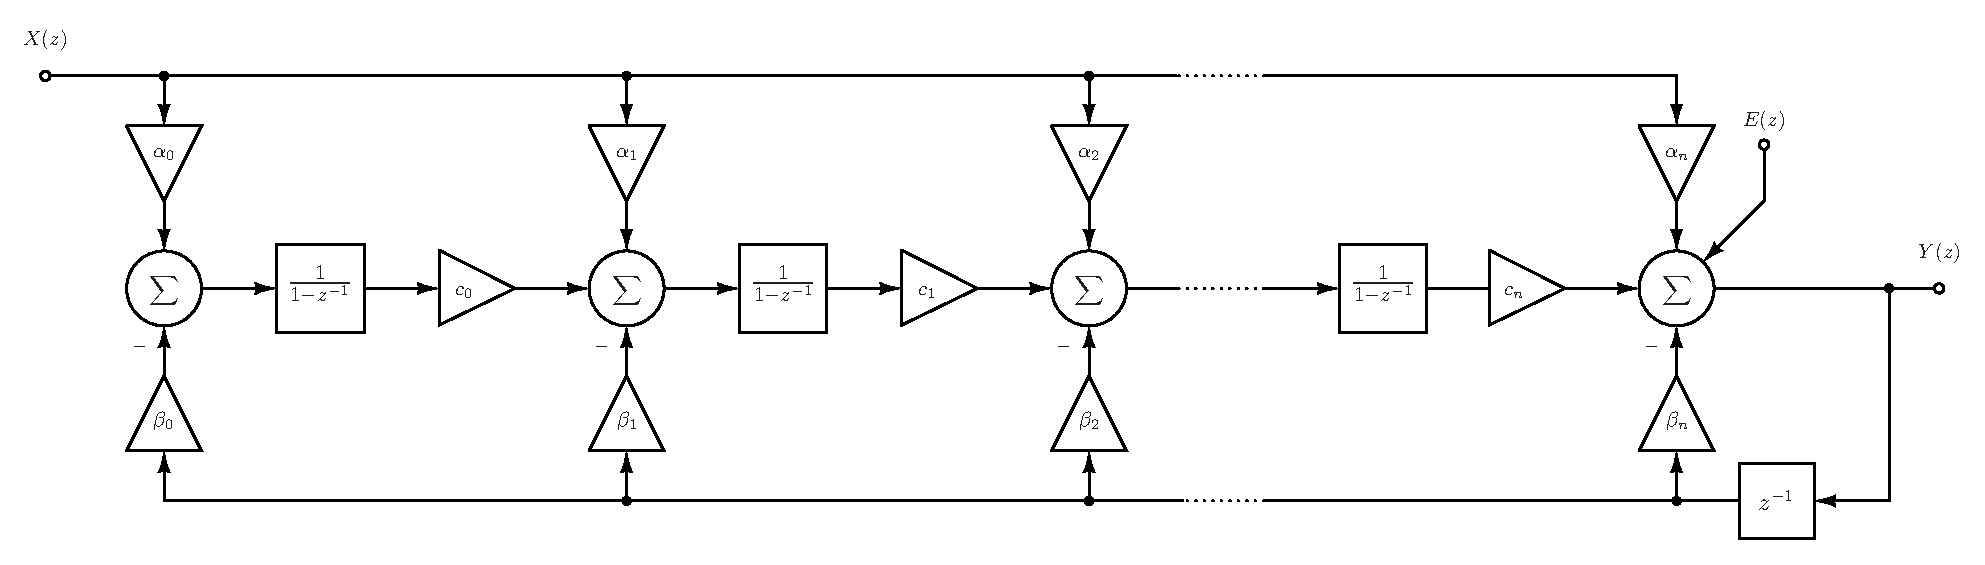
\includegraphics[width=\textwidth]{./final_figures/general_nth_order_2.eps}
  \caption{Generalized $n$th Order Linear Model}
  \label{fig:linear_z_model_nth_order}
\end{sidewaysfigure}
%-------------------

%%%%%%%%%%%%%%%%%%%%%%%%%%%%%%%%%%%%%%%%%%%%%%%%
%%% 2.4.5 DSM Theoretical Performance
%%%%%%%%%%%%%%%%%%%%%%%%%%%%%%%%%%%%%%%%%%%%%%%%
\subsection[Delta Sigma Modulator Theoretical Performance]
{$\Delta\Sigma$ Modulator Theoretical Performance}
The theoretical effective resolution of a \DS modulator can be calculated if the shape of
in-band NTF is known. That is, stochastic system theory can be used to predict the
performance of a deterministic system function for a particular input, $x(n)$, and
the randomly modeled quantization noise, $q(n)$. 

Stochastic system theory states that for an LTI system, an input signal, $x(n)$, which
can be modeled as a discrete-time random process, will produce an output
signal, $y(n)$, which can also be modeled as a discrete-time random
process\cite{papoulis_probability_1984}. As such, descriptive statistics (e.g. mean,
variance, and autocorrelation) are often used to analyze LTI system's output signals when
the input signals can be modeled as random processes.

The autocorrelation, $R_{x(n)}(k)$, of a discrete-time random process, $x(n)$,
can be expressed as
%----------------------
\begin{equation}\label{eq:autocorrelation}
 R_{x(n)}(k)=E\left[x(n)x(n+k)\right]
\end{equation}
%----------------------
where $E[\cdot]$ denotes the expectation operator as defined in
\eqref{eq:discrete_ensemble_average}\cite{hsu_schaums_1996}. If $x(n)$ is a zero mean,
random process then the autocorrelation of $x(n)$ for $k=0$, $R_{x(n)}(0)$, is equivalent
to the variance, $\sigma^2_{x(n)}$, of $x(n)$, as described by
\eqref{eq:expectation_proof}; that is,
%----------------------
\begin{equation}\label{eq:autocorrelation_zero_1}
 R_{x(n)}(0)=E\left[x(n)x(n+0)\right]=E\left[x^2(n)\right]=\sigma^2_{x(n)}\text{.}
\end{equation}
%----------------------
As such, the average power, $P_{x(n)}$, of a zero mean, random process, $x(n)$, can be
expressed as 
%----------------------
\begin{equation}\label{eq:autocorrelation_zero_2}
 P_{x(n)}=R_{x(n)}(0)\text{.}
\end{equation}
%----------------------

It has been shown \cite{oppenheim_discrete-time_1999} that the power spectral
density, $\bm{S}_{x(n)}(e^{j\omega})$, of a discrete-time random process,
$x(n)$, can be calculated by taking the Fourier transform of its autocorrelation,
$R_{x(n)}(k)$; that is,
%----------------------
\begin{equation}\label{eq:power_spectrum}
 \bm{S}_{x(n)}(e^{j\omega})=\sum_{k=-\infty}^{\infty}{R_{x(n)}(k)e^{
-j\omega k}}
\end{equation}
%----------------------
where $\omega$ denotes frequency in radians per sample. Conversely, the autocorrelation of
a discrete-time random process, $R_{x(n)}(k)$, can be calculated by taking the inverse
Fourier transform of its power spectral density, $\bm{S}_{x(n)}(e^{j\omega})$, which
implies that 
%----------------------
\begin{equation}\label{eq:autocorrelation_psd}
 R_{x(n)}(k)=\frac{1}{2\pi}\int_{-\pi}^{\pi}{\bm{S}_{x(n)}(e^{j\omega})
e^{j\omega k} d\omega} \text{.}
\end{equation}
%----------------------
It has also been shown \cite{hsu_schaums_1996}\cite{oppenheim_discrete-time_1999} that
the output power spectral density, $\bm{S}_{y(n)}(e^{j\omega})$, of a LTI
system that has a frequency response, $H(e^{j\omega})$, can be calculated by
taking the product of the input power spectral density,
$\bm{S}_{x(n)}(e^{j\omega})$, and the magnitude-squared of the
system's frequency response; that is, 
%----------------------
\begin{equation}\label{eq:LTI_psd}
 \bm{S}_{y(n)}(e^{j\omega})=\lvert
H(e^{j\omega})\rvert^2\bm{S}_{x(n)}(e^{j\omega})\text{.}
\end{equation}
%----------------------
Therefore using \eqref{eq:autocorrelation_psd} and \eqref{eq:LTI_psd}, the
autocorrelation,
$R_{y(n)}(k)$, of the output, $y(n)$, of an LTI system that has the input $x(n)$ can be
written as
%----------------------
\begin{equation}\label{eq:LTI_output_autocorrelation}
\begin{split}
R_{y(n)}(k)& =\frac{1}{2\pi}\int_{-\pi}^{\pi}\bm{S}_{y(n)}(e^{j\omega})e^{
j\omega k} d\omega\\
& = \frac{1}{2\pi}\int_{-\pi}^{\pi}
\lvert H(e^{j\omega})\rvert^2\bm{S}_{x(n)}(e^{j\omega})e^{
j\omega k} d\omega.
\end{split}
\end{equation}
%----------------------
Using \eqref{eq:autocorrelation_zero_2} and \eqref{eq:LTI_output_autocorrelation}, the
average output power, $P_{y(n)}$, of an LTI system can be calculated as
%----------------------
\begin{equation}\label{eq:LTI_average_output_power}
P_{y(n)}=R_{y(n)}(0)=\frac{1}{2\pi}\int_{-\pi}^{\pi}
\lvert
H(e^{j\omega})\rvert^2\bm{S}_{x(n)}(e^{j\omega})d\omega\text{.}
\end{equation}
%----------------------

Because a \DS modulator's NTF is modeled as a LTI system, its output quantization noise
power, $P_{q(n)}$, can be calculated using \eqref{eq:LTI_average_output_power}; that is,
%---------------
\begin{equation}\label{eq:average_noise_power_NTF}
 P_{q(n)}=\frac{1}{2\pi}\int_{-\omega_0}^{\omega_0}{\lvert
\text{NTF}(e^{j\omega})\rvert^2\bm{S}_{e(n)}(e^{j\omega})d\omega}
\end{equation}
%---------------
where $\omega_0$ corresponds to the Nyquist frequency of the input signal in radians per
sample.

To determine the quantization noise power spectral density, $\bm{S}_{e(n)}(e^{j\omega})$,
the quantization noise is assumed to be a zero mean, uncorrelated white noise process,
which implies that its autocorrelation, $R_{e(n)}(k)$, can be written as
%---------------
\begin{equation}\label{eq:quantization_noise_psd_2}
R_{e(n)}(k)=E\left[e(n)e(n+k)\right]=E\left[e^2(n)\right]\delta(k)=\sigma^2_{e(n)}
\delta(k).
\end{equation}
%---------------
Therefore, the power spectral density of the quantization noise,
$\bm{S}_{e(n)}(e^{j\omega})$, can be written as
%---------------
\begin{equation}\label{eq:quantization_noise_psd_3}
\bm{S}_{e(n)}(e^{j\omega})=\sum_{k=-\infty}^{\infty}\sigma^2_{e(n)}
\delta(k)e^{-j\omega k}=\sigma^2_{e(n)}=P_{e(n)}.
\end{equation}
%---------------
Thus, substituting \eqref{eq:quantization_noise_power} into
\eqref{eq:quantization_noise_psd_3}, it can be seen that 
%---------------
\begin{equation}\label{eq:quantization_noise_psd_6}
\bm{S}_{e(n)}(e^{j\omega})=\frac{\Delta^2}{12}
\end{equation}
%---------------
where $\Delta$ is the quantization interval. Substituting
\eqref{eq:quantization_noise_psd_6} into \eqref{eq:average_noise_power_NTF}, the  \DS
modulator's output quantization noise power, $P_{q(n)}$, can be expressed as
%---------------
\begin{equation}\label{eq:average_noise_power_NTF_2}
\begin{split}
P_{q(n)}& = \frac{1}{2\pi}\int_{-\omega_0}^{\omega_0}{
\lvert
\NTF(e^{j\omega})\rvert^2\bm{S}_{e(n)}(e^{j\omega})d\omega}\\
&
=\frac{1}{2\pi}\left(\frac{\Delta^2}{12}\right)\int_{-\omega_0}^{\omega_0}{
\lvert\NTF(e^{j\omega})\rvert^2d\omega}
\end{split}
\end{equation}
%---------------
where $\omega_0$ corresponds to the input signal's Nyquist bandwidth.

For the $n$th order discrete-time \DS modulator architecture shown in Figure
\ref{fig:linear_z_model_nth_order} where $a_n=b_n=c_n=1$, the NTF can be written as 
%---------------
\begin{equation}\label{eq:NTF_simple_z}
\NTF(z)=(1-z^{-1})^n
\end{equation}
%---------------
which implies that 
%---------------
\begin{equation}\label{eq:NTF_simple_jw}
\NTF(e^{j\omega})=(1-e^{-j\omega})^n=\Biggl(j2e^{-j\frac{\omega}{2}}
\left(\frac{e^{j\frac{\omega}{2}}-e^{-j\frac{\omega}{2}}}{j2}\right)\Biggr)^n.
\end{equation}
%---------------
Using Euler's identity\cite{thomas_thomas_2004}, \eqref{eq:NTF_simple_jw} can be written
as
%---------------
\begin{equation}\label{eq:NTF_simple_euler}
\NTF(e^{j\omega})=\biggl(j2e^{-j\frac{\omega}{2}}\sin\left(\frac{\omega}{2}
\right)\biggr)^n.
\end{equation}
%---------------
Thus, 
%---------------
\begin{equation}\label{eq:NTF_simple_magnitude}
\lvert \NTF(e^{j\omega})\rvert^2=\biggl\lvert
\biggl(j2e^{-j\frac{\omega}{2}}\sin\left(\frac{\omega}{2}
\right)\biggr)^n \biggr\rvert^2 = \biggl(2\sin\left(\frac{\omega}{2}\right)\biggr)^{2n}.
\end{equation}
%---------------
Substituting \eqref{eq:NTF_simple_magnitude} into \eqref{eq:average_noise_power_NTF_2},
the quantization noise power, $P_{q(n)}$, can be written as
%---------------
\begin{equation}\label{eq:quantization_power_some_more_fun}
P_{q(n)}=\frac{1}{2\pi}\left(\frac{\Delta^2}{12}\right)
\int_{-\omega_0}^{\omega_0}\biggl(2\sin\left(\frac{\omega}{2}\right)\biggr)^{2n}
d\omega.
\end{equation}
%---------------
For large OSRs, $\omega_0\ll\pi$, and therefore,
$$\sin\left(\frac{\omega}{2}\right)\approx\frac{\omega}{2}.$$
\cite{schreier_understanding_2004}\cite{thomas_thomas_2004}\cite{kozak_oversampled_2003}.
Substituting this approximation into \eqref{eq:quantization_power_some_more_fun}, the
output quantization noise power, $P_{q(n)}$, can be given as 
%---------------
\begin{equation}\label{eq:average_noise_power_NTF_3}
\begin{split}
P_{q(n)}&
=\frac{1}{2\pi}\left(\frac{\Delta^2}{12}\right)\int_{-\omega_0}^{\omega_0}\omega^{2n}
d\omega\\
& =
\frac{1}{2\pi}\left(\frac{\Delta^2}{12}\right)\left(\frac{\omega^{2n+1}}{2n+1}\biggl\vert_
{-\omega_0 }^{ \omega_0}\right)\\
&
=\frac{\Delta^2}{12\pi}\left(\frac{1}{2n+1}\right)\omega_0^{2n+1}.
\end{split}
\end{equation}
%---------------
Substituting $\omega_0=\pi/M$ into \eqref{eq:average_noise_power_NTF_3}, the
output quantization noise power, $P_{q(n)}$, can be expressed as
%---------------
\begin{equation}\label{eq:average_noise_power_NTF_4}
P_{q(n)}=\frac{\Delta^2}{12\pi}\left(\frac{1}{2n+1}\right)
\left(\frac{\pi}{M}\right)^{2n+1}
\end{equation}
%---------------
where $M$ denotes the OSR.

The theoretical $\text{SNR}_{\text{dB}}$, $\text{SNR}_\text{dB,LPDSM}$, for a lowpass
$\Delta\Sigma$ modulator that has a full-scale sinusoidal input as defined by
\eqref{eq:fs_sinusoid_power}, can be derived by substituting
\eqref{eq:average_noise_power_NTF_4} into \eqref{eq:SNR} such that
%---------------
\begin{equation}\label{eq:SNR_DSM}
\begin{split}
\text{SNR}_\text{dB,LPDSM}& =
10\log\frac{\left(\displaystyle\frac{\Delta^22^{2B}}{8}\right)}
{\displaystyle\frac{\Delta^2}{12\pi}\left(\frac{1}{2n+1}\right)
    \left(\frac{\pi}{M}\right)^{2n+1}}\\
&
=10\log\left(\frac{3}{2}2^{2B}
\right)+10\log\left(2n+1\right)-2n10\log(\pi)+(2n+1)10\log (M)
\\
& = 6.02B + 10\log(2n+1) - 20n\log(\pi)+(20n+10)\log(M)
\end{split}
\end{equation}
%---------------
where $M$ corresponds to the OSR and $B$ corresponds to the number of quantization
bits.
 
From observation of \eqref{eq:SNR_DSM}, it can be seen that the dominant term, that is the
term which has the greatest impact on SNR, in \eqref{eq:SNR_DSM} is $(20n+10)\log(M)$ for
$M\gg1$ which implies that the effective resolution for a $\Delta\Sigma$ modulator is
largely determined by the OSR and the order of the loop filter.

% CHAPTER 3: HOG ALGORITHM
\chapter{Optimization and Genetic Algorithms}
\label{ch:Optimization and Genetic Algorithms}

%%%%%%%%%%%%%%%%%%%%%%%%%%%%%%%%%%%%%%%%%%%%%%%%%
%% 1. INTRODUCTION
%%%%%%%%%%%%%%%%%%%%%%%%%%%%%%%%%%%%%%%%%%%%%%%%%
% \section{Introduction}

Global optimization of multimodal and non-differentiable objective functions continues to
be an open research topic in the field of numerical optimization. Traditional
numerical techniques, such as linear programming and the simplex
method, have been applied with great success to linearly constrained objective functions
\cite{dantzig_linear_1997}. However, for certain types of problems they have been shown to
determine suboptimal solutions \cite{sarker_evolutionary_2002}. Also, when  linear
programming techniques are applied to multimodal performance surfaces, constraints must
be selected according to detailed knowledge of the performance surface topology. On the
other hand, genetic algorithms, which are a class of optimization algorithms that are
loosely based on the principles of evolution and genetics, have successfully determined
globally optimal solutions of multimodal and non-differentiable objective functions for
which linear programming algorithms could not determine the global optimum
\cite{fogel_what_2000}. Genetic algorithms  search a solution space by using genetic
operators and cumulative information to reduce a solution space and generate a
set of viable solutions. Some more recent genetic algorithms use orthogonal
crossover operators and have been shown to perform remarkably well for classical
challenging problems \cite{li_genetic_2006}. In this chapter a new algorithm called a
hybrid orthogonal genetic (HOG) algorithm that uses customized genetic operators to
improve algorithm performance and accuracy is applied to multimodal, non-differentiable
performance surfaces.

\section{Genetic Algorithms}
Figure 1 illustrates the flow chart of a typical genetic algorithm (GA). In GAs, a
population is defined as a set of $N$ individuals where individuals represent
possible solutions. At the outset, the population of $N$ individuals is initialized and
represents the first generation, denoted $G_0$, of the population's existence. If the
solution space topology is unknown, the rationale of the genetic algorithm is referred to
as an exploratory effort. Conversely, if the solution is known to exist in a localized
area of the solution space, the rationale is referred to as an exploitative effort. For
exploration of the performance surface, it is common to initialize the population with
individuals whose elements, characteristics, or traits, are uniformly distributed over the
solution space. However, to exploit localized areas of the performance surface, the
population is initialized with individuals whose traits are known to be near
optimal within some acceptable range of misadjustment.

\begin{figure}[htpb]
	\centering
	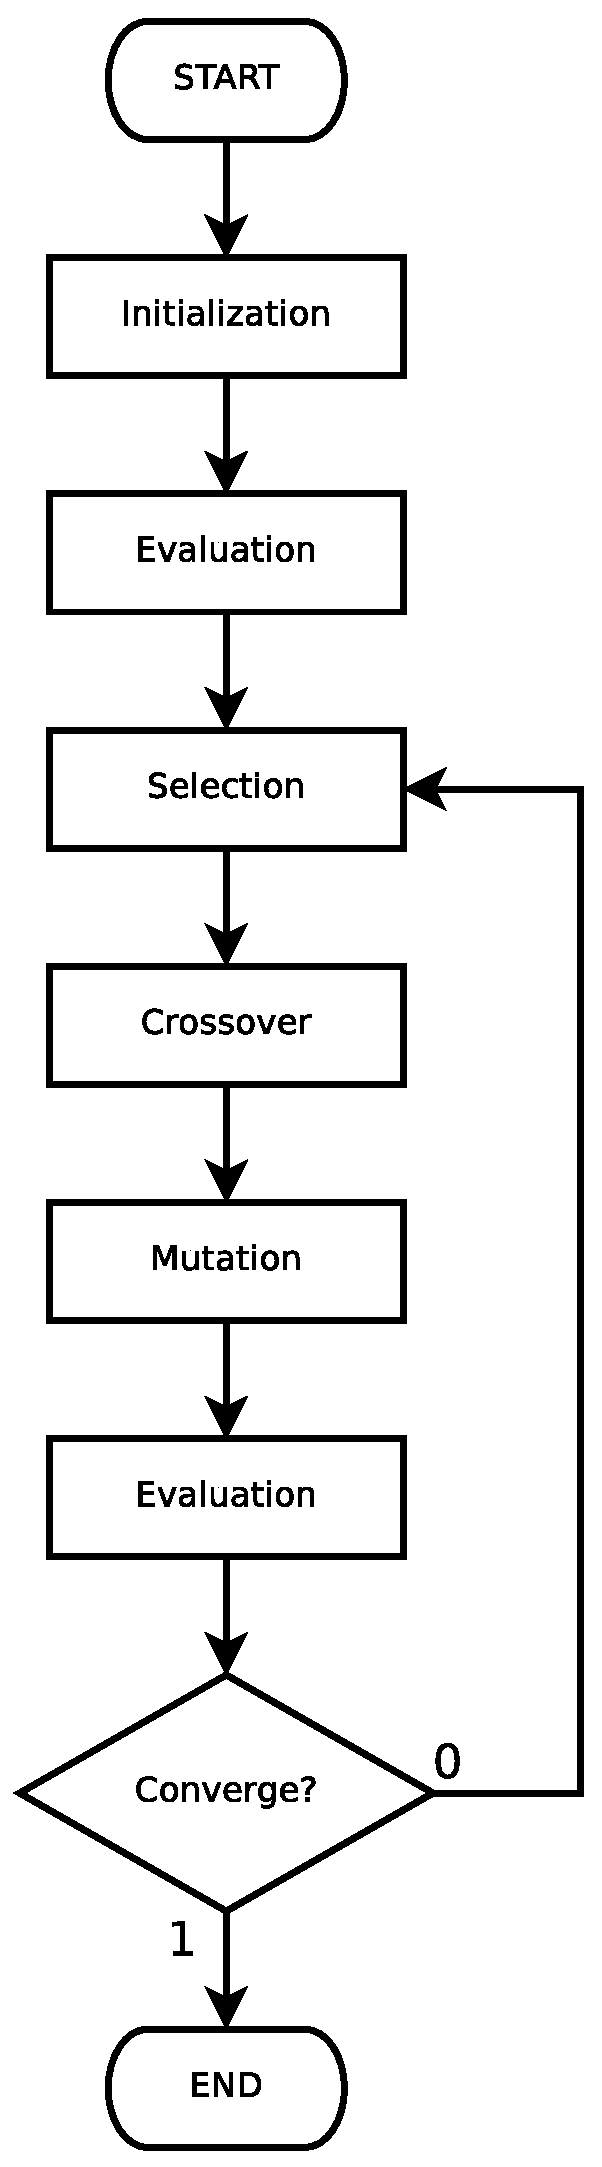
\includegraphics[height=0.65\textheight]{./figures/simple_ga_flow.eps}
	\caption{Traditional Genetic Algorithm Flow Chart}
	\label{fig:simple_GA_flow}
\end{figure}

Subsequent to initialization, each member of the population is evaluated by the
objective function, which is a metric of solution quality or fitness. Thus, an
individual's fitness is represented by the value, or cost, returned by the objective
function evaluation. Individuals are then selected according to their relative fitness for
placement into a mating pool which is a subset of the population. Individuals with a
higher relative fitness have a higher likelihood of selection for mating eligibility while
individuals with a lower relative fitness are more likely to be discarded. Individuals
which have been selected and placed into the mating pool then reproduce via a
crossover operator where reproduction is defined as the random exchange of traits between
selected individuals (progenitors) who produce offspring (progeny) and the crossover
operator is the algorithmic mechanism by which reproduction occurs. Following
reproduction, genetic diversity of the population is generated by introducing new
genetic information into the population via a mutation operator where mutation is defined
as the random alteration of a selected individual's traits.

Each member of the new population, $G_1$, which is now comprised of the mating pool and
their newly generated offspring, is evaluated for fitness. The new generation's
fitness is then analyzed to see if the convergence criteria has been met. If the
convergence criteria has not been met then the population must undergo
selection, reproduction, and mutation again and be reevaluated for convergence. This cycle
continues until the convergence criteria has been met.

%%%%%%%%%%%%%%%%%%%%%%%%%%%%%%%%%%%%%%%%%%%%%%%%
%% 2. HOG algorithm 
%%%%%%%%%%%%%%%%%%%%%%%%%%%%%%%%%%%%%%%%%%%%%%%%%
\section{Hybrid Orthogonal Genetic (HOG) Algorithm}

Figure \ref{fig:HOGA_flow_chart} shows a flow chart of the HOG algorithm which begins by
initializing the population with a random selection of viable solutions, referred to as
individuals or chromosomes. Structurally, each chromosome is represented by a vector of
length $K$ where each element or allele of the vector represents a trait which can be
viewed as genetic information in the chromosome. A population of size
$N$ can be represented by aggregating the chromosomes into a $K\times N$
matrix. Following population initialization, each chromosome is evaluated for fitness
by the objective function. The chromosomes are then sorted and linearly ranked
according to their fitness and selected for placement into a mating pool
according to their relative fitness. Once selected for mating eligibility, pairs of
chromosomes reproduce via a traditional crossover operator producing a pair of offspring.
The offspring and mating pool then reproduce a second time via a hybrid orthogonal
crossover operator. Genetic diversity is then generated through the use of a
mutation operator. Finally, the new generation's fitness is evaluated and the
results are examined for convergence. If convergence conditions are not met then the
process repeats itself until the convergence conditions are satisfied.

\begin{figure}[htbp]
	\centering
	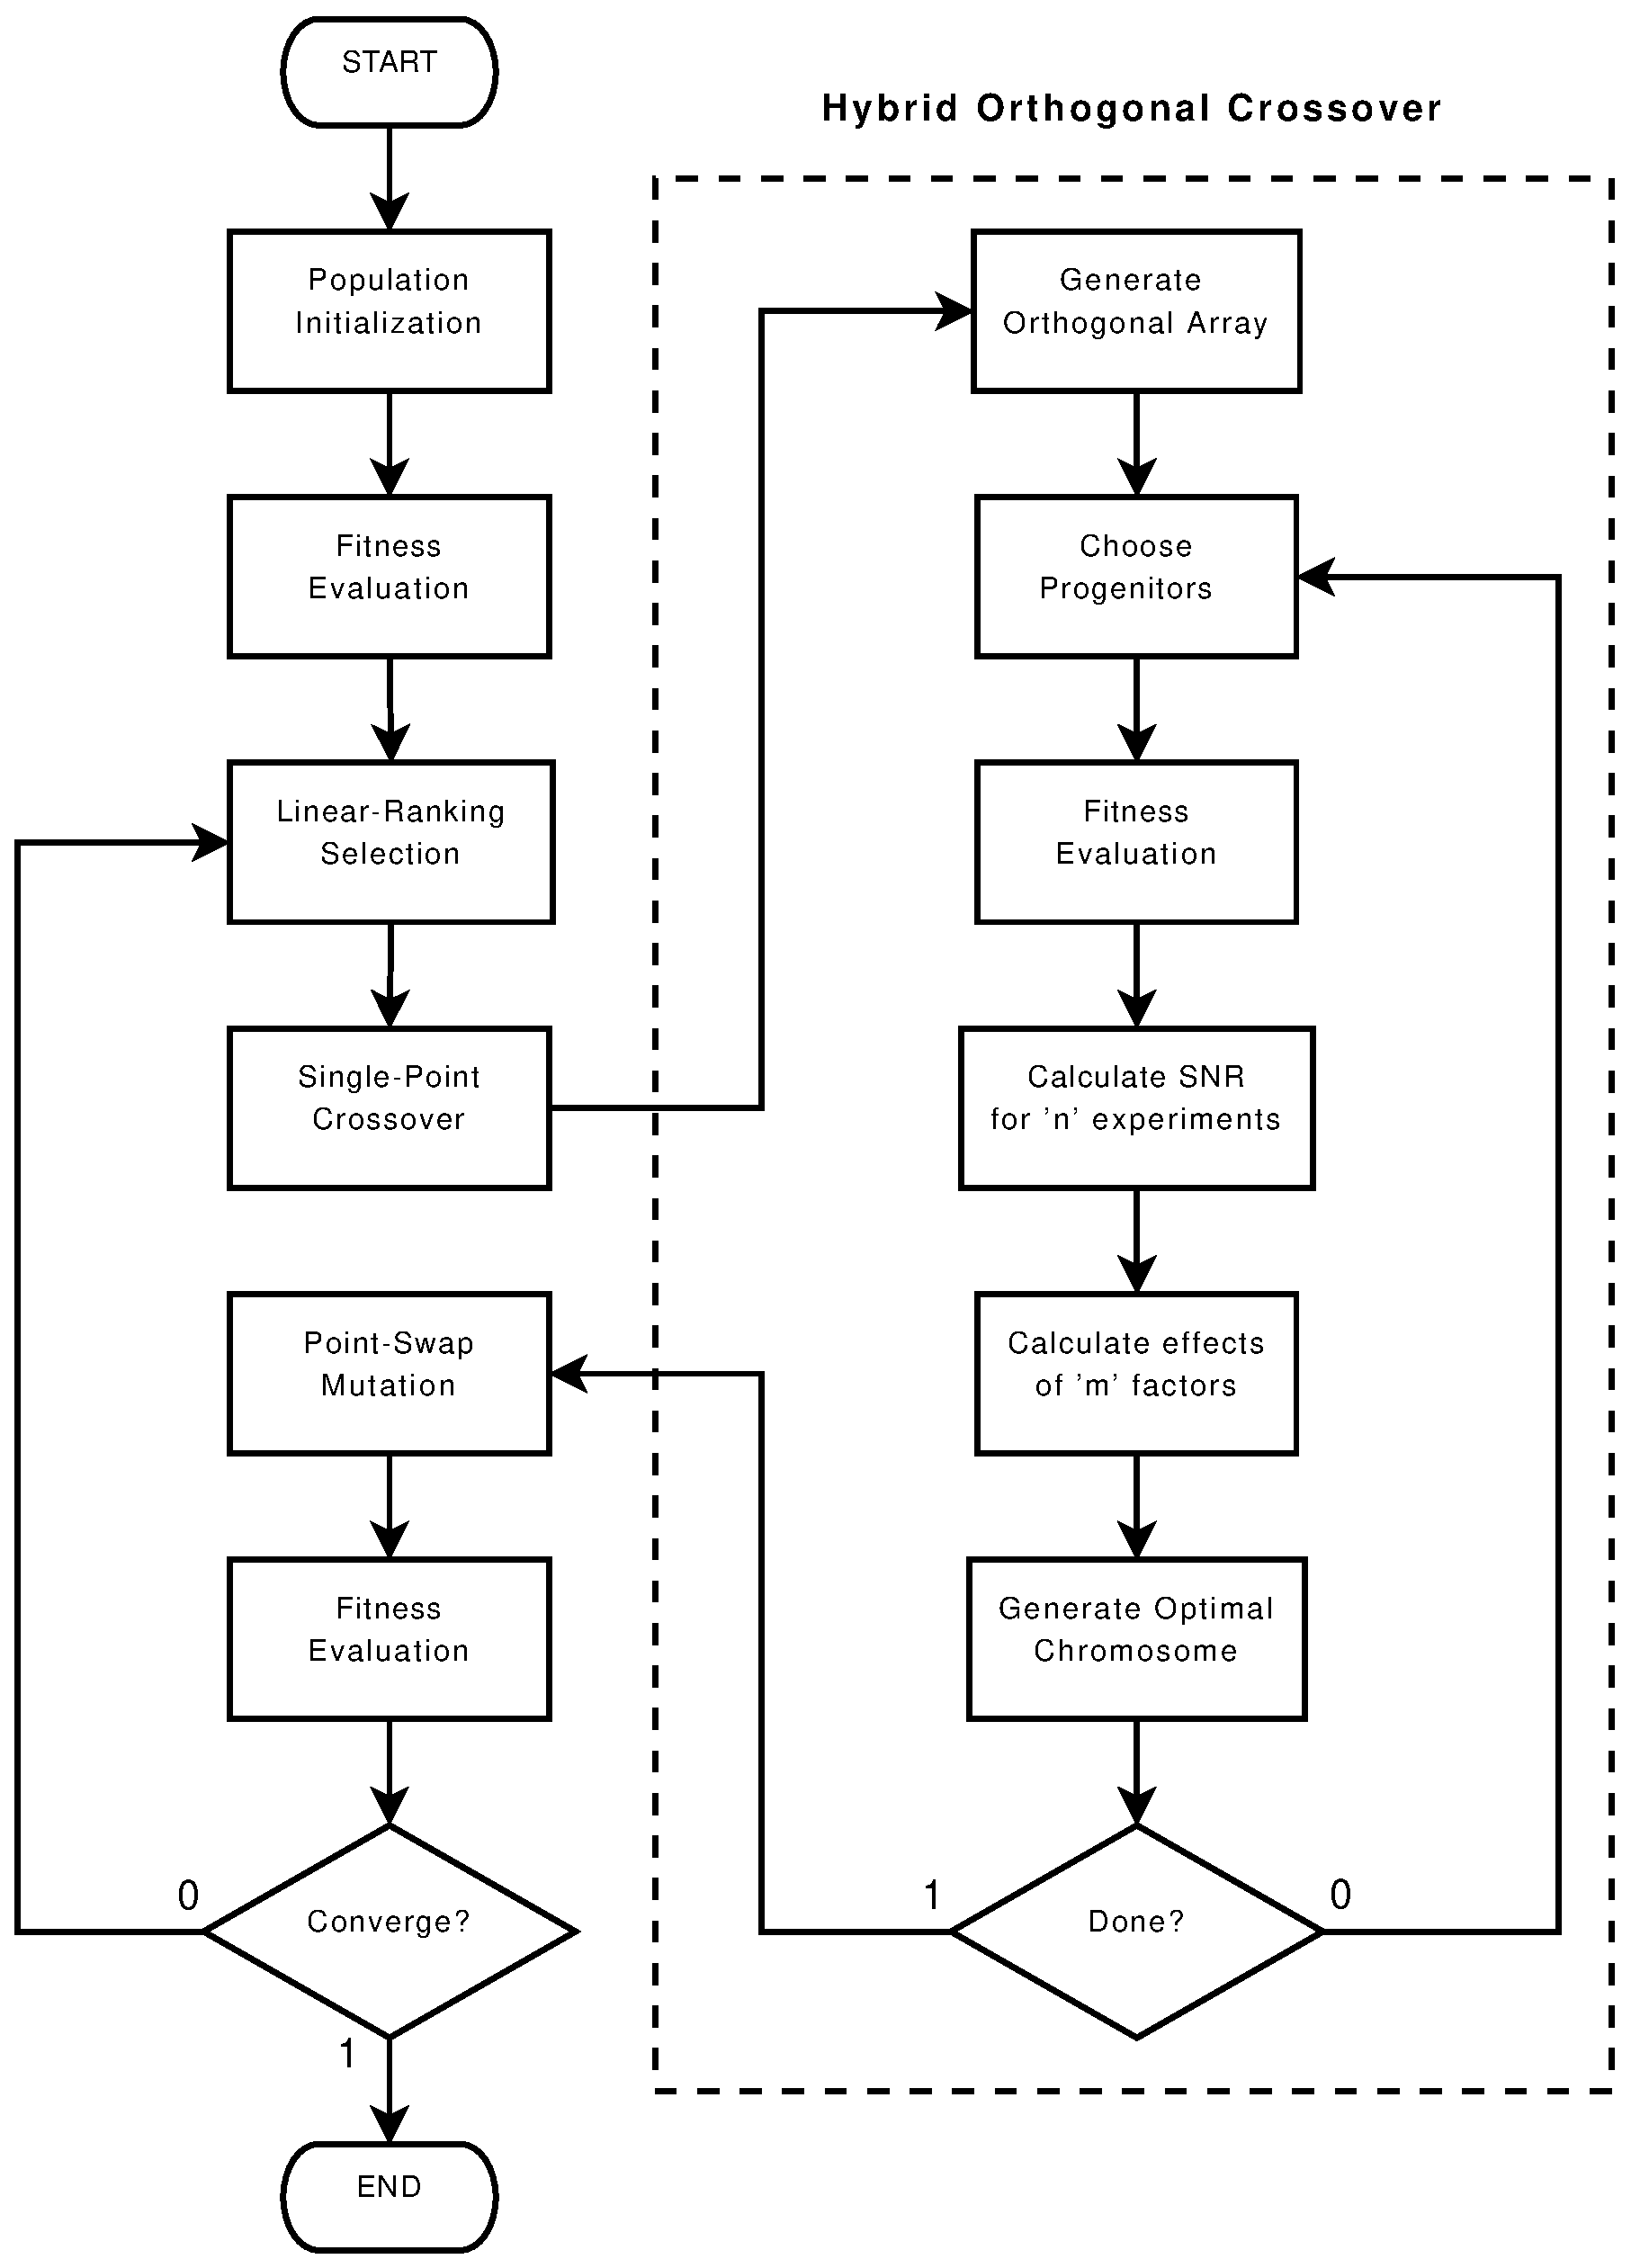
\includegraphics[width=0.9\textwidth]{./figures/HOGA_flow.eps}
	\caption{Hybrid Orthogonal Genetic Algorithm Flow Chart}
	\label{fig:HOGA_flow_chart}
\end{figure}

\subsection{Population Initialization}
In the HOG algorithm, the initial population can be chosen such that the chromosomes are
uniformly distributed over some subset of the solution space. Typically, the initial
population is determined by the nature of the objective function. If the boundaries of
the objective function's feasible solution space are well understood then the initial
population can be selected over the known subset of this feasible solution space.
However, if the boundaries of the feasible solution space are unknown or poorly understood
then it may become necessary to iteratively modify the problem space as knowledge of the
performance surface is gained through trial and error.

\subsection{Fitness Evaluation}
As mentioned previously, the fitness of an individual is determined by evaluating the
objective function for that individual.  Because the HOG algorithm is a minimization based
evolutionary strategy, individuals with lower cost are considered more fit than
individuals with a higher cost. Thus, the HOG algorithm is searching for the individual
$\mathbf{x}$ that satisfies 
%---------------------
\begin{equation}\label{eq:objective_function}
\min_{\mathbf{x}\in\mathbb R^K}\bigl\{J(\mathbf{x})\bigr\}, \quad\mathbf{x}\in S
\end{equation}
%---------------------
where $J(\mathbf{x})$ is the cost or objective function,  $\mathbf{x}$ is a real vector in
$\mathbb{R}^K$, and $S$ is the set of feasible solutions.

\subsection{Linear-Ranking Selection}
 After the individuals in the population are linearly ranked according to their fitness,
each individual is assigned a probability of selection for reproduction such that more fit
individuals have a higher likelihood of reproducing than less fit individuals.
Individuals not selected for reproduction are discarded. In this thesis, the individual
with the best fitness is always selected for mating eligibility ensuring that the most fit
member of any generation is eligible for reproduction. Such algorithms are referred to as
elitist algorithms where elitist is defined as preserving the most fit individual for the
next generation independent from the evolutionary process. The HOG algorithm implements an
elitist, linear-ranking selection scheme to decrease stochastic selection variability and
improve the representation of highly dynamic populations for mating eligibility.

In biological terms, the genotype of a population is defined as the total available
genetic information belonging to that population. The phenotype of a population is defined
as the expressed traits of the population where expression is defined as the observable
display of characteristics related to a particular genetic composition. In evolutionary
systems, phenotypic expression and genotypic content are often very loosely coupled and
extremely difficult to characterize. As such, the observed fitness of an individual
belonging to some population offers only a partial indication of possible reproductive
optimality. Care must be taken that the evolutionary process does not inadvertently
discard the genetic information contained in less-fit individuals which may be required to
achieve the optimal chromosome. Prior to convergence, the optimal chromosome typically
exists as some permutation of traits belonging to individuals which cannot be guaranteed
to have the highest relative fitness. In fact, population dynamics typically exist such
that the relative difference between the most fit and least fit individual is poorly
reflected in its observed fitness even for well formed objective functions
\cite{blickle_comparison_1996}. As such, for most objective functions, the fitness metric
is not a good metric for determining an individual's breeding potential.

To mitigate the statistical selection bias inherent to the objective function, a linear
ranking scheme can be implemented where the population is ordered according to its fitness
prior to selection for mating eligibility \cite{whitley_genitor_89}. In the HOG algorithm,
the population of $N$ individuals is sorted according to their fitness values. Once
sorted, the individuals from the least fit (highest cost) to most fit (lowest cost)
are assigned consecutive integers from 1 to $N$; that is, the least fit individual is
assigned one and the most fit individual is assigned $N$. The probability of selection for
mating eligibility is then assigned according to the individual's rank within the
greater population where the $i$th ranked individual has the probability, $p_i$, of
selection, given as
%---------------------
\begin{equation}\label{eq:linear_ranking}
p_{i}=\frac{1}{N}\biggl(\eta^{-}+\bigl(\eta^{+}-\eta^{-}\bigr)\frac{i-1}{N-1}\biggr)
\end{equation}
%---------------------
where $\bigl(\eta^{-}/N\bigr)$ and $\bigl(\eta^{+}/N\bigr)$ are the probabilities of
selection for the least fit and most fit individual, respectively.
Because the population is comprised of $N$ disjoint elementary events,
%---------------------
\begin{equation}\label{eq:linear_ranking_pdf}
\sum_{i=1}^{N}p_{i}=\sum_{i=1}^{N}\frac{1}{N}\biggl(\eta^{-}+\bigl(\eta^{+}-\eta^{-}
\bigr)\frac{i-1}{N-1}\biggr) = 1\text{.}
\end{equation}
%---------------------
which implies that $\eta^{-}=2-\eta^{+}$ where $0\leq\eta^{+}\leq2$.

Specific selection of $\eta^{-}$ and $\eta^{+}$ allows for control over selection pressure
which is defined as the relationship between the probability of selection of the most fit
vs. least fit individual. It has been shown that fixing $\eta^{+}$ at 1.1 provides an
adequate balance between exploration and exploitation of the performance surface
\cite{back_optimization_1991}.

Because standard operators which rely on stochastic selection where the
probability of selection is proportional to the individual's relative fitness cannot
guarantee that the most fit individuals will be considered for selection and subsequent
reproduction, the possibility exists that good chromosomes may be randomly
discarded. For the HOG algorithm, an elitist selection method is implemented to counter
this phenomenon, where elitism is defined as the process of automatically selecting the
best chromosome(s) for mating eligibility thereby ensuring the availability of their
genetic information for subsequent reproduction. This technique has been shown to greatly
increase convergence speeds, especially for applications where minimizing steady-state
misadjustment is significant \begin{large}                            
\end{large}\cite{reeves_genetic_2002}.

\subsection{Single Point Crossover}
After randomly selecting a group of eligible progenitors, or a mating pool, using the
selection probabilities, randomly paired individuals reproduce by exchanging alleles
where alleles are the elements comprising the vector structure of the chromosome. In
genetic algorithms, this process is referred to as crossover. This sharing of genetic
information is the vehicle by which individuals propagate their beneficial traits.

For both single-point and hybrid orthogonal crossover, pairs of progenitors are randomly
selected from the mating pool and are given the opportunity to exchange genetic
information via the respective crossover operator. Each selected pair is assigned a random
number, $r$ that has a uniform distribution over $\bigl[0,1\bigr]$. Selection for
crossover is governed by the coefficient for crossover probability of, $P_c$, which
typically ranges from 0.2 to 1.0. If $r<P_c$, crossover occurs and genetic information is
exchanged between the pair of progenitors and offspring are produced. Conversely, if
$r\geq P_c$, the pair is returned to the mating pool without producing offspring. Note
that the process by which individuals are randomly selected for crossover is typically
regulated. For this application, self replication is strictly forbidden. Thus,
selected individuals must crossover with a different individual thereby ensuring the
exchange of alleles and preventing a single anomalous individual from inadvertently
dominating the greater population leading the algorithm to converge to a non-optimal
solution.

Recall that reproduction is defined as the exchange of genetic information
between two individuals belonging to a population and that the mechanism of exchange of
vector elements between the individuals is referred to as the crossover operator. Many
different crossover techniques have been analyzed and implemented successfully across a
broad range of objective function types
\cite{poon_genetic_1995}\cite{glover_handbook_2003}. Because the objective function both
characterizes the problem space and evaluates specific chromosomes, the physical structure
of the chromosomes is determined by the characteristics of the objective function.
Thus, the optimal crossover operator is related to the physical structure of the
chromosome. For certain applications, it may be necessary to regulate which alleles can be
exchanged. These regulations are dictated by the relationships which exist between
adjacent groups of alleles. The power of evolutionary strategies lies in achieving a
balance between exploring a solution space and exploiting its localized minima or maxima.
As a result, a balance between preserving the stochastic nature of reproduction and the 
deterministic exchange of genetic information must be maintained. Thus, the
structure of the chromosome should complement the crossover method selected. For the
HOG algorithm, reproduction is achieved by using both a single-point crossover operator
and a hybrid orthogonal crossover operator based on the Taguchi method.

The single-point crossover operator is an arithmetic operator derived from convex set
theory which randomly selects a single crossover point for the selected chromosomes
\cite{jinn-tsong_tsai_hybrid_2004}. For two individuals represented by the real
vectors $\mathcal{C}_\alpha$ and $\mathcal{C}_\beta$, all alleles subsequent to the
crossover point are exchanged between the progenitors and two progeny are created. The
single-point crossover process is illustrated in Figure \ref{fig:crossover} where the
progenitor chromosomes are denoted as $\mathcal{C}_\alpha$ and $\mathcal{C}_\beta$ and the
progeny chromosomes are denoted as $\mathcal{C}_\alpha^\prime$ and
$\mathcal{C}_\beta^\prime$.
%----------------------------
\begin{figure}[H]
\centering
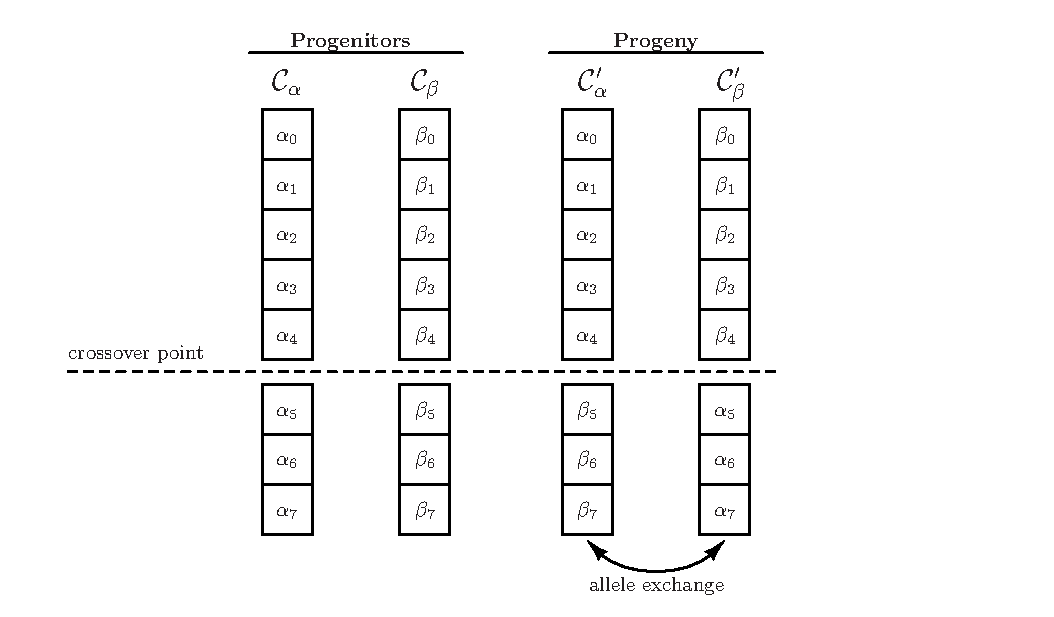
\includegraphics[width=\textwidth]{./figures/crossover.eps}
\caption{Single-Point Crossover}
\label{fig:crossover}
\end{figure}
%----------------------------
Single-point crossover has positional bias in that it favors continuous segments of
genetic information. However, it does not contain distribution bias as the crossover
point  is a discrete random variable with uniform distribution over $\bigl[0,m\bigr]$,
where $m$ denotes the length of the respective chromosome \cite{glover_handbook_2003}.

%%%%%%%%%%%%%%%%%%%%%%%%%%%%%%%%%%%%%%%%%%%%%%%%%%%%%%%%%%%%%%%%%%%%%%%%%%%%%%%%
\subsection{Hybrid Orthogonal Crossover via The Taguchi Method}
After traditional single-point crossover has been performed, the previously selected
mating pool and newly generated progeny undergo an additional exchange of genetic
information using a hybrid crossover technique which intelligently creates more fit
offspring. Unlike the traditional crossover operator, the hybrid orthogonal crossover
operator intelligently draws genetic information from each progenitor to create the best
possible offspring given the traits that are available. Based on the Taguchi method and
using orthogonal-array based experimental design techniques, this method has been shown
to produce the most robust offspring possible given the genetic information available from
the current population \cite{jinn-tsong_tsai_optimal_2006}. It has also been shown to be
significantly less sensitive to ill-formed objective functions and non-linear performance
surfaces and to improve both solution accuracy and overall convergence speed
\cite{jinn-tsong_tsai_hybrid_2004}.

The progenitors are randomly selected from the eligible mating pool as is done 
for the traditional crossover operator. However, unlike traditional crossover operators,
all permutations of possible progeny for a selected pair of progenitors are considered
with the hybrid operator. Each permutation of genetic exchange between the progenitors is
treated as an experiment (trial) where the factors of the experiment correspond to the
available traits. The subsequent fitness evaluation of the progeny can then be treated as
the observation of an experimental trial of $K$ factors where $K$ is
the length of each chromosome
\cite{yiu-wing_leung_orthogonal_2001}\cite{jinn-tsong_tsai_hybrid_2004}. This type of
experiment is commonly referred to as a factorial experiment of $K$ factors. As such,
proven methods from the statistical design of experiments can be used to improve
the experimental process. Specifically, statistical design of experiments is the process
of planning experiments so that significant data can be collected with a minimum number
of performed experiments. Subsequent to data collection, suitable statistical methods are
then used to analyze the collected data and draw statistical inferences accordingly
\cite{shinn-ying_ho_intelligent_2004}.

%%%%%%%%%%%%%%%%%%%%%%%%%%%%%%%%%%%%%%%%%%%%%%%%%%%%%%%%%%%%%%%%%%%%%%%%%%%%%%%%
\subsubsection{Design of Experiments and Orthogonal Arrays}
For a factorial experiment of $K$ factors, there exists $N^K$ trials where $N$ represents
the number of levels for each factor. For the hybrid orthogonal crossover operator, $N=2$
because only two progenitors are available from which to draw traits. Thus, $2^K$
experiments must be performed to determine the most optimal progeny from the
full factorial experiment space where $K$ corresponds to the number of traits
 or experimental factors. Because each permutation must be evaluated by the objective
function to determine the experimental results for that particular trial, performing
all $2^K$ objective function evaluations becomes computationally prohibitive for large
values of $K$. As such, fractional factorial design of experiments can be used to reduce
the number of required experimental trials. The HOG algorithm uses orthogonal array based
design of experiments to reduce the full factorial solution space to a small but
representative number of sample trials\cite{yiu-wing_leung_orthogonal_2001}.

The Taguchi method of design of experiments utilizes two-level orthogonal arrays which are
special arrays derived from the Latin square. An $M$ row and $N$ column Latin square,
denoted as $L_M$, has the form
%---------------------------
\begin{equation}\label{eq:latin_array}
L_{M}\bigl(Q^{N}\bigr) = \bigl[a_{i,j}\bigr]_{M\times
N},\quad a_{i,j}\in\{1,2,\cdots,Q\}
\end{equation}
%---------------------------
where the $M$ rows represent the experimental trials, the $N$ columns
represent the experimental factors, and $Q$ corresponds to the number of levels of
the experimental design\cite{yiu-wing_leung_orthogonal_2001}. Recall that the
hybrid orthogonal crossover operator uses two-level orthogonal arrays. As
such, substituting $Q=2$ into \eqref{eq:latin_array} yields 
%---------------------------
\begin{equation}\label{eq:two_level_array}
L_n\bigl(2^{n-1}\bigr)
\end{equation}
%---------------------------
where $n$ corresponds to the number of trials. The resulting Latin square then represents
an orthogonal set of experiments where orthogonal is defined as the statistical
independence of the columns representing experimental factors. The observations
made over $n$ trials of orthogonal experiments yields the effects of the experimental
factors. In particular, the HOG algorithm uses this information to determine which factors
have the most beneficial contribution to the progeny.

To illustrate, consider an experiment that has 3 factors (alleles) and 2 levels
(progenitors). For this experiment, $2^3$, or 8, unique experiments exist in the full
factorial experiment space.  The Latin square which represents the experimental space is
given as 
%---------------------------
\begin{equation}\label{eq:two_level_array_example}
L_4\bigl(2^{3}\bigr)=
\begin{pmatrix}
1 &1 &1 \\
1 &2 &2 \\
2 &1 &2 \\
2 &2 &1 \\
\end{pmatrix}
\end{equation}
%---------------------------
 which is a 2-level orthogonal array of 4 trials. If the 2's in
\eqref{eq:two_level_array_example} are replaced with -1's, then the inner
product of any two columns of the experimental matrix is null indicating that all
columns of the orthogonal array are mutually orthogonal. Because the columns are
orthogonal the effect of any factor across all trials is statistically independent from
the effect of any other factor \cite{dean_design_2000}. To illustrate, consider 2
progenitors $\mathbf{\alpha}$ and $\mathbf{\beta}$ where $\bm{\alpha}=[ \alpha_1 \quad
\alpha_2 \quad \alpha_3 ]^T$ and $\bm{\beta}=[\beta_1 \quad \beta_2 \quad \beta_3 ]^T$.
Using \eqref{eq:two_level_array_example} to generate the orthogonal experimental matrix,
the corresponding experimental trials and factors are represented by the rows and columns
of Table \ref{tbl:alpha_beta_table} respectively.
%---------------------------
\begin{table}[htpb]
\caption{Two-Level Experimental Matrix for 3 Factors}\label{tbl:alpha_beta_table}
\begin{center}
\begin{tabular}{cccc}
\toprule
Trial ($n$) & \multicolumn{3}{c}{Factors}\\
\midrule
1 & $\alpha_1$ & $\alpha_2$ & $\alpha_3$ \\ 
2 & $\alpha_1$ & $\beta_2$ & $\beta_3$ \\ 
3 & $\beta_1$ & $\alpha_2$ & $\beta_3$ \\
4 & $\beta_1$ & $\beta_2$ & $\alpha_3$ \\ \bottomrule
\end{tabular}
\end{center}
\end{table}
%---------------------------

The Latin square and the full factorial experiment space can be represented
graphically as depicted in Figure \ref{fig:orthogonal_array_plot} where $\phi_x$ represent
the independent factors and the vertices correspond to the space-representative
trials.
%---------------------------
\begin{figure}[htbp]
\centering
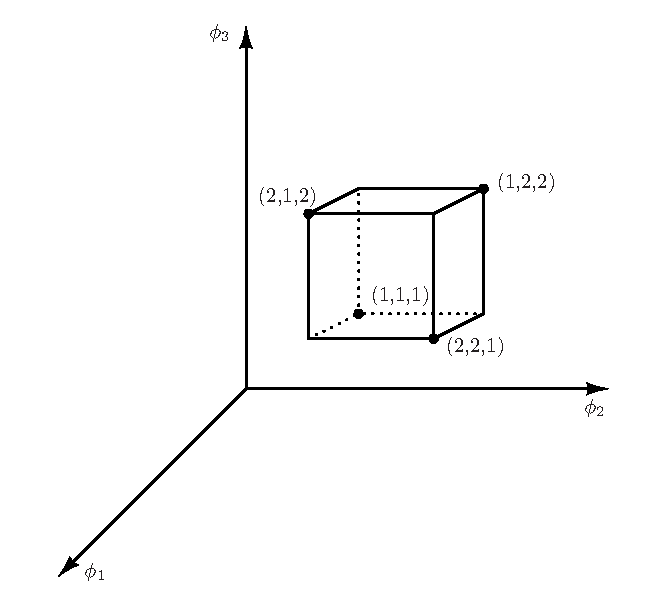
\includegraphics[width=0.6\textwidth]{./figures/orth_array_plot.eps}
\caption{Graphical Representation of $L_{4}\bigl(2^3\bigr)$}
\label{fig:orthogonal_array_plot}
\end{figure}
%---------------------------
As illustrated in Figure \ref{fig:orthogonal_array_plot}, the edges of the graph enclose
the full factorial experiment space. On inspection, it is clear that the full factorial
space of 8 experiments has been reduced to the evaluation of a subset of 4 vertices
thereby decreasing the total number of trials necessary to observe the effects of
the experimental factors by a factor of two.

%%%%%%%%%%%%%%%%%%%%%%%%%%%%%%%%%%%%%%%%%%%%%%%%%%%%%%%%%%%%%%%%%%%%%%%%%%%%%%%%
\subsubsection{Taguchi Method}
To estimate an optimal set of alleles, or factors, from the reduced factorial experiment
space, the Taguchi method determines the cost of each trial of the experimental matrix
and processes these costs in a metric which is used to calculate the observed
effects of all available alleles. Based on this calculation, a set of alleles are selected
from the available progenitors to produce an estimated optimal progeny.

This thesis uses the metric $S_n$ which is defined as the cost
function squared for the $n$th trial, that is, 
%---------------------------
\begin{equation}\label{eq:MSE}
S_n=J^{2}(\bm{x}_n)
\end{equation}
%---------------------------
where $\bm{x}_n$ is a vector containing the alleles, or factors, of the $n$th trial. This
metric is then used to calculate each allele's observed effect which is subsequently
used for determining an estimated optimal progeny.

The observed effect, $E_{x_{k}P_{m}}$, for an allele or factor $x_k$ is defined as the sum
of the metrics, $S_n$, for which the $n$th trial corresponds to the $m$th progenitor's
factor contribution. For example, for the two-level experiment given in Table
\ref{tbl:alpha_beta_table}, the observed effect is given as 
%---------------------------
\begin{equation}\label{eq:effects_of_factors}
 E_{x_{k}P_{m}}=\sum_{i\in \{k:x_k = P_m\}}S_i
\end{equation}
%---------------------------
where $i$ corresponds to the trial number in which the $m$th progenitor $P_m$ contributed
its $k$th respective factor.  For a global minimizer, the optimal contributing $k$th
allele is defined as the allele from the progenitor which gives the lowest value for
$E_{x_{k}P_{m}}$. To illustrate, consider an experiment with two progenitors which
corresponds to a two-level orthogonal array. If $E_{x_{k}P_1} < E_{x_{k}P_2}$ for the
factor $x_k$, the optimal contribution is given by progenitor 1 ($P_1$). Conversely, for
$E_{x _{k}P_1} > E_{x_{k}P_2}$, progenitor 2 ($P_2$) would provide the optimal
contribution \cite{jinn-tsong_tsai_hybrid_2004}. The optimal chromosome is then assembled
by taking the factor from the optimal progenitor for each of the $K$ factors in the
chromosome. This process is further illustrated in the following example.

\subsubsection{Taguchi Method Example}
To illustrate the Taguchi method, consider a cost function $J(\bm{x})$ given as 
%---------------------------
\begin{equation}\label{eq:taguchi_ex_cost_fn}
J(\bm{x})=\sum_{i=1}^{7}x_i^2
\end{equation}
%---------------------------
where $x_1,x_2,\dots,x_7$ are real elements of the vector $\bm{x}$.
Equation \eqref{eq:taguchi_ex_cost_fn} describes an elliptic paraboloid that has a
global minimum at zero.
\sloppy
Consider two randomly selected progenitors, $\mathcal{C}_1$ and $\mathcal{C}_2$, where
$\mathcal{C}_1 = [1 \quad 1 \quad 1 \quad 1 \quad 0 \quad 0 \quad 0]$ and $\mathcal{C}_2 =
[0 \quad 0 \quad 0 \quad 0 \quad 1 \quad 1 \quad 1]$. Because the experiment has 7
factors, or alleles, and 2 progenitors, or levels, the orthogonal array,
$L_{8}\bigl(2^7\bigr)$, where 
%---------------------------
\begin{equation}\label{eq:taguchi_ex_orth_arry}
L_{8}\bigl(2^7\bigr)=
\begin{pmatrix}
1     &1     &1     &1     &1     &1     &1\\
1     &1     &1     &2     &2     &2     &2\\
1     &2     &2     &1     &1     &2     &2\\
1     &2     &2     &2     &2     &1     &1\\
2     &1     &2     &1     &2     &1     &2\\
2     &1     &2     &2     &1     &2     &1\\
2     &2     &1    &1     &2     &2     &1\\
2     &2    &1     &2     &1     &1     &2\\
\end{pmatrix}
\end{equation}
%---------------------------
can be used to form an appropriate experimental matrix. Using the orthogonal array shown
in \eqref{eq:taguchi_ex_orth_arry}, the experimental matrix illustrated in Table
\ref{tbl:taguchi_ex_table} can be created where $n$ denotes the trial number,
$x_k$ denotes the $k$th experimental factor, $\bm{x}_n$ represents the chromosome for
the $n$th trial, $J(\bm{x}_n)$ corresponds to the evaluated cost for the $n$th
experimental trial, and $S_n$ corresponds to the calculated metric for the $n$th
experimental trial.
%---------------------------
\begin{table}[htbp]
\begin{center}
 \caption{Taguchi Method Example Experimental Matrix}\label{tbl:taguchi_ex_table}
 \begin{tabular}{ccccccccccc}\toprule
\multirow{2}*{Trial ($n$)} &
\multirow{2}*{Chromosome} &
\multicolumn{7}{c}{Experimental Factors} & 
\multirow{2}*{$J_{n}(\bm{x}_n)$} &
\multirow{2}*{$S_n$} \\ 
&
&
$x_1$ &
$x_2$ &
$x_3$ &
$x_4$ &
$x_5$ &
$x_6$ &
$x_7$ & \\ \midrule 
1 & $\bm{x}_1$ & 1 & 1 & 1 & 1 & 0 & 0 & 0 & 4 & 16 \\ 
2 & $\bm{x}_2$ & 1 & 1 & 1 & 0 & 1 & 1 & 1 & 6 & 36\\ 
3 & $\bm{x}_3$ & 1 & 0 & 0 & 1 & 0 & 1 & 1 & 4 & 16\\ 
4 & $\bm{x}_4$ & 1 & 0 & 0 & 0 & 1 & 0 & 0 & 2 & 4\\ 
5 & $\bm{x}_5$ & 0 & 1 & 0 & 1 & 1 & 0 & 1 & 4 & 16\\ 
6 & $\bm{x}_6$ & 0 & 1 & 0 & 0 & 0 & 1 & 0 & 2 & 4\\ 
7 & $\bm{x}_7$ & 0 & 0 & 1 & 1 & 1 & 1 & 0 & 4 & 16\\ 
8 & $\bm{x}_8$ & 0 & 0 & 1 & 0 & 0 & 0 & 1 & 2 & 4\\ \bottomrule
\end{tabular}
\end{center}
\end{table}
%---------------------------

Table \ref{tbl:taguchi_ex_table} provides all the necessary information to calculate the
observed effects, $E_{x_{k}P_{m}}$, for the $K$ alleles which are available from the two
progenitors $P_1$ and $P_2$. For this example, the observed effects are calculated as
follows:
%---------------------------
\begin{align*}
%--------------------------- P_1(x_1) = 1 --- P_2(x_1) = 0
&E_{x_1 P_1}=\sum_{i\in\{n:x_1 = 1\}=\{1,2,3,4\}}S_i=72 &\quad
&E_{x_1 P_2}=\sum_{i\in\{n:x_1 = 0\}=\{5,6,7,8\}}S_i=40\\
%--------------------------- P_1(x_1) = 1 ---  P_2(x_1) = 0
&E_{x_2 P_1}=\sum_{i\in\{n:x_2 = 1\}=\{1,2,5,6\}}S_i=72 &\quad
&E_{x_2 P_2}=\sum_{i\in\{n:x_2 = 0\}=\{3,4,7,8\}}S_i=40\\
%--------------------------- P_1(x_1) = 1 ---  P_2(x_1) = 0 
&E_{x_3 P_1}=\sum_{i\in\{n:x_3 = 1\}=\{1,2,7,8\}}S_i=72 &\quad
&E_{x_3 P_2}=\sum_{i\in\{n:x_3 = 0\}=\{3,4,5,6\}}S_i=40\\
%--------------------------- P_1(x_1) = 0 ---  P_2(x_1) = 1
&E_{x_4 P_1}=\sum_{i\in\{n:x_4 = 0\}=\{1,3,5,7\}}S_i=64 &\quad
&E_{x_4 P_2}=\sum_{i\in\{n:x_4 = 1\}=\{2,4,6,8\}}S_i=48\\
%--------------------------- P_1(x_1) = 0 ---  P_2(x_1) = 1
&E_{x_5 P_1}=\sum_{i\in\{n:x_5 = 0\}=\{1,3,6,8\}}S_i=40 &\quad
&E_{x_5 P_2}=\sum_{i\in\{n:x_5 = 1\}=\{2,4,5,7\}}S_i=72\\
%--------------------------- P_1(x_1) = 0 ---  P_2(x_1) = 1
&E_{x_6 P_1}=\sum_{i\in\{n:x_6 = 0\}=\{1,4,5,8\}}S_i=40 &\quad
&E_{x_6 P_2}=\sum_{i\in\{n:x_6 = 1\}=\{2,3,6,7\}}S_i=72\\
%--------------------------- P_1(x_1) = 0 ---  P_2(x_1) = 1
&E_{x_7 P_1}=\sum_{i\in\{n:x_7 = 0\}=\{1,4,6,7\}}S_i=40 &\quad
&E_{x_7 P_2}=\sum_{i\in\{n:x_7 = 1\}=\{2,3,5,8\}}S_i=72
%---------------------------
\end{align*}
%---------------------------
The estimated optimal chromosome, $\mathcal{C}^*$, is given as 
\begin{equation}\label{eq:optimal_chromosome}
 \mathcal{C}^*=[x_1^*,x_2^*,\dots,x_k^*]
\end{equation}
where $x_k^*$ represents the optimal $k$th allele. For example, because $E_{x_1 P_2} <
E_{x_1 P_1}$, the first optimal allele is given as $x_1^*= 0$ which corresponds to the
first allele of the second progenitor ($P_2$). The remaining results are summarized in
Table \ref{tbl:taguchi_results_table}. Based on these results, the estimated optimal
chromosome is given as $\mathcal{C}^*= [0 \quad 0 \quad 0 \quad 0 \quad 0 \quad 0 \quad
0]$. Evaluating $\mathcal{C}^*$ by \eqref{eq:taguchi_ex_cost_fn} yields a result
of zero verifying that the result is globally optimal.
%---------------------------
\begin{table}[htbp]
\begin{center}
 \caption{Taguchi Method Example Results}\label{tbl:taguchi_results_table}
 \begin{tabular}{lccccccccc}\toprule
\multirow{2}*{\textbf{Description}}&
\multirow{2}*{\textbf{Expression}}&
&
\multicolumn{7}{c}{\textbf{Experimental Factors}} \\
& & & 
$x_1$ &
$x_2$ &
$x_3$ &
$x_4$ &
$x_5$ &
$x_6$ &
$x_7$ \\ \midrule
\multirow{2}*{Observed Effects} &
$E_{x_k P_1}$    & & 72 & 72 & 72 & 64 & 40 & 40 & 40 \\ 
& $E_{x_k P_2}$    & & 40 & 40 & 40 & 48 & 72 & 72 &72  \\  \midrule
Chromosome 1  & $\mathcal{C}_1$ & & 1 & 1 & 1 & 1 & 0 & 0 & 0 \\
Chromosome 2 & $\mathcal{C}_2$ & & 0 & 0 & 0 & 0 & 1 & 1 & 1 \\
Optimal Progenitor &
--& & 
$\mathcal{C}_2$ &
$\mathcal{C}_2$ & 
$\mathcal{C}_2$ & 
$\mathcal{C}_2$ & 	
$\mathcal{C}_1$ &
$\mathcal{C}_1$ & 
$\mathcal{C}_1$ \\ \midrule
Optimal Progeny & 
$\mathcal{C}^*$ & &
0 & 0 & 0 & 0 & 0 & 0 & 0 \\ \bottomrule
\end{tabular}
\end{center}
\end{table}
%---------------------------

%%%%%%%%%%%%%%%%%%%%%%%%%%%%%%%%%%%%%%%%%%%%
%%% Point-Swap Mutation
\subsection{Single Point-Swap Mutation}
Whether stochastic or guided via the Taguchi method, the process of transferring genetic
information between members of any given population through crossover potentially
evolves more fit individuals from the currently available genotype. The genetic
composition of the more fit offspring is limited by the genetic diversity within
the current generational genotype. If the optimal chromosome is to be evolved through
crossover alone, the optimal genes must exist within the genotype. Because this cannot be
guaranteed, a single-point mutation operator is implemented to introduce new genetic
information into the otherwise static genotype. This process is illustrated in Figure
\ref{fig:mutation}.
%----------------------------
\begin{figure}[H]
\centering
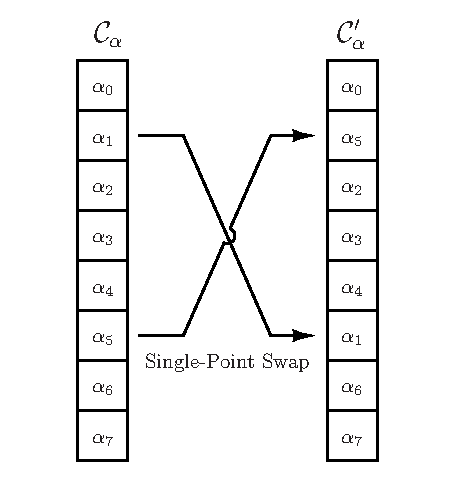
\includegraphics[width=0.4\textwidth]{./figures/single_point_mutation.eps}
\caption{Single-Point Swap Mutation}
\label{fig:mutation}
\end{figure}
%----------------------------
Each individual is assigned a random number $s$ that has a uniform distribution over
$\bigl[0,1\bigr]$. Similar to crossover, mutation is governed by a coefficient for
probability of mutation, $P_m$, which typically ranges from 0.01 to 0.1. If $s<P_m$,
mutation occurs and genetic diversity is introduced through single point-swap mutation.
Conversely, if $s\geq P_m$, the individual is returned to the population unaltered.
For this thesis, the best or elite chromosome is also eligible for mutation,
thereby avoiding premature convergence and increasing the robust nature of the algorithm.

%%%%%%%%%%%%%%%%%%%%%%%%%%%%%%%%%%%%%%%%%%%%
%%% Convergence
\subsection{Convergence}
Convergence is characterized by a stall in evolutionary progress which can be detected
by a lack of improvement of objective function performance over some number of
generations of the best chromosome. The stochastic introduction of new genetic information
via the mutation operator ensures that there will always be some steady state
misadjustment. However, the elitist nature of the algorithm ensures that the best
chromosome a member of the mating pool.

Because the selection operator favors the most fit individuals, the population
will converge to the most fit individual as evolutionary stall persists. As such,
another method for detecting convergence is to compare the population variance against a
threshold value. Both methods have been used in the development of the HOG algorithm.
However, it
was observed that selecting a minimum of 1000 generations and a stall of 50 generations
was sufficient for determining convergence in most cases which is
consistent with results shown in \cite{yiu-wing_leung_orthogonal_2001}.

%%%%%%%%%%%%%%%%%%%%%%%%%%%%%%%%%%%%%%%%%%%%%%%%%
%% 3. Example
%%%%%%%%%%%%%%%%%%%%%%%%%%%%%%%%%%%%%%%%%%%%%%%%%
\subsection{HOG Algorithm Application Examples}
To demonstrate the HOG algorithm, three different cost functions were
selected which are considered canonical exercises for determining the
robustness of optimization algorithms
\cite{price_differential_2005}\cite{yiu-wing_leung_orthogonal_2001}\cite{
jinn-tsong_tsai_hybrid_2004}.

\subsubsection{Example 1: MATLAB\textsuperscript{\textregistered} Peaks Function}
The MATLAB\textsuperscript{\textregistered} \textit{Peaks} function, denoted as $P(x,y)$,
where
%----------------------------
\begin{equation}\label{eq:peaks_function}
 P(x,y)=3\bigl(1-x\bigr)^2
e^{\left(-x^{2}-\left(y+1\right)^{2}\right)}-10\Bigl(\frac{x}{5}-x^{3}-y^{5}\Bigr)e^
{\left(-x^{2}-y^{2}\right)}-\frac{1}{3}e^{\left(-\left(x+1\right)^{2}-y^{2}\right)}
\end{equation}
%----------------------------
and $x$ and $y$ are real continuous variables is a function that is obtained by
translating and scaling Gaussian distributions. The \textit{Peaks} function in
\eqref{eq:peaks_function} exhibits two local minima and one global minimum near
$(0.25,-1.625)$ as illustrated in Figure \ref{fig:peaks}.
%----------------------------
\begin{figure}[htpb]
	\centering
	\includegraphics[width=\textwidth]{./figures/peaks_surf.eps}
	\caption{MATLAB\textsuperscript{\textregistered} \textit{Peaks} Function}
	\label{fig:peaks}
\end{figure}
%----------------------------

\paragraph{Algorithm Setup and Initialization}
To find the global minimum of the  the \textit{Peaks} function, the HOG algorithm
was initially configured with a population size of 200 chromosomes. The $n$th chromosome
was seeded with two alleles, $x_n$ and $y_n$, where $x_n$ and $y_n$ are continuous random
variables uniformly distributed over the feasible solution space,
$\left\{(x,y):-3\leq x\leq3,-3\leq y\leq3\right\}$. To illustrate
average performance metrics, the HOG algorithm was applied 50 times to minimizing the cost
function given in \eqref{eq:peaks_function}. For each trial, convergence was defined as a
lack of further improvement over 50 successive generations following a minimum of 1000
generations. The remaining HOG algorithm parameters are summarized in Table
\ref{tbl:peaks_setup}.
%----------------------------
\begin{table}[htbp]
 \begin{center}
 \caption[MATLAB\textsuperscript{\textregistered} \textit{Peaks} Function Minimization:
Algorithm Parameters]{MATLAB\textsuperscript{\textregistered} \textit{Peaks} Function
Minimization:
HOG Algorithm Parameters}
 \label{tbl:peaks_setup}
 \begin{tabular}{ l c }\toprule
 \textbf{Description} & \textbf{Value} \\ \midrule
Problem Dimension & 2 \\
Population Size & $200 \times 2$ \\
Feasible Solution Space & $-3\leq \{x_n,y_n\}\leq3$ \\
Probability of Crossover & $P_c = 0.2$ \\
Probability of Mutation & $P_m = 0.02$ \\
Selection Pressure & $\eta^+ = 1.1$\\ \bottomrule
\end{tabular}
\end{center}
\end{table}


\paragraph{Results}
In all 50 cases, the HOG algorithm successfully reached the global minimum. Figure
\ref{fig:peaks_learning_curve} illustrates the average learning curve over all 50 runs of
the HOG algorithm when applied to the \textit{Peaks} function.
%----------------------------
\begin{figure}[H]
	\centering
	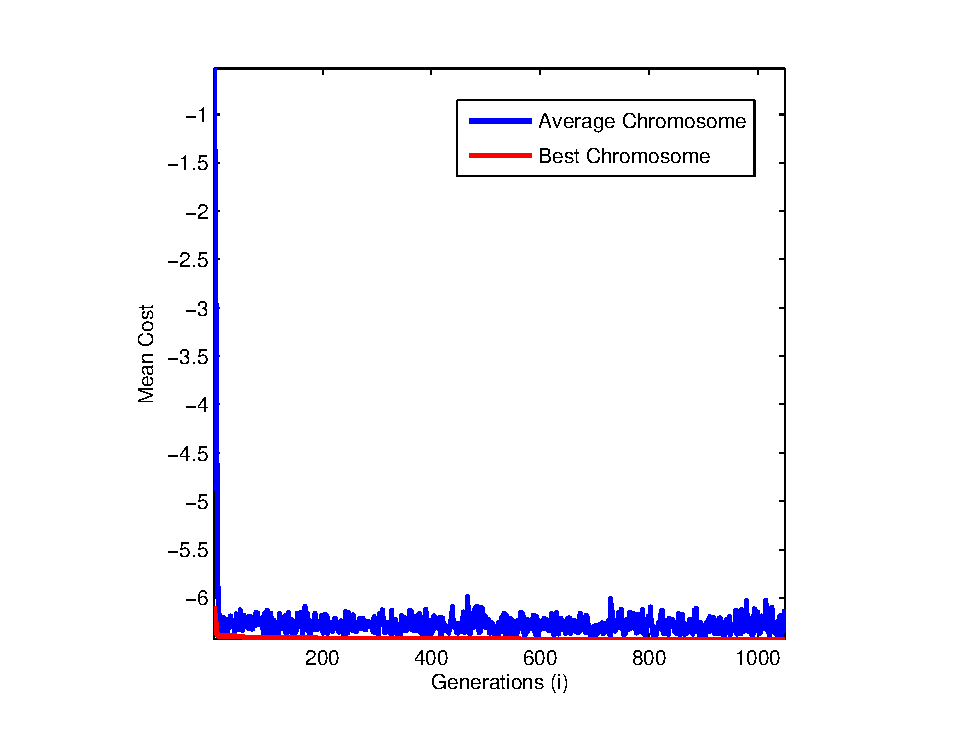
\includegraphics[width=0.8\textwidth]{./figures/peaks_learning_curve.eps}
	\caption{MATLAB\textsuperscript{\textregistered} \textit{Peaks} Function
Minimization: Average Cost}
	\label{fig:peaks_learning_curve}
\end{figure}
%----------------------------
Figure \ref{fig:peaks_descent} shows a parametric plot of the \textit{Peaks} function and
plots the average chromosome for each generation of a population for one of the 50 cases.
Figure \ref{fig:peaks_descent} shows that the average chromosome converges to the optimum
value located at the global minimum of 6.5 at $(x,y)=(0.25,-1.625)$.
%----------------------------
\begin{figure}[H]
	\centering	
	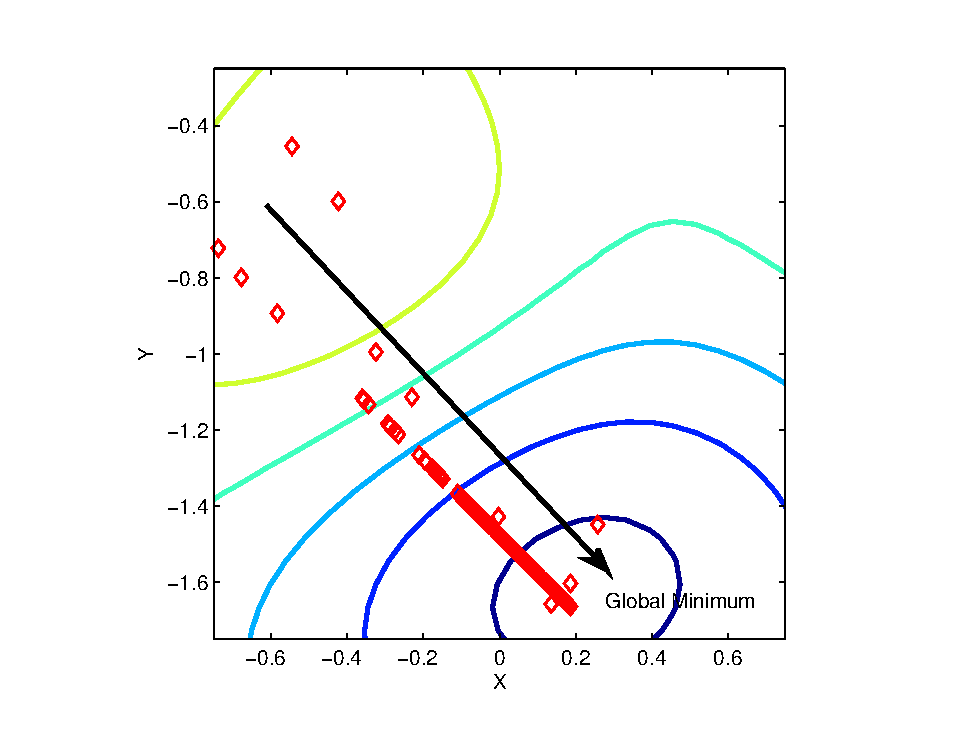
\includegraphics[width=0.8\textwidth]{./figures/peaks_descent.eps}
	\caption[MATLAB\textsuperscript{\textregistered} \textit{Peaks} Function
Minimization: Parametric Plot]{MATLAB\textsuperscript{\textregistered} \textit{Peaks}
Function
Minimization: Average Chromosome
	Parametric Plot}
	\label{fig:peaks_descent}
\end{figure}
%----------------------------

\subsubsection{Example 2: Rastrigin Function}
The Rastrigin function is a highly multimodal nonlinear function that is often used to
test global optimizers and specifically genetic algorithms. The Rastrigin function,
$f(\bm{x})$ is defined as
%----------------------------
\begin{equation}\label{eq:rastigrin}
f(\bm{x}) = \sum_{i=1}^{N}\Bigl[x_{i}^2-10\cos\bigl(2\pi x_i\bigr)+10\Bigr]
\end{equation}
%----------------------------
and the two dimensional case is plotted in Figure \ref{fig:rast_surf}. As illustrated in
Figure \ref{fig:rast_surf}, the two dimensional Rastrigin function is characterized by its
numerous local minima
and a global minimum at $(0,0)$.
%----------------------------
\begin{figure}[H]
	\centering
	\includegraphics[width=\textwidth]{./figures/rast_surf.eps}
	\caption{Two-Dimensional Rastrigin Function}
	\label{fig:rast_surf}
\end{figure}

\paragraph{Algorithm Setup and Initialization}
To find the global minimum of the the Rastrigin function, the HOG algorithm was
configured with a population size of 200 chromosomes. Each chromosome was seeded with
two alleles, $x_{1n}$ and $x_{2n}$, where $x_{1n}$ and $x_{2n}$ are continuous random
variables which are uniformly distributed over the feasible solution space,
$\left\{(x_1,x_2):-5.12\leq x_1\leq5.12,-5.12\leq x_2\leq5.12\right\}$. To
illustrate average performance metrics, the HOG algorithm was applied 50 times to
minimizing the cost function given in \eqref{eq:rastigrin}. For each trial, convergence
was defined as a lack of further improvement over 50 successive generations following a
minimum of 1000 generations. The remaining HOG algorithm parameters are summarized in
Table \ref{tbl:rast_setup}.
%----------------------------
\begin{table}[htbp]
 \begin{center}
 \caption[Rastrigin Function Minimization: Algorithm
Parameters]{Rastrigin Function Minimization: HOG Algorithm
Parameters}\label{tbl:rast_setup}
 \begin{tabular}{ l c }\toprule
 \textbf{Description} & \textbf{Value} \\ \midrule
Problem Dimension & 2 \\
Population Size & $200 \times 2$ \\
Feasible Solution Space & $-5.12\leq \{x_n,y_n\}\leq5.12$ \\
Probability of Crossover & $P_c = 0.2$ \\
Probability of Mutation & $P_m = 0.02$ \\
Selection Pressure & $\eta^+ = 1.1$\\ \bottomrule
\end{tabular}
\end{center}
\end{table}

\paragraph{Results}
In all 50 cases, the HOG algorithm successfully reached the global minimum. Figure
\ref{fig:rast_learning_curve} illustrates the average learning curve over all 50 runs of
the HOG algorithm when applied to the Rastrigin function.
%----------------------------
\begin{figure}[htbp]
	\centering
	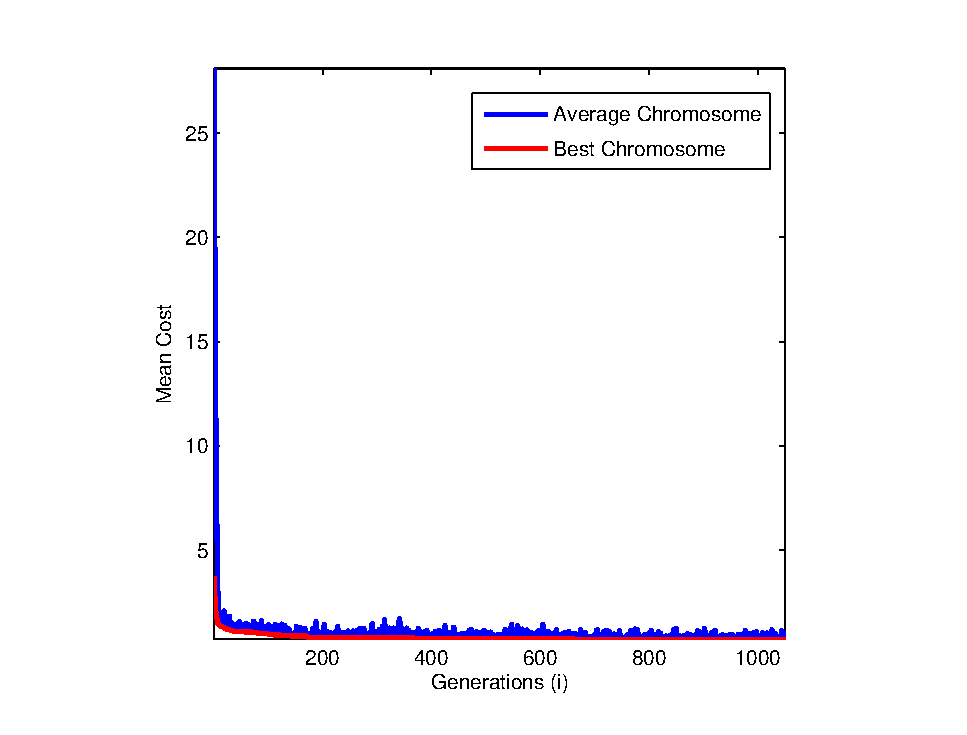
\includegraphics[width=0.8\textwidth]{./figures/rast_learning_curve.eps}
	\caption{Rastrigin Function Minimization: Average Cost}
	\label{fig:rast_learning_curve}
\end{figure}
%----------------------------

Figure \ref{fig:rast_descent} shows a parametric plot of the Rastrigin function and plots
the average chromosome for each generation of a population for one of the 50
cases. As indicated by the arrows, the algorithm initially finds a local minima
adjacent to the global minimum. However, the average chromosome converges to the
global optimum value located at $(0,0)$.
%----------------------------
\begin{figure}[htbp]
	\centering
	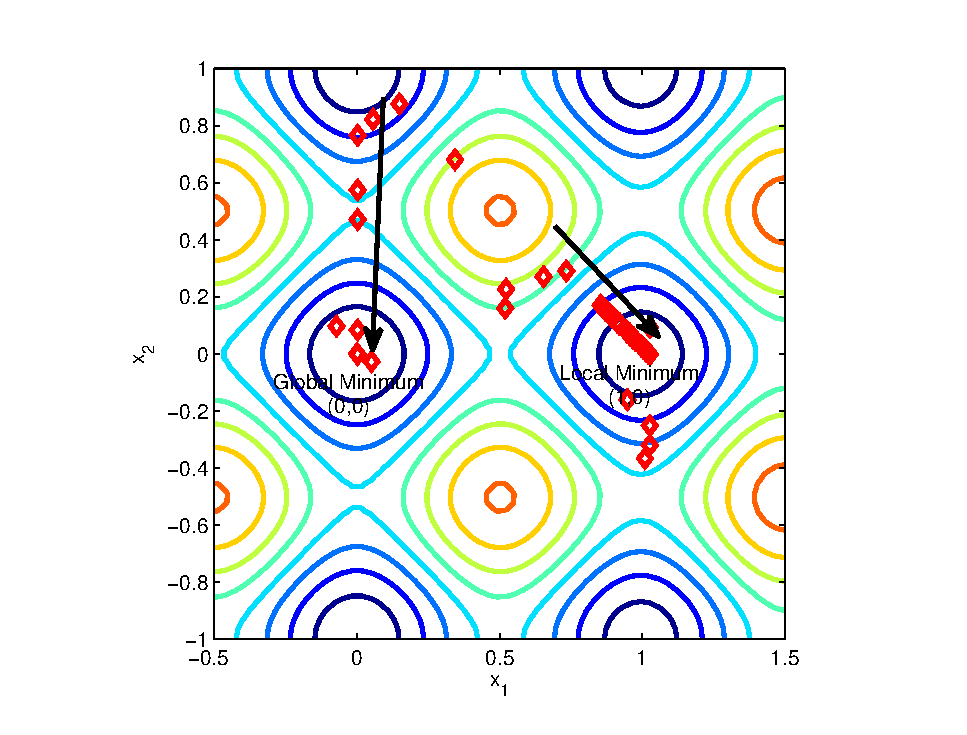
\includegraphics[width=0.8\textwidth]{./figures/rast_descent.eps}
	\caption[Rastrigin Function Minimization: Parametric
Plot]{Rastrigin Function Minimization:
Average Chromosome Parametric
Plot}
	\label{fig:rast_descent}
\end{figure}

\subsubsection{Example 3: Rosenbrock Function}
The Rosenbrock function is a uni-modal non-linear function often used to evaluate the
performance of optimization algorithms. The Rosenbrock function, $f(\bm{x})$, is defined
as
%----------------------------
\begin{equation}\label{eq:rosenbrock}
f(\bm{x}) = \sum_{i=1}^{N-1}\Bigl[\bigl(1-x_i\bigr)^2+ 100 \bigl(x_{i+1} - x_i^2 \bigr)^2
\Bigr]
\end{equation}
%----------------------------
and the two dimensional case is plotted in Figure \ref{fig:rose_surf}. As illustrated in
Figure \ref{fig:rose_surf}, the two dimensional Rosenbrock function is characterized by
its long banana shaped valley with a global minimum at $(1,1)$.
\begin{figure}[htbp]
	\centering
	\includegraphics[width=\textwidth]{./figures/rose_surf.eps}
	\caption{Two-Dimensional Rosenbrock Function}
	\label{fig:rose_surf}
\end{figure}

\paragraph{Algorithm Setup and Initialization}
To find the global minimum of the the Rosenbrock function, the HOG algorithm was
configured with a population size of 200 chromosomes. The $n$th chromosome was seeded with
two alleles, $x_{1n}$ and $x_{2n}$, where $x_{1n}$ and $x_{2n}$ are continuous random
variables which are uniformly distributed over the feasible solution space,
$\left\{(x_1,x_2):-\pi\leq x_1 \leq\pi,-\pi\leq x_2\leq\pi\right\}$. To illustrate
average performance metrics, the HOG algorithm was applied 50 times to minimizing the cost
function given in \eqref{eq:rosenbrock}. For each trial, convergence was defined as a
lack of further improvement over 50 successive generations following a minimum of 1000
generations. The remaining HOG algorithm parameters are summarized in Table
\ref{tbl:rose_setup}.
%----------------------------
\begin{table}[htbp]
 \begin{center}
 \caption[Rosenbrock Function Minimization: Algorithm Parameters]{Rosenbrock Function
Minimization: HOG Algorithm Parameters}
 \label{tbl:rose_setup}
 \begin{tabular}{ l c }\toprule
 \textbf{Description} & \textbf{Value} \\ \midrule
Problem Dimension & 2 \\
Population Size & $200 \times 2$ \\
Feasible Solution Space & $-\pi\leq \{x_n,y_n\}\leq\pi$ \\
Probability of Crossover & $P_c = 0.2$ \\
Probability of Mutation & $P_m = 0.02$ \\
Selection Pressure & $\eta^+ = 1.1$\\ \bottomrule
\end{tabular}
\end{center}
\end{table}

\paragraph{Results}
In all 50 cases, the HOG algorithm successfully reached the global minimum. Figure
\ref{fig:rose_learning_curve} illustrates the average learning curve over all 50 runs of
the HOG algorithm when applied to the Rosenbrock function.
%----------------------------
\begin{figure}[htbp]
	\centering
	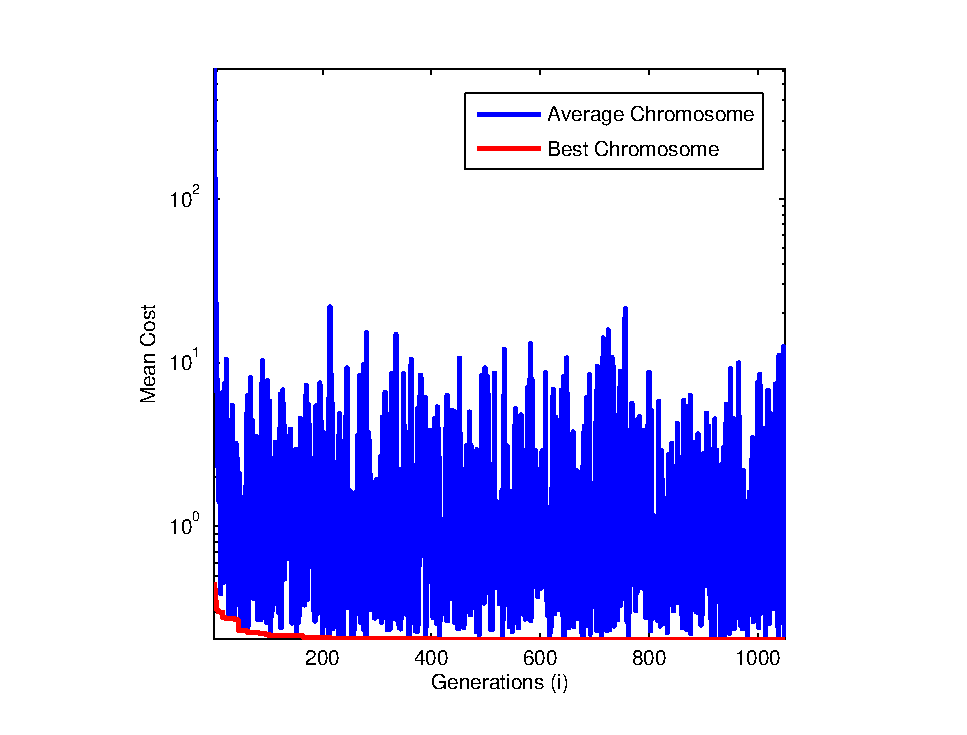
\includegraphics[width=0.8\textwidth]{./figures/rose_learning_curve.eps}
	\caption{Rosenbrock Function Minimization: Average Cost}
	\label{fig:rose_learning_curve}
\end{figure}
%----------------------------

Figure \ref{fig:rose_descent} shows a parametric plot of the Rosenbrock function
and plots the average chromosome for each generation of a population for one of the 50
cases. Figure \ref{fig:rose_descent} shows that the average chromosome converges to the
optimum value located at the global minimum $(1,1)$.
%----------------------------
\begin{figure}[htbp]
	\centering
	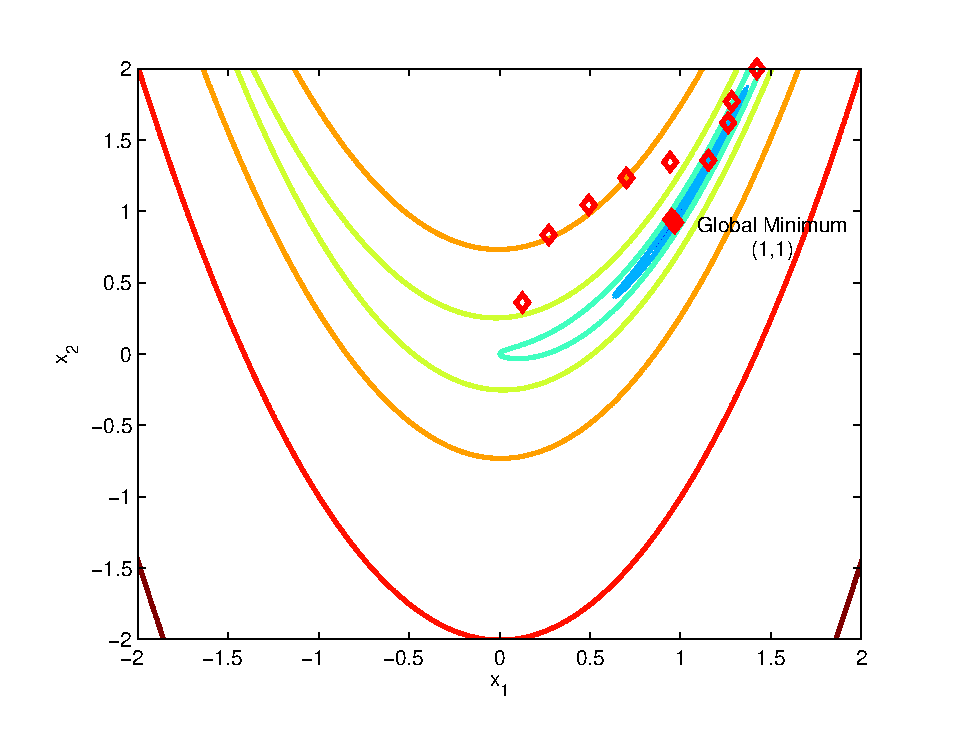
\includegraphics[width=0.8\textwidth]{./figures/rose_descent.eps}
	\caption[Rosenbrock Function Minimization: Parametric
	Plot]{Rosenbrock Function Minimization: Average Chromosome Parametric
	Plot}	
	\label{fig:rose_descent}
\end{figure}

% CHAPTER 4: DSM DESIGN IMPLEMENTAION AND RESULTS
\chapter{Implementation and Results}
\label{ch:Implementation and Results}
%%%%%%%%%%%%%%%%%%%%%%%%%%%%%%%%%%%%%%%%%%%%%%%%
%
%  CHAPTER 4: Implementation and Results
%
%%%%%%%%%%%%%%%%%%%%%%%%%%%%%%%%%%%%%%%%%%%%%%%%

\newcommand{\twosub}[2]{\begin{subarray}{l}{#1}\\{#2}\end{subarray}}

%%%%%%%%%%%%%%%%%%%%%%%%%%%%%%%%%%%%%%%%%%%%%%%%
% Section 4.1 - Introduction
%%%%%%%%%%%%%%%%%%%%%%%%%%%%%%%%%%%%%%%%%%%%%%%%
% \section{Introduction}\label{sec:Introduction}

As discussed in Chapter \ref{ch:ADCs and DSMs}, \DS modulators use oversampling and
feedback to attenuate
inband quantization noise power. Because many discrete-time \DS modulators can be modeled
by the LTI system shown in Figure \ref{fig:linear_simulation_model_2}, the NTF and STF can
be described by \eqref{eq:NTF}
and \eqref{eq:STF}.
 %-----------------------
\begin{figure}[htbp]
	\centering
	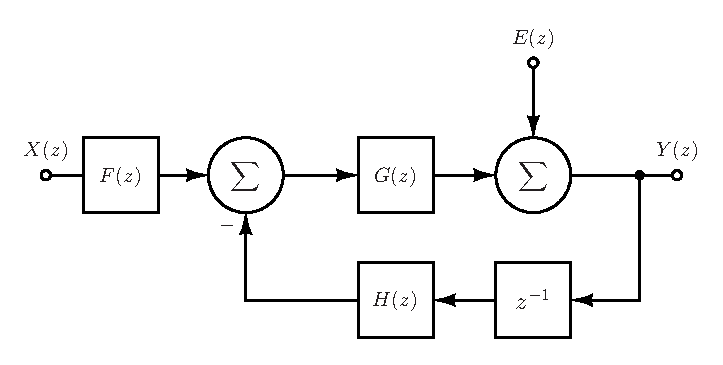
\includegraphics{./final_figures/linear_block_simulation.eps}
	\caption{$\Delta\Sigma$ Modulator Linear Model Block Diagram}
	\label{fig:linear_simulation_model_2}
\end{figure}
%-----------------------
As such, the NTF and STF represent discrete recursive filters, which are often designed
using digital IIR filter design techniques. The structure of a \DS modulator dictates
that the STF and NTF share a common set of poles. As such, the design of either the STF 
or NTF has implications for the design of the other. Because a \DS modulator's performance
depends mostly on the shape of the inband NTF, the NTF is typically designed first. The
zeros of the STF are then designed to accommodate the poles that result from the preceding
NTF design.

NTFs are often designed using traditional filters, such as Butterworth
and Chebyshev filters \cite{valkenburg_analog_1995}. These methods result in optimal
designs for certain performance criterion, often without consideration for others. For
example, a \DS modulator's NTF that has been designed using a Chebyshev filter is optimal
for dynamic range performance but not necessarily optimal for SNR performance.
Traditional filters such as Chebyshev filters generate NTFs with well defined passbands
which are not required for most NTFs. Also, these methods are not always easily adaptable
to the frequency response specifications required by \DS modulators for certain
applications \cite{IASTED_greg}.

Other contemporary methods often use numerical methods to determine optimal NTFs. For
example, the Delta Sigma Toolbox available for MATLAB\textsuperscript{\textregistered}
generates \DS modulator NTFs by determining NTF zeroes which minimize the
inband quantization noise power\cite{schreier_understanding_2004}. This technique
determines these optimized zeroes by setting the first derivative of the inband power
spectral density to zero and solving the resulting equations.  After determining the
optimized zeroes, the NTF's poles are optimized using an iterative approach. Because
poles and zeros do not affect system functions independently and because this
technique determines the NTF's zeros independently from its poles, this
technique does not necessarily generate optimal designs. As such, it will be shown that
this method offers only marginal improvement with respect to SNR over traditional
polynomial based methods.

In this thesis, the Hybrid Orthogonal Genetic (HOG) algorithm, developed in Chapter 3, is
used to determine optimal NTFs and STFs. The overall design methodology is illustrated in
Figure \ref{fig:HOG_DSM_flow}. Specifically, this implementation of the HOG algorithm
evolves optimal NTFs by maximizing a weighted combination of inband SNR and DR. After
determining an optimal NTF, the HOG algorithm then evolves an optimal STF by minimizing
 the passband magnitude error and attenuating out of band signal energy. The resulting
NTFs and STFs are then rigorously simulated and analyzed to ensure stability and
performance\cite{stubberud_hybrid_2008}.
%-----------------------
\begin{figure}[htbp]
	\centering
	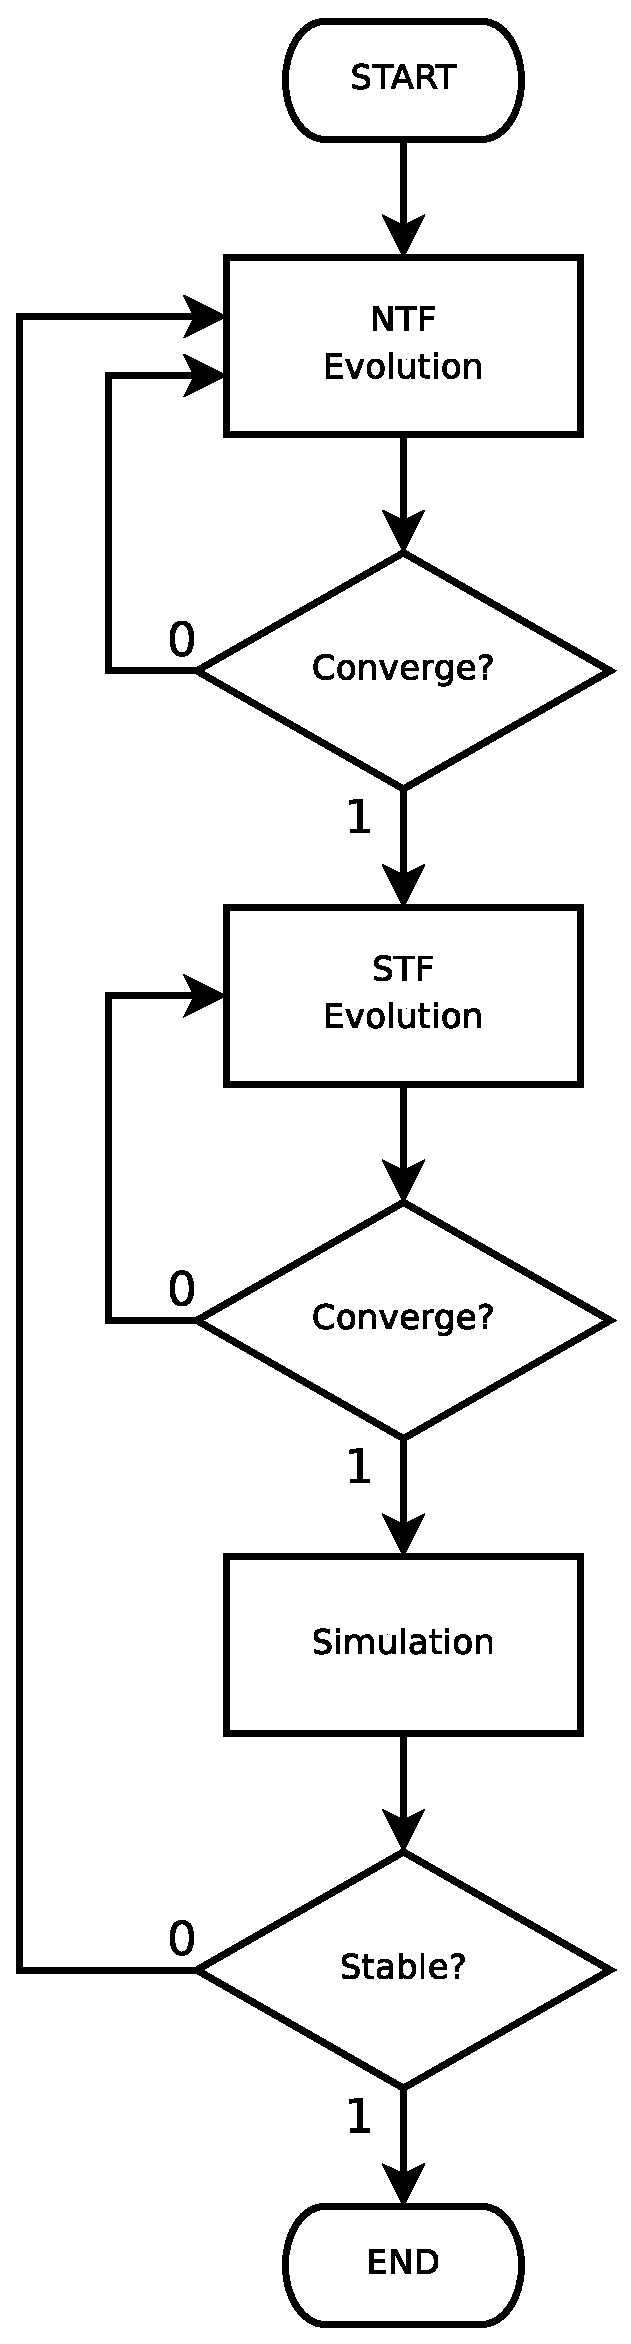
\includegraphics[height=0.65\textheight]{./final_figures/HOGA_DSM_flow.eps}
	\caption{Optimal \DS Modulator Design Flowchart}
	\label{fig:HOG_DSM_flow}
\end{figure}
%-----------------------

%%%%%%%%%%%%%%%%%%%%%%%%%%%%%%%%%%%%%%%%%%%%%%%%
% Section 4.2 - Objective Functions
%%%%%%%%%%%%%%%%%%%%%%%%%%%%%%%%%%%%%%%%%%%%%%%%
\section[Delta Sigma Modulator Design Objective Functions]
{$\Delta\Sigma$ Modulator Design Objective Functions}
\label{sec:DSM Design Objective Functions}
For this thesis, optimal NTFs and STFs are determined by approximating the NTF and STF
system functions so that the \DS modulator's SNR and DR are maximized. That is, cost
functions are minimized with respect to the NTF and STF coefficients such that the
effective resolution of the \DS modulator is maximized.

\subsection{NTF Objective Function}\label{sec:NTF_Objective_Function}
Ideally, a NTF magnitude response, $\lvert H(e^{j\omega})\rvert$,
would remove all signal energy in the stopband which implies that
%---------------------
\begin{equation}\label{eq:ideal_H_sb}
 \lvert H(e^{j\omega})\rvert=0,\qquad\omega\in\omega_\text{sb}
\end{equation}
%---------------------
where $\omega_\text{sb}$ is the set of stopband frequencies. For a lowpass \DS modulator,
$\omega_\text{sb}$, can be defined such that
$\omega_\text{sb}\in\{\omega:\lvert\omega\rvert\leq\omega_s\}$ for the stopband corner
frequency, $\omega_s$. However, to prevent the NTF from having all zero coefficients the
NTF's passband is ideally 1. Therefore, the ideal NTF magnitude response can be written as
%---------------------
\begin{equation}\label{eq:ideal_H_equation}
 \lvert H(e^{j\omega})\rvert=
\begin{cases}
0,& \omega\in\omega_\text{sb}\\
1,& \omega\in\omega_\text{pb}\\
\end{cases}
\end{equation}
%---------------------
where $\omega_\text{pb}$ is the set of passband frequencies. For a lowpass \DS modulator,
$\omega_\text{pb}$ can be defined such that
$\omega_\text{pb}\in\{\omega:\omega_p\leq\lvert\omega\rvert\leq\pi\}$ for the
passband corner frequency, $\omega_p$.
 
In practice, the ideal frequency response in \eqref{eq:ideal_H_equation} cannot be
achieved, and therefore, $\lvert H(e^{j\omega})\rvert$ must be approximated. As such, the
difference between the ideal magnitude response and the realized NTF magnitude response,
$\lvert\NTF(e^{j\omega})\rvert$, is referred to as the NTF magnitude response
error, $\lvert H_e(e^{j\omega})\rvert$; that is,
%---------------------
\begin{equation}\label{eq:H_error_mag}
 \lvert H_e(e^{j\omega})\rvert = \lvert
H(e^{j\omega})\rvert-\lvert\NTF(e^{j\omega})\rvert.
\end{equation}
%---------------------
Substituting \eqref{eq:ideal_H_equation} into \eqref{eq:H_error_mag}, it can be seen
that for a lowpass \DS modulator
%---------------------
\begin{equation}\label{eq:H_error_mag_2}
 \lvert H_e(e^{j\omega})\rvert=
\begin{cases}
\lvert \NTF(e^{j\omega})\rvert,& \omega\in\omega_\text{sb}\\
 1- \lvert\NTF(e^{j\omega})\rvert,& \omega\in\omega_\text{pb}
\end{cases}.
\end{equation}
%---------------------

\subsubsection{SNR Optimization}
To maximize the SNR over the NTF's stopband, the noise power in the NTF's stopband must be
minimized. As demonstrated by \eqref{eq:LTI_average_output_power} in Chapter \ref{ch:ADCs
and DSMs}, a \DS modulator's output quantization noise power, $P_q$, over the stopband can
be written as
%---------------------
\begin{equation}\label{eq:output_power_psd}
P_q=\frac{1}{2\pi}\int_{\omega\in\omega_\text{sb}}\lvert
\NTF(e^{j\omega})\rvert^2\bm{S}_e(e^{j\omega})d\omega
\end{equation}
%---------------------
where $\bm{S}_e(e^{j\omega})$ is the power spectral density of the quantization noise. As
shown in \eqref{eq:quantization_noise_psd_6},
$$\bm{S}_{e(n)}(e^{j\omega})=\frac{\Delta^2}{12}$$ which implies that
%---------------------
\begin{equation}\label{eq:output_noise_power}
P_q=\frac{\Delta^2}{12}\left(\frac{1}{2\pi}\right)\int_{\omega\in\omega_\text { sb } }
\lvert \NTF(e^{j\omega})\rvert^2 d\omega.
\end{equation}
%---------------------
Because the $p$-norm, denoted $\lVert\cdot\rVert_p$, of a continuous-time signal,
$x(t)$, is defined as
%---------------------
\begin{equation}\label{eq:p_norm}
\lVert x(t)\rVert_p=\left(\int_{t\in T}\lvert x(t)\rvert^p dt\right)^\frac{1}{p}
\end{equation}
%---------------------
where $T$ denotes some fixed time interval, $P_q$ can be written as
%---------------------
\begin{equation}\label{eq:parseval_3}
P_q=
\frac{\Delta^2}{12}\left(\frac{1}{2\pi}\right)\int_{\omega\in\omega_\text { sb } }
\lvert \NTF(e^{j\omega})\rvert^2 d\omega=
\frac{\Delta^2}{12}\left(\frac{1}{2\pi}\right)\lVert
\NTF(e^{j\omega})\rVert^2_{\twosub{2}{\omega\in\omega_\text{sb}}}.
\end{equation}
%---------------------
Therefore, a \DS modulator's SNR can be maximized by minimizing $\lVert
\NTF(e^{j\omega})\rVert^2_{\twosub{2}{\omega\in\omega_\text{sb}}}$.

\subsubsection{DR Optimization}
Recall that DR is defined as the ratio of the maximum to the minimum detectable
signal levels. As such, the DR can be maximized my minimizing the largest noise
component over the stopband of the NTF. Because the $\infty$-norm of a
continuous-time signal, $x(t)$, can be written as
%---------------------
\begin{equation}\label{eq:inf_norm}
\lVert x(t)\rVert_\infty=\lim_{p\to\infty}\left(\int_{t\in T}\lvert x(t)\rvert^p
dt\right)^\frac{1}{p}=\max\langle\lvert x(t)\rvert\rangle.
\end{equation}
%---------------------
Therefore, a \DS modulator's DR can be maximized by minimizing $\lVert
\NTF(e^{j\omega})\rVert_{\twosub{\infty}{\omega\in\omega_\text{sb}}}$.

\subsubsection{Passband Optimization}
It has been observed that the likelihood of \DS modulator stability can be increased by
designing NTFs that have approximately unity gain at $\pi$ radians/sample and that
 do not have passband peaking\cite{schreier_empirical_1993}. As such, minimizing the
1-norm of the magnitude error over the passband, $\lVert
1-\vert\NTF(e^{j\omega})\rvert\rVert_{\twosub{1}{\omega\in\omega_\text{pb}}}$, can
produce passband magnitude responses with approximately unity gain at $\pi$
radians/sample and that do not have passband peaking.

\subsubsection{Stability}
Because the NTF is modeled as discrete-time LTI systems, its pole locations,
$\left\{\gamma_k\right\}$, must lie within the unit circle to realize a stable system;
that is, for the \DS modulator to be stable, 
%---------------------
\begin{equation}\label{eq:stability}
\lvert \gamma_k \rvert < 1.
\end{equation}
%---------------------
As such, the solution space for the approximated NTF must be constrained such that none of
its poles lie outside the unit circle.

\subsubsection{Cost Function}
The NTF cost function is the weighted sum of the approximated magnitude response errors
and can be written as
%---------------------
\begin{equation}\label{eq:NTF_cost_function}
J_{\NTF}=
\alpha\lVert\NTF(e^{j\omega})\rVert^2_{\twosub{2}{\omega\in\omega_\text{sb}}}+
\beta\lVert\NTF(e^{j\omega})\rVert_{\twosub{\infty}{\omega\in\omega_\text{sb}}}+
\left(1-\alpha-\beta\right)\lVert 1-\lvert\NTF(e^{j\omega})\rvert\rVert_{\twosub{1}{
\omega\in\omega_\text{pb}}}
\end{equation}
%---------------------
where $\alpha$ and $\beta$ are weighting coefficients such that
$\left\{\alpha,\beta\right\}\geq0$ and $\alpha+\beta\leq1$, $\norm{\cdot}_p$ denotes the
$p$-norm, and all the pole locations are constrained such that they lie within the unit
circle.

As discussed in Chapter \ref{ch:ADCs and DSMs}, NTFs are typically modeled as LTI
systems that can be described by rational functions. Because minimizing the $p$-norm of a
rational function is a difficult analytical problem, the cost function is minimized
numerically. Thus, the NTF is approximated by calculating the DFT over the stopband and
the passband.

For example, the $N_s$-point DFT of the NTF can be written as
%---------------------
\begin{equation}\label{eq:sampling_frequency_response}
\NTF(k)=\NTF(e^{j\omega})\Bigr\rvert_{\omega=\frac{2\pi}{N_s}k}
\end{equation}
%---------------------
for $k\in\{I:0\leq k\leq N_s-1\}$. Thus,
%---------------------
\begin{equation}\label{eq:sampling_frequency_response_2}
\lVert\NTF(e^{j\omega})\rVert^2_{\twosub{2}{\omega\in\omega_\text{sb}}}
\approx
\quad\rVert\NTF(k)\rVert^2_{\twosub{2}{k\in k_\text{sb}}}
\end{equation}
%---------------------
where $k_\text{sb}\in\{k:0\leq k\leq N_s-1$ and
$\frac{2\pi}{N_s}k\in\omega_\text{sb}\}$ and where the $p$-norm of a discrete signal,
$x(n)$, is defined as
%---------------------
\begin{equation}\label{eq:vector_p_norm}
\lVert x(n)\rVert_p=\left(\sum_{k=1}^{N}\lvert x(k)\rvert^p\right)^\frac{1}{p}
\end{equation}
%---------------------
for a signal of length $N$. As such, the SNR can be maximized by minimizing the
2-norm squared of the approximated stopband frequency response,
$\lVert\NTF(k)\rVert^2_{\twosub{2}{k\in k_\text{sb}}}$, where
$k_\text{sb}=\left\{k:\frac{2\pi}{N_s}k\in\omega_\text{sb}\right\}.$ It can also be seen
that 
%---------------------
\begin{equation}\label{eq:vector_inf_norm_cont_equal}
\lVert\NTF(e^{j\omega})\rVert_{\twosub{\infty}{\omega\in\omega_\text{sb}}}
\approx
\quad\rVert\NTF(k)\rVert_{\twosub{\infty}{k\in k_\text{sb}}}
\end{equation}
%---------------------
where the $\infty$-norm of a discrete signal, $x(n)$, is defined as 
%---------------------
\begin{equation}\label{eq:vector_inf_norm}
\lVert x(n)\rVert_\infty=\lim_{p\to\infty}\left(\sum_{k=1}^{N}\lvert x(k)\rvert^p
\right)^\frac{1}{p}=\max\langle\lvert x(k)\rvert\rangle.
\end{equation}
%---------------------
for a signal of length $N$. As such, the DR can be maximized by minimizing the
$\infty$-norm of the approximated stopband frequency response,
$\lVert\NTF(k)\rVert_{\twosub{\infty}{k\in k_\text{sb}}}$, for
$$k_\text{sb}=\left\{k:\frac{2\pi}{N_s}k\in\omega_\text{sb}\right\}.$$

Similarly, the $N_p$-point DFT of the NTF can be written as 
%---------------------
\begin{equation}\label{eq:sampling_frequency_response_pb}
\NTF(k)=\NTF(e^{j\omega})\Bigr\rvert_{\omega=\frac{2\pi}{N_p}k}
\end{equation}
%---------------------
for $k\in\{I:0\leq k\leq N_p-1\}$. Thus,
%---------------------
\begin{equation}\label{eq:sampling_frequency_response_2_pb}
\lVert\NTF(e^{j\omega})\rVert_{\twosub{1}{\omega\in\omega_\text{pb}}}
\approx
\quad\rVert\NTF(k)\rVert_{\twosub{1}{k\in k_\text{pb}}}
\end{equation}
%---------------------
where $k_\text{pb}=\{k:0\leq k\leq N_p-1\text{ and
}\frac{2\pi}{N_p}k\in\omega_\text{pb}\}$. As such, the shape of the passband magnitude
response can be determined by minimizing the 1-norm of the approximated passband magnitude
error response, $\lVert1-\lvert\NTF(k)\rvert\rVert_{\twosub{1}{k\in k_\text{pb}}}$, for
$k_\text{pb}=\left\{k:\frac{2\pi}{N_p}k\in\omega_\text{pb}\right\}.$

Therefore, the NTF's objective function, $J_{\NTF}$, in \eqref{eq:NTF_cost_function} can
be approximated as 
%-----------------------
\begin{equation}\label{eq:NTF_objective_function}
J_{\NTF}=\\
\alpha\norm{\NTF(k)}^2_{\twosub{2}{k\in k_\text{sb}}}
+\beta\norm{\NTF(k)}_{\twosub{\infty}{k\in k_\text{sb}}}
+(1-\alpha-\beta)\norm{1-\lvert\NTF(k)\rvert}_{\twosub{1}{k\in k_\text{pb}}}
\end{equation}
%-----------------------
where $\left\{\alpha,\beta\right\}\geq0$ and $\alpha+\beta\leq1$ and all the pole
locations are constrained such that they lie within the unit circle. For this thesis,
optimal NTFs were designed with $\alpha=\beta=0.25$.

For example, the cost function illustrated in Figure \ref{fig:NTF_obj_fn} can be
minimized to determine a highpass NTF for a lowpass \DS modulator which is optimal
with respect to a weighted combination of SNR and DR.
%-----------------------
\begin{figure}[htbp]
	\centering
	\includegraphics*[clip,width=\textwidth,viewport=0 0 475
175]{./final_figures/NTF_objective_fn.eps}
	\caption{NTF Magnitude Response Objective Function}
	\label{fig:NTF_obj_fn}
\end{figure}
%-----------------------

\subsection{STF Objective Function}\label{sec:STF_Objective_Function}
Ideally, a STF magnitude response, $\lvert H(e^{j\omega})\rvert$,
would remove all signal energy in the stopband and the passband would be one; that is, an
ideal STF magnitude response, $\lvert H(e^{j\omega})\rvert$, can be written as
%---------------------
\begin{equation}\label{eq:ideal_H_equation_STF}
\lvert H(e^{j\omega})\rvert=
\begin{cases}
0,& \omega\in\omega_\text{sb}\\
1,& \omega\in\omega_\text{pb}\\
\end{cases}
\end{equation}
%---------------------
where $\omega_\text{sb}$ is the set of stopband frequencies and $\omega_\text{pb}$ is the
set of passband frequencies. In practice, the ideal frequency response in
\eqref{eq:ideal_H_equation_STF} cannot be achieved, and therefore, $\lvert
H(e^{j\omega})\rvert$ must be approximated. As such, the difference between the ideal
magnitude response and the realized STF magnitude response, $\lvert
\STF(e^{j\omega})\rvert$, is referred to as the STF magnitude response
error, $H_e(e^{j\omega})$; that is,
%---------------------
\begin{equation}\label{eq:H_error_mag_STF}
 H_e(e^{j\omega})= \lvert H(e^{j\omega})\rvert-\lvert\STF(e^{j\omega})\rvert.
\end{equation}
%---------------------
Comparing \eqref{eq:ideal_H_equation_STF} and \eqref{eq:H_error_mag_STF}, it can be seen
that for a lowpass \DS modulator
%---------------------
\begin{equation}\label{eq:H_error_mag_2_STF}
\lvert H_e(e^{j\omega})\rvert=
\begin{cases}
\lvert \STF(e^{j\omega})\rvert,& \omega\in\omega_\text{sb}\\
 1- \lvert\STF(e^{j\omega})\rvert,& \omega\in\omega_\text{pb}
\end{cases}
\end{equation}
%---------------------

\subsubsection{STF Optimization}
Recall that the stopband signal energy can be minimized by minimizing the 2-norm squared
of the frequency response, $\lVert \STF(e^{j\omega})\rVert^2_2$, for $\omega
\in\omega_\text{sb}$. Similarly, minimizing the 1-norm of the passband magnitude error,
$\lVert 1- \lvert\STF(e^{j\omega})\rvert\rVert_1$, for $\omega\in\omega_\text{pb}$
produces magnitude responses which are approximately unity gain and without
passband peaking.

\subsubsection{Cost Function}
Therefore, the STF cost function, which is the weighted sum of the
approximated magnitude response errors, can be written as
%---------------------
\begin{equation}\label{eq:STF_cost_function}
J_{\STF}=
\zeta\lVert\STF(e^{j\omega})\rVert^2_{\twosub{2}{\omega\in\omega_\text{sb}}}+
\left(1-\zeta\right)\lVert 1-\lvert\STF(e^{j\omega})\rvert\rVert_{\twosub{1}{
\omega\in\omega_\text{pb}}}
\end{equation}
%---------------------
where $\zeta$ is a weighting coefficients such that $0\leq\zeta\leq1$ and $\norm{\cdot}_p$
denotes the $p$-norm.

However, as discussed in Chapter \ref{ch:ADCs and DSMs}, STFs are typically modeled as LTI
systems that can be described by rational functions. Because minimizing the $p$-norm of a
rational function is a difficult analytical problem, the cost function is minimized
numerically. Thus, the STF is approximated by calculating the DFT over the stopband and
the passband.

As was done for the NTF, an $N_s$-point DFT and a $N_p$-point DFT can be used to
approximate the cost function given in \eqref{eq:STF_cost_function} such that 
%-----------------------
\begin{equation}\label{eq:STF_objective_function}
J_{\STF}=
\zeta\norm{\STF(k)}^2_{\twosub{2}{k\in k_\text{sb}}}
+(1-\zeta)\norm{1-\lvert\STF(k)\rvert}_{\twosub{1}{k\in k_\text{pb}}}
\end{equation}
%-----------------------
where $0\leq\zeta\leq1$. For this thesis, optimal STFs were designed with a weighting
coefficient of $\zeta=0.5$.

For example, the cost function illustrated in Figure \ref{fig:STF_obj_fn} can be
minimized to determine an optimal STF for a lowpass \DS modulator.
%-----------------------
\begin{figure}[htbp]
	\centering
	\includegraphics*[clip,width=\textwidth,viewport=0 0 475
175]{./final_figures/STF_objective_fn.eps}
	\caption{STF Magnitude Response Objective Function}
	\label{fig:STF_obj_fn}
\end{figure}
%-----------------------

\subsection{Objective Function Minimization}
The cost functions shown in \eqref{eq:NTF_objective_function} and
\eqref{eq:STF_objective_function} are known to be highly multimodal and non-differentiable
equations\cite{rabiner_linear_1974}. As such, the HOG algorithm presented in Chapter
\ref{ch:Optimization and Genetic Algorithms} has been implemented as a constrained global
optimizer to minimize the cost functions thereby producing \DS modulator system functions
which are optimal with respect to their cost functions.

The HOG algorithm constrains the solution space through penalization. For example, a large
penalty value is returned if any of the evolved poles fall outside the unit circle. In
addition, the general shape of the magnitude response is constrained such that proposed
filter solutions which do not conform to the desired magnitude response shape (e.g.
highpass or lowpass) are penalized. For example, the NTF magnitude response evaluated at
DC must be sufficiently low or a large penalty value is returned. Similarly, the STF
magnitude response evaluated at $\pi$ radians/sample must be sufficiently low or a large
penalty value is returned. In general, penalties are selected so that they do  not
restrict the solution space any more than necessary which has been shown to result in
sub-optimal solutions \cite{karaboga_design_2004}.

%%%%%%%%%%%%%%%%%%%%%%%%%%%%%%%%%%%%%%%%%%%%%%%%
% Section 4.2 - HOG Algorithm Implementation
%%%%%%%%%%%%%%%%%%%%%%%%%%%%%%%%%%%%%%%%%%%%%%%%
\section{HOG Algorithm Implementation}\label{sec:HOG Algorithm Implementation}
For this thesis, the HOG algorithm, developed in Chapter \ref{ch:Optimization and Genetic
Algorithms}, is used to evolve a population
of chromosomes which contain the polynomial coefficients for the rational functions which
represent the NTF and STF. Once the population has been initialized to the regions
surrounding the solutions of traditional polynomials (e.g the Chebyshev polynomial), the
HOG algorithm iteratively evolves better polynomial coefficients until the population
converges to the optimum. For this implementation, the optimal polynomial coefficients are
determined by minimizing the cost functions in \eqref{eq:NTF_objective_function} and
\eqref{eq:STF_objective_function} thereby producing system functions which are optimal
with respect to SNR and DR.

%%%%%%%%%%%%%%%%%%%%%%%%%%%%%%%%%%%%%%%%%%%%%%%%
% Section 4.2.2 - Chromosome and Population Structure
%%%%%%%%%%%%%%%%%%%%%%%%%%%%%%%%%%%%%%%%%%%%%%%%
\subsection{Chromosome and Population Structure}\label{sec:Chromosome and Population
Structure}
Recall that structurally, chromosomes are implemented as arrays of length $K$. As such,
these arrays are populated with $K$ alleles, that are iteratively modified
during the evolutionary process. For filter design applications, the alleles can
correspond to the polynomial coefficients of the NTF or STF which have the general form
%---------------------
\begin{equation}\label{eq:chromosome_NTF_polynomial}
H(z)=\frac{\displaystyle\sum_{n=0}^{N}{a_n
z^{-n}}}{\displaystyle\sum_{n=0}^{N}{b_n z^{-n}}}
\end{equation}
%---------------------
where $\{a_{n}\}$ and $\{b_{n}\}$ are the sets of real polynomial coefficients and $N$ is
the order of the filter. However, populating the chromosomes directly with the polynomial
coefficients,
$\{a_n\}$ and $\{b_n\}$, yields chromosomes which are very sensitive to perturbation
during the evolutionary process. To reduce coefficient sensitivity,
\eqref{eq:chromosome_NTF_polynomial} can be written in its zero-pole-gain form,
%---------------------
\begin{equation}\label{eq:chromosome_NTF_pole_zero}
H(z)=\psi\cdot\frac{\displaystyle\prod_{n=1}^{N}{\bigl(1-c_n z^{-1}\bigr)}}
{\displaystyle\prod_{n=1}^{N}{\bigl(1-d_n z^{-1}\bigr)}}
\end{equation}
%---------------------
where $\{c_n\}$ is the set containing the system function's zeros, $\{d_n\}$ is the set
containing the system function's poles, and $\psi$ represents the system function's gain.
The alleles then correspond to the system function's zeros, poles, and gain. However, for
filters with real coefficients, these algorithms must explicitly manage complex conjugate
pairs of poles and zeros which can significantly lengthen run times. To reduce coefficient
sensitivity and simplify the management of complex conjugate pairs of poles and zeros, the
chromosomes are structured specifically so that the system function, $H(z)$, has the form
%---------------------
\begin{equation}\label{eq:chromosome_NTF}
H(z)=\psi\biggl(\frac{1-a_1 z^{-1}}{1-b_1 z^{-1}}\biggr)^m
\displaystyle\prod_{n=1}^{M}\frac{\bigl(1+c_{1n}z^{-1}+c_{2n}z^{-2}\bigr)}{\bigl(1+d_{1n}
z^{-1}+d_{2n}z^{-2}\bigr)}
\end{equation}
%---------------------
where $M$ is the number of second-order-sections, $\psi$ represents the system
function's gain, and $m$ is 1 or 0 for odd or even ordered systems,
respectively\cite{kit-sang_tang_design_1998}.
 
For this thesis, the NTF is equivalent to \eqref{eq:chromosome_NTF}; that
is
%---------------------
\begin{equation}\label{eq:NTF_system_function}
\NTF(z)=\psi_N\biggl(\frac{1-a_1 z^{-1}}{1-b_1 z^{-1}}\biggr)^m
\displaystyle\prod_{n=1}^{M}\frac{\bigl(1+c_{1n}z^{-1}+c_{2n}z^{-2}\bigr)}{\bigl(1+d_{1n}
z^{-1}+d_{2n}z^{-2}\bigr)}\text{.}
\end{equation}
%---------------------
Thus, for a NTF described by \eqref{eq:NTF_system_function},
the structural chromosome array, $\mathcal{C}_{\text{NTF}}$, of length, $K_N$, where
%---------------------
\begin{equation}\label{eq:NTF_chromosome_length}
 K_N=4M+2m+1,
\end{equation}
%---------------------
can be written as
%---------------------
\begin{equation}\label{eq:chromosome_array_even}
\mathcal{C}_{\text{NTF}}=\left[c_{11},c_{12},d_{11},d_{12},c_{21},c_{22},d_{21},d_{
22},\dotsc,c_{M1},c_{M2},d_{M1},d_{M2},\psi_N\right]^T
\end{equation}
%---------------------
for even ordered systems and
%---------------------
\begin{equation}\label{eq:chrmosome_array_odd}
\mathcal{C}_{\text{NTF}} =
\left[a_1,b_1,c_{11},c_{12},d_{11},d_{12},c_{21},c_{22},d_{ 21},
d_{22},\dotsc,c_{M1},c_{M2},d_{M1},d_{M2},\psi_N\right]^T
\end{equation}
%---------------------
for odd ordered systems where the superscript $T$ denotes the transpose operator. As such,
for a NTF of order $2M+1$, a population, $\mathbb{G}_{\text{NTF}}$, of $n$ chromosomes can
be written as
%---------------------
\begin{equation}\label{eq:population}
\mathbb{G}_{\text{NTF}}
=\Bigl[\mathcal{C}_{\text{NTF},1}\dashline\mathcal{C}_{\text{NTF},2}
\dashline\dotsb\dashline\mathcal{C}_{\text{NTF},n}\Bigr]=
\begin{pmatrix}
a_{1,1}&  a_{1,2}& \hdotsfor{1}& a_{1,n-1}& a_{1,n} \\
b_{1,1}&  b_{1,2}& \hdotsfor{1}& b_{1,n-1}& b_{1,n} \\
c_{11,1}&  c_{11,2}& \hdotsfor{1}& c_{11,n-1}& c_{11,n} \\
c_{12,1}&  c_{12,2}& \hdotsfor{1}& c_{12,n-1}& c_{12,n} \\
d_{11,1}&  d_{11,2}& \hdotsfor{1}& d_{11,n-1}& d_{11,n} \\
d_{12,1}& d_{12,2}& \hdotsfor{1}& d_{12,n-1}& d_{12,n} \\
\vdots&\vdots&\ddots&\vdots&\vdots\\
c_{M1,1}& c_{M1,2}&\hdotsfor{1}& c_{M1,n-1}& c_{M1,n} \\
c_{M2,1}& c_{M2,2}&\hdotsfor{1}& c_{M2,n-1}& c_{M2,n} \\
d_{M1,1}& d_{M1,2}&\hdotsfor{1}& d_{M1,n-1}& d_{M1,n} \\
d_{M2,1}& d_{M2,2}&\hdotsfor{1}& d_{M2,n-1}& d_{M2,n} \\
\psi_{N,1}& \psi_{N,2}&\hdotsfor{1}& \psi_{N,n-1}& \psi_{N,n} \\	
\end{pmatrix}
\end{equation}
%-----------------------
where $\mathbb{G}_{\text{NTF}}$ is a $K_N\times n$ matrix and $\mathcal{C}_{\text{NTF},n}$
is the $n$th chromosome. 

Because NTFs and STFs share a common set of poles and the NTF is designed first, the STF
system function can be written as
%---------------------
\begin{equation}\label{eq:STF_system_function}
 \STF(z)=\psi_S\biggl(\frac{1-\rho_1 z^{-1}}{1-b_1 z^{-1}}\biggr)^m
\displaystyle\prod_{n=1}^{M}\frac{\bigl(1+\nu_{1n}z^{-1}+\nu_{2n}z^{-2}\bigr)}{\bigl(1+d_{
1n }z^{-1}+d_{2n}z^{-2}\bigr)}\text{.}
\end{equation}
%---------------------
Because the pole locations are established by the design of the NTF, only the STF's zero
locations are perturbated during the optimization process. As such, for a STF system
function described by \eqref{eq:STF_system_function},
the structural chromosome array, $\mathcal{C}_{\text{STF}}$, of length $K_S$, where
%---------------------
\begin{equation}\label{eq:STF_chromosome_length}
 K_S=2M+m+1,
\end{equation}
%---------------------
can be written as
%---------------------
\begin{equation}\label{eq:STF_chromosome_array_even}
\mathcal{C}_{\text{STF}}=\left[\nu_{11},\nu_{12},\nu_{21},\nu_{22},\dotsc,\nu_{M1},
\nu_{M2},\psi_S\right]^T
\end{equation}
%---------------------
for even ordered systems and
%---------------------
\begin{equation}\label{eq:STF_chrmosome_array_odd}
\mathcal{C}_{\text{STF}} =
\left[\rho_1,\nu_{11},\nu_{12},\nu_{21},\nu_{22},\dotsc,\nu_{M1},\nu_{M2},
\psi_S\right]^T
\end{equation}
%---------------------
for odd ordered systems. As such, for a STF of order $2M+1$, a population,
$\mathbb{G}_{\text{STF}}$, of $n$ chromosomes can be written as
%---------------------
\begin{equation}\label{eq:STF_population}
\mathbb{G}_{\text{STF}}
=\Bigl[\mathcal{C}_{\text{STF},1}\dashline\mathcal{C}_{\text{STF},2}
\dashline\dotsb\dashline\mathcal{C}_{\text{STF},n}\Bigr]=
\begin{pmatrix}
\rho_{1,1}&  \rho_{1,2}& \hdotsfor{1}& \rho_{1,n-1}& \rho_{1,n} \\
\nu_{11,1}&  \nu_{11,2}& \hdotsfor{1}& \nu_{11,n-1}& \nu_{11,n} \\
\nu_{12,1}&  \nu_{12,2}& \hdotsfor{1}& \nu_{12,n-1}& \nu_{12,n} \\
\vdots&\vdots&\ddots&\vdots&\vdots\\
\nu_{M1,1}& \nu_{M1,2}&\hdotsfor{1}& \nu_{M1,n-1}& \nu_{M1,n} \\
\nu_{M2,1}& \nu_{M2,2}&\hdotsfor{1}& \nu_{M2,n-1}& \nu_{M2,n} \\
\psi_{S,1}& \psi_{S,2}&\hdotsfor{1}& \psi_{S,n-1}& \psi_{S,n} \\	
\end{pmatrix}
\end{equation}
%-----------------------
where $\mathbb{G}_{\text{STF}}$ is a $K_S\times n$ matrix and
$\mathcal{C}_{\text{STF},n}$ is the $n$th chromosome. 

%%%%%%%%%%%%%%%%%%%%%%%%%%%%%%%%%%%%%%%%%%%%%%%%
% Section 4.2.3 - Algorithm Parameters
%%%%%%%%%%%%%%%%%%%%%%%%%%%%%%%%%%%%%%%%%%%%%%%%
\subsection{Algorithm Parameters}\label{sec:Algorithm Paramters}
The relative size of a population dictates the nature of the results. For example, large
unconstrained populations offer a broad evaluation of the performance surface at the
expense of convergence speed and steady-state misadjustment. Conversely, small
constrained populations converge quickly at the expense of increased population
variance. Further, selecting the appropriate size for a population is directly related
to the complexity, or dimensionality, of the problem space. However, the relationship
between problem space complexity and requisite population size is typically either poorly
defined or unknown \cite{alander_optimal_1992}. As such, for constrained problem spaces,
the most important concept is often minimum population size. However, because the minimum
population size is tightly coupled with the problem space complexity and therefore poorly
defined, it is typically refined or tuned a
posteriori\cite{alander_optimal_1992}\cite{schaffer_-_1989}. 

For this thesis, the initial size of the population has been restricted to 200; that is, 
to determine optimal NTFs and STFs, the HOG algorithm was initially configured with a
population size of 200 chromosomes. Because the poles of an IIR filter must
lie within the unit circle for the filter to be stable, the feasible solutions space
has been constrained such that each pole location, $\gamma$, lies within the unit circle
which implies that $$\lvert\gamma\rvert\leq1\text{.}$$ Because the interaction between
transfer function poles and zeros is implied in the desired magnitude response,
constraining the pole locations also indirectly constrains the zero locations. The
remaining HOG algorithm parameters are summarized in Table \ref{tbl:hog_dsm_setup}.
%----------------------------
\begin{table}[htbp]
 \begin{center}
 \caption[LP$\Delta\Sigma$M HOG Algorithm Parameters]{Low-Pass $\Delta\Sigma$ Modulator
Design: HOG Algorithm Parameters}
 \label{tbl:hog_dsm_setup}
 \begin{tabular}{ l c }\toprule
 \textbf{Description} & \textbf{Value} \\ \midrule
Problem Dimension & $K: K=K_N \text{or} K_S$ \\
Population Size & $200$ \\
Feasible Solution Space & $\lvert\gamma\rvert\leq1$ \\
Probability of Crossover & $P_c = 0.2$ \\
Probability of Mutation & $P_m = 0.02$ \\
Selection Pressure & $\eta^+ = 1.1$\\ \bottomrule
\end{tabular}
\end{center}
\end{table}

%%%%%%%%%%%%%%%%%%%%%%%%%%%%%%%%%%%%%%%%%%%%%%%%
% Section 4.2.4 - Population Initialization
%%%%%%%%%%%%%%%%%%%%%%%%%%%%%%%%%%%%%%%%%%%%%%%%
\subsection{Population Initialization}\label{sec:Population Initialization}
Although global optimization algorithms do not require a priori knowledge of
the performance surface to determine the optimum solution,  generalized constraints on
the objective function's solution space can greatly increase the speed of the algorithm's
convergence. Seeding the population with known solutions is often employed as a
test for conversion latency\cite{sarker_evolutionary_2002}. It has also been shown  that
seeding the population with solutions which are known to be near optimal can lead
to optimal solutions\cite{sarker_evolutionary_2002}.

Discrete-time \DS modulator NTFs which are designed using both contemporary and
traditional techniques have zeros which are distributed on or near segments of the unit
circle which correspond with the NTF's
stopband\cite{valkenburg_analog_1995}\cite{schreier_understanding_2004}.
Thus, it is plausible that the optimal zero locations will be distributed on or near
segments of the unit circle which correspond with the NTF's stopband as well. Further, if
it is assumed that the optimal zero locations are
distributed on or near the unit circle, then the optimal pole locations will likely be
proximal to the pole locations of both the traditional and contemporary NTF
filter designs.

Similarly, discrete-time \DS modulator STFs which are designed using traditional
techniques have zeroes which are distributed on or near the segments of the unit circle
corresponding to the STF's stopband. Thus, it is plausible that the optimal
zero locations will be distributed on or near segments of the unit circle which
correspond to the STF's stopband, as well. However, unlike the
NTF, which is designed first, the pole locations of the STF are fixed by the NTF design.
As such, it is assumed that the zero locations will be proximal to the zero locations for
traditional STF filter designs with pole locations determined by the optimal design of
the NTF.

Thus, the initial NTF and STF populations, $\mathbb{G}_{\NTF,0}$ and
$\mathbb{G}_{\STF,0}$, are seeded with chromosomes whose alleles are selected randomly
about the coefficients of a comparable NTF or STF, respectively. Specifically, their
respective chromosomes are determined by adding zero mean, standard normal random dither,
represented by $x$, with a fixed variance of 10\% (normalized with respect to the unit
circle) to the each of the Chebyshev polynomial coefficients where the system function is
described by \eqref{eq:chromosome_NTF} or \eqref{eq:STF_system_function}; that is, the
$k$th additive dither element, $\delta_k$, where $\bigl\{k\in I:1\leq k\leq
\left(K_N \;\text{or}\; K_S\right)\bigr\}$, can be expressed as 
%---------------------
\begin{equation}\label{eq:init_dither}
\delta_{k}=\frac{1}{\sqrt{0.2\pi}}e^{-\frac{x^2}{0.2}}
\end{equation}
%---------------------
for the random variable $x$.
 
Thus, the $n$th dithered chromosome,
$\tilde{\mathcal{C}}_{\NTF,n}$, belonging to an initial NTF population,
$\mathbb{G}_{\NTF,0}$, with a system function of order $2M+1$, can be written as 
%---------------------
\begin{equation}\label{eq:dithered_chromosome}
\begin{split}
&\tilde{\mathcal{C}}_{\NTF,n}= \\
&\bigl[
(a_{1}+\delta_{N,1}),(b_{1}+\delta_{N,2}),(c_{11}+\delta_{N,3}),(c_{12}+\delta_{N,4}),(d_
{ 11 }
+\delta_{N,5}),(d_{12}+\delta_{N,6}),\dotsc \\
&(c_{M1}+\delta_{N,K_N-4}),(c_{M2}+\delta_{N,K_N-3}),(d_{M1}+\delta_{N,K_N-2}),(d_{
M2 }
+\delta_{N,K_N-1}),(\psi_N+\delta_{N,K_N})\bigr]^T\\
&=\bigl[
\tilde{a}_1,\tilde{b}_1,\tilde{c}_{11},\tilde{c}_{12},\tilde{d}_{11},\tilde{d}_{12},
\tilde { c } _ { 21 } ,
\tilde{c}_{22},
\tilde{d}_{21},\tilde{d}_{22},\dotsc,\tilde{c}_{M1},\tilde{c}_{M2},\tilde{d}_{M1},
\tilde{d}_{M2},\tilde{\psi}_N\bigr]^T.
\end{split}
\end{equation}
%---------------------
where $\delta_{N,k}$ corresponds to the $k$th NTF additive dither element. Because a
population is defined as the aggregate of $n$ chromosomes, the initial
NTF population, $\mathbb{G}_{\NTF,0}$, can be written as
%---------------------
\begin{equation}
\mathbb{G}_{\NTF,0}
=\bigl[\tilde{\mathcal{C}}_{\NTF,1}\dashline\tilde{\mathcal{C}}_{\NTF,2}\dashline
\dotsb\dashline\tilde{\mathcal{C}}_{\NTF,n}\bigr]=
\begin{pmatrix}
\tilde{a}_{11,1}&\tilde{a}_{11,2}&\hdotsfor{1}&\tilde{a}_{11,n-1}&\tilde{a}_{11,n} \\
\tilde{b}_{12,1}&\tilde{b}_{12,2}&\hdotsfor{1}&\tilde{b}_{12,n-1}&\tilde{b}_{12,n} \\
\tilde{c}_{11,1}&\tilde{c}_{11,2}&\hdotsfor{1}&\tilde{c}_{11,n-1}&\tilde{c}_{11,n} \\
\tilde{c}_{12,1}&\tilde{c}_{12,2}&\hdotsfor{1}&\tilde{c}_{12,n-1}&\tilde{c}_{12,n} \\
\tilde{d}_{11,1}&\tilde{d}_{11,2}&\hdotsfor{1}&\tilde{d}_{11,n-1}&\tilde{d}_{11,n} \\
\tilde{d}_{12,1}&\tilde{d}_{12,2}&\hdotsfor{1}&\tilde{d}_{12,n-1}&\tilde{d}_{12,n} \\
\vdots&\vdots&\ddots&\vdots&\vdots						   \\
\tilde{c}_{M1,1}&\tilde{c}_{M1,2}&\hdotsfor{1}&\tilde{c}_{M1,n-1}&\tilde{c}_{M1,n} \\
\tilde{c}_{M2,1}&\tilde{c}_{M2,2}&\hdotsfor{1}&\tilde{c}_{M2,n-1}&\tilde{c}_{M2,n} \\
\tilde{d}_{M1,1}&\tilde{d}_{M1,2}&\hdotsfor{1}&\tilde{d}_{M1,n-1}&\tilde{d}_{M1,n} \\
\tilde{d}_{M2,1}&\tilde{d}_{M2,2}&\hdotsfor{1}&\tilde{d}_{M2,n-1}&\tilde{d}_{M2,n} \\
\tilde{\psi}_{N,1}&\tilde{\psi}_{N,2}&\hdotsfor{1}&\tilde{\psi}_{N,n-1}&\tilde{\psi}_{N,n
} \\
\end{pmatrix}
\end{equation}
where $\mathbb{G}_{\NTF,0}$ is a $K_N\times n$ matrix and $\tilde{\mathcal{C}}_{\NTF,k}$
is the $k$th dithered chromosome.

Similarly, the $n$th dithered chromosome, $\tilde{\mathcal{C}}_{\STF,n}$, belonging to an
initial STF population, $\mathbb{G}_{\STF,0}$, with a system function of order $2M+1$ can
be written as 
%---------------------
\begin{equation}\label{eq:dithered_chromosome_STF}
\begin{split}
\tilde{\mathcal{C}}_{\STF,n}=\bigl[
(\rho_{1}+\delta_{S,1}),(\nu_{11}+\delta_{S,2}),(\nu_{12}+\delta_{S,3}),\dotsc\\
 \dotsc,(\nu_{M1}+\delta_ { S,K_S-2 } ) ,
(\nu_{M2}+\delta_{S,K_S-1}),(\psi_S+\delta_{S,K_S})\bigr]^T\\
=\bigl[
\tilde{\rho_1},\tilde{\nu}_{11},\tilde{\nu}_{12},\tilde{\nu}_{21},\tilde{\nu}_{22},\dotsc,
\tilde{\nu}_{M1},\tilde{\nu}_{M2},\tilde{\psi}_S\bigr]^T
\end{split}
\end{equation}
%---------------------
where $\delta_{S,k}$ corresponds to the $k$th STF additive dither element. Because a
population is defined as the aggregate of $n$ chromosomes, the initial
STF population, $\mathbb{G}_{\STF,0}$, can be written as
%---------------------
\begin{equation}
\mathbb{G}_{\STF,0}
=\bigl[\tilde{\mathcal{C}}_{\STF,1}\dashline\tilde{\mathcal{C}}_{\STF,2}\dashline
\dotsb\dashline\tilde{\mathcal{C}}_{\STF,n}\bigr]=
\begin{pmatrix}
\tilde{\rho}_{11,1}&\tilde{\rho}_{11,2}&\hdotsfor{1}&\tilde{\rho}_{11,n-1}&\tilde{\rho}_{
11,n } \\
\tilde{\nu}_{11,1}&\tilde{\nu}_{11,2}&\hdotsfor{1}&\tilde{\nu}_{11,n-1}&\tilde{\nu}_{11,n}
\\
\tilde{\nu}_{12,1}&\tilde{\nu}_{12,2}&\hdotsfor{1}&\tilde{\nu}_{12,n-1}&\tilde{\nu}_{12,n}
\\
\vdots&\vdots&\ddots&\vdots&\vdots						   \\
\tilde{\nu}_{M1,1}&\tilde{\nu}_{M1,2}&\hdotsfor{1}&\tilde{\nu}_{M1,n-1}&\tilde{\nu}_{M1,n}
\\
\tilde{\nu}_{M2,1}&\tilde{\nu}_{M2,2}&\hdotsfor{1}&\tilde{\nu}_{M2,n-1}&\tilde{\nu}_{M2,n}
\\
\tilde{\psi}_{S,1}&\tilde{\psi}_{S,2}&\hdotsfor{1}&\tilde{\psi}_{S,n-1}&\tilde{\psi}_{S,n
} \\	
\end{pmatrix}
\end{equation}
where $\mathbb{G}_{\STF,0}$ is a $K_S\times n$ matrix and $\tilde{\mathcal{C}}_{\STF,k}$
is the $k$th dithered chromosome. 

%%%%%%%%%%%%%%%%%%%%%%%%%%%%%%%%%%%%%%%%%%%%%%%%
% Section 4.2.5 - Convergence
%%%%%%%%%%%%%%%%%%%%%%%%%%%%%%%%%%%%%%%%%%%%%%%%
\subsection{Convergence}\label{sec:Convergence}
Convergence during the evolution of a particular NTF or STF is defined as the lack of
further improvement over 100 successive generations following a minimum of 1000
generations. This criterion improves the probability that the evolved transfer functions
will be optimal with respect to their objective functions. However, this optimality does
not guarantee overall system stability; that is, even optimized NTFs and STFs may be
unstable when implemented in a $\Delta\Sigma$ modulator. Thus, overall design convergence
is achieved when the \DS modulator is stable and the observed DR and SNR are better than
the observations made for both traditional and contemporary $\Delta\Sigma$ modulator
designs of like order and OSR.

%%%%%%%%%%%%%%%%%%%%%%%%%%%%%%%%%%%%%%%%%%%%%%%%
% Section 4.3 - Simulation and Modeling
%%%%%%%%%%%%%%%%%%%%%%%%%%%%%%%%%%%%%%%%%%%%%%%%
\section{Simulation and Modeling}\label{sec:Simulation and Modeling}
Because SNR and DR are measures of an ADC's effective resolution and because SNR and DR
are measured in the frequency domain, the performance of a \DS modulator is characterized
by its observed output spectrum. While the linear quantizer model shown in Figure
\ref{fig:linear_quantizer_model} is sufficient for theoretical results and preliminary
system modeling, a simulation of the nonlinear system is necessary to determine the
realized effective resolution of a \DS modulator \cite{schreier_empirical_1993}. Thus, the
designed systems were verified using a simulator based on the block diagram shown in
Figure \ref{fig:linear_simulation_model_2}.

For this thesis, the output, $y(n)$, of a discrete-time \DS modulator is determined
using the linear difference equations which correspond to the blocks shown
in Figure \ref{fig:linear_simulation_model_2}. The \DS modulator's output is then
bandlimited to the Nyquist frequency of the input signal, $f_{\text{NQ}}$, where
$f_{\text{NQ}}\in\left[-f_s/2\text{OSR},f_s/2\text{OSR}\right]$, and then decimated by a
factor of $\text{OSR}/2$. Finally, the SNR and DR are calculated
using frequency domain analysis of the spectrum of the decimated output signal.

%%%%%%%%%%%%%%%%%%%%%%%%%%%%%%%%%%%%%%%%%%%%%%%%
% Section 4.3.1 - Linear Difference Equations
%%%%%%%%%%%%%%%%%%%%%%%%%%%%%%%%%%%%%%%%%%%%%%%%
\subsection{Linear Difference Equations}\label{sec:Linear Difference Equations}
Recall that the output, $y(n)$, of a \DS modulator as shown in Figure
\ref{fig:linear_simulation_model_2} can be expressed as 
%-----------------------
\begin{equation}\label{eq:general_form}
 Y(z) =\STF(z)X(z)+\NTF(z)E(z)
 \end{equation}
%-----------------------
where
%-----------------------
\begin{equation}\label{eq:STF_solution_1}
\STF(z)=\frac{F(z)G(z)}{1+z^{-1}G(z)H(z)}
\end{equation}
%-----------------------
and
%-----------------------
\begin{equation}\label{eq:NTF_solution_1}
\NTF(z)=\frac{1}{1+z^{-1}G(z)H(z)}\text{.}
\end{equation}
%-----------------------
Because STFs and NTFs are modeled as linear recursive filters, they can be written as
%-----------------------
\begin{equation}\label{eq:STF_poly_form}
\text{STF}(z)=\frac
{\displaystyle\sum_{k=0}^{N}{\alpha_k z^{-k}}}
{\displaystyle\sum_{k=0}^{N}{\beta_k  z^{-k}}}
\end{equation}
%-----------------------
and
%-----------------------
\begin{equation}\label{eq:NTF_poly_form}
\text{NTF}(z)=\frac
{\displaystyle\sum_{k=0}^{N}{\gamma_k z^{-k}}}
{\displaystyle\sum_{k=0}^{N}{\beta_k  z^{-k}}}
\end{equation}
%-----------------------
where $\{\alpha_k\}$, $\{\beta_k\}$, and $\{\gamma_k\}$ are the sets of real coefficients,
$\beta_0=1$, and
$N$ is the order of the numerator and denominator polynomials. 

\subsubsection{Canonical Solution}\label{sec:Canonical Solution}
Because $F(z)$, $G(z)$, and $H(z)$ are rational functions,
the STF and NTF can be expressed as
%-----------------------
\begin{equation}\label{eq:block_diagram_solving_STF}
\text{STF}(z) =\frac
{\left(\displaystyle\frac{F_n(z)}{F_d(z)}\displaystyle\frac{G_n(z)}{G_d(z)}\right)}
{1+z^{-1}\left(\displaystyle\frac{G_n(z)}{G_d(z)}\displaystyle\frac{H_n(z)}{
H_d(z) } \right)} 
 =\frac
{H_d(z)F_n(z)G_n(z)}
{F_d(z)\bigl(G_d(z)H_d(z)+z^{-1}G_n(z)H_n(z)\bigr)}
\end{equation}
%-----------------------
and
%-----------------------
\begin{equation}\label{eq:block_diagram_solving_NTF}
 \text{NTF}(z) = \frac
{1}
{1+z^{-1}\left(\displaystyle\frac{G_n(z)}{G_d(z)}\displaystyle\frac{H_n(z)}{
H_d(z) } \right)}  
 = \frac
{G_d(z)H_d(z)}
{G_d(z)H_d(z)+z^{-1}G_n(z)H_n(z)}\text{.}
\end{equation}
%-----------------------
Because of practical circuit implementation considerations, $F_d(z)$,$H_d(z)$, and
$G_n(z)$ are chosen so that $$F_d(z)=H_d(z)=G_n(z)=1\text{.}$$
Substituting $F_d(z)=H_d(z)=G_n(z)=1$ into \eqref{eq:block_diagram_solving_STF} and
\eqref{eq:block_diagram_solving_NTF},
%-----------------------
\begin{equation}\label{eq:block_equations_3_STF}
 \text{STF}(z) =\frac{F_{n}(z)}{G_{d}
(z)+z^{-1}H_{n} (z)}
\end{equation}
%-----------------------
and
%-----------------------
\begin{equation}\label{eq:block_equations_3_NTF}
 \text{NTF}(z) =\frac{G_{d}(z)}{G_{d}
(z)+z^{-1}H_{n} (z)}\text{.}
\end{equation}
%-----------------------
Comparing \eqref{eq:block_equations_3_STF} and \eqref{eq:block_equations_3_NTF} to
\eqref{eq:NTF_poly_form} and \eqref{eq:STF_poly_form}, it can be seen that 
%-----------------------
\begin{equation}\label{eq:block_diagram_to_canonical_Fn}
F_n(z)=\sum_{n=0}^{N}\alpha_n z^{-k},
\end{equation}
%-----------------------
%-----------------------
\begin{equation}\label{eq:block_diagram_to_canonical_Gd}
 G_d(z) =
\sum_{k=0}^{N}\gamma_k z^{-k},
\end{equation}
%-----------------------
and
%-----------------------
\begin{equation}\label{eq:block_diagram_to_canonical_num}
 G_d(z)+z^{-1}H_n(z) = \sum_{k=0}^{N}\beta_k z^{-k}.
\end{equation}
%-----------------------
Substituting \eqref{eq:block_diagram_to_canonical_Gd} into
\eqref{eq:block_diagram_to_canonical_num} and solving for $H_n(z)$
%-----------------------
\begin{equation}\label{eq:block_diagram_to_canonical_Hn}
 H_n(z) = \sum_{k=0}^{N}\left(\beta_k-\gamma_k\right)z^{-k+1}.
\end{equation}
%-----------------------
However, because $H_n(z)$ is causal, $\beta_0-\gamma_0=0$ which implies that
$\beta_0=\gamma_0=1$. Thus, $H_n(z)$ can be written as
%-----------------------
\begin{equation}\label{eq:block_diagram_to_canonical_Hn_2}
 H_n(z) = \sum_{k=1}^{N}\left(\beta_k-\gamma_k\right)z^{-k+1}.
\end{equation}
%-----------------------
Therefore, the LTI modeled subsystems, $F(z)$, $G(z)$, and $H(z)$, can be expressed as 
%-----------------------
\begin{equation}\label{eq:block_diagram_to_canonical_F}
F(z) = F_n(z)=\displaystyle\sum_{k=0}^{N}\alpha_k z^{-k},
\end{equation}
%-----------------------
%-----------------------
\begin{equation}\label{eq:block_diagram_to_canonical_G}
 G(z) = \frac{1}{G_d(z)} = \frac{1}{\displaystyle\sum_{k=0}^{N}\gamma_k
z^{-k}},
\end{equation}
%-----------------------
and
%-----------------------
\begin{equation}\label{eq:block_diagram_to_canonical_H}
 H(z) = H_n(z) =
\displaystyle\sum_{k=1}^{N}\left(\beta_k-\gamma_k\right)z^{-k+1}.
\end{equation}
%-----------------------

\subsubsection{Simulation Solution}\label{sec:Simulation Solution}
Replacing the linear noise model in Figure \ref{fig:linear_simulation_model_2} with a
nonlinear quantizer, the discrete-time \DS modulator in Figure
\ref{fig:linear_simulation_model_2} can be modeled as shown in Figure
\ref{fig:dsm_sim_model} where the quantizer's input is denoted as $Q_i(z)$.
%-----------------------
\begin{figure}[htbp]
 \centering
 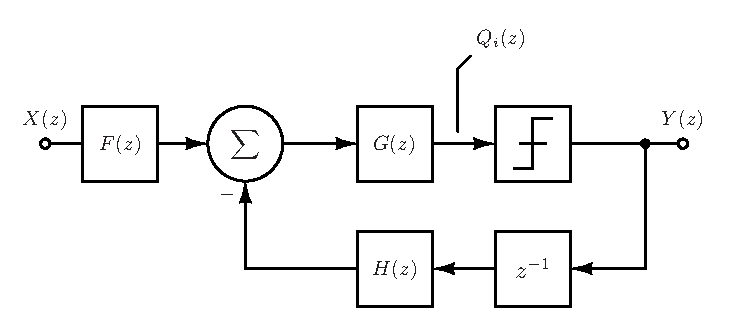
\includegraphics{./final_figures/sim_block_diagram.eps}
 \caption{Discrete-Time Simulation Model}
 \label{fig:dsm_sim_model}
\end{figure}
%-----------------------
From observation of Figure \ref{fig:dsm_sim_model}, the quantizer's input, $Q_i(z)$, can
be
given as
%-----------------------
\begin{equation}\label{eq:quantizer_input_1}
Q_i(z) = G(z)\left(F(z)X(z)-z^{-1}H(z)Y(z)\right)\text{.}
\end{equation}
%-----------------------
Substituting \eqref{eq:block_diagram_to_canonical_F},
\eqref{eq:block_diagram_to_canonical_G}, and 
\eqref{eq:block_diagram_to_canonical_H} into \eqref{eq:quantizer_input_1}, the quantizer
input, $Q_i(z)$, can be expressed as
%-----------------------
\begin{equation}\label{eq:quantizer_input_2}
\begin{split}
 Q_i(z)&
=\left(\frac{F_n(z)}{G_d(z)}\right)X(z)-z^{-1}\left(\frac{H_n(z)}{G_d(z)}\right)Y(z)\\
 & = \left(\frac
{\displaystyle\sum_{k=0}^{N}\alpha_k z^{-k}}
{\displaystyle\sum_{k=0}^{N}\gamma_k z^{-k}}\right)X(z)
-z^{-1}\left(\frac
{\displaystyle\sum_{k=1}^{N}\left(\beta_k-\gamma_k\right)z^{-k}}
{\displaystyle\sum_{k=0}^{N} \gamma_k z^{-k}}\right)Y(z)\\
\end{split}
\end{equation}
%-----------------------
where $\gamma_0=1$. Alternatively, \eqref{eq:quantizer_input_2} can be written
such that
%-----------------------
\begin{equation}\label{eq:quantizer_input_3}
 Q_i(z)\left(\sum_{k=0}^{N} \gamma_k z^{-k}\right) =
\left(\displaystyle\sum_{k=0}^{N}\alpha_k z^{-k}\right)X(z)-
\left(\displaystyle\sum_{k=1}^{N}\left(\beta_k-\gamma_k\right)z^{-k}\right)Y(z)
\end{equation}
%-----------------------
where $\gamma_0=1$. Taking the inverse $z$-transform of
\eqref{eq:quantizer_input_3}, the quantizer
input, $q_i(n)$, can be written as
%-----------------------
\begin{equation}\label{eq:quantizer_input_discrete_time_1}
\sum_{k=0}^{N}\gamma_k q_i(n-k)=
\sum_{k=0}^{N}\alpha_k x(n-k) -
\sum_{k=1}^{N}\left(\beta_k-\gamma_k\right)y(n-k)
\end{equation}
%-----------------------
which implies that
%-----------------------
\begin{equation}\label{eq:quantizer_input_discrete_time_2}
q_i(n)=\sum_{k=0}^{N}\alpha_k x(n-k)-\sum_{k=1}^{N}\left(\beta_k-\gamma_k\right)y(n-k)-
\sum_{k=1}^{N}\gamma_k q_i(n-k).
\end{equation}
%-----------------------
Because a single-bit quantizer is implemented, the discrete-time output, $y(n)$, is
%-----------------------
\begin{equation}\label{eq:dt_dsm_output_discrete_time}
 y(n)=\mathop\text{sgn}\left[q_i(n)\right]
\end{equation}
%-----------------------
where $\mathop\text{sgn}[\cdot]$ is the signum function.

%%%%%%%%%%%%%%%%%%%%%%%%%%%%%%%%%%%%%%%%%%%%%%%%
% Section 4.3.2 - Decimation Filtering
%%%%%%%%%%%%%%%%%%%%%%%%%%%%%%%%%%%%%%%%%%%%%%%%
\subsection{Decimation Filtering}\label{sec:Decimation Filtering}
Consider a \DS modulator that has a sampling frequency, $f_s$,
and an OSR of $M$, which implies that $f_s=M 2f_0$. A \DS modulator's NTF filters the
quantization noise power, $P_{e(n)}$, over the quantizer's operational bandwidth,
$f_{\text{OS}}$, where $f_{\text{OS}}\in\left[-f_s/2,f_s/2\right]$. By bandlimiting the
ADC's digital output, $y(n)$,  to the input's signal's Nyquist frequency, $f_{\text{NY}}$,
where $f_{\text{NY}}\in\left[-f_0,f_0\right]$, the power spectral density of the input
signal is preserved while the quantization noise power contained in the output signal is
significantly decreased.

Ideally, the output signal would be bandlimited by an ideal digital lowpass filter,
referred to as a decimation filter, with a cutoff frequency of $f_s/2M$. However,
practical decimation filters require a finite transition bandwidth. As a 
result, quantization noise power from the transition band will alias into the operational
region. To mitigate the aliasing of quantization noise power, a \DS modulator's sampling
frequency can be increased and its NTF can be designed such that its stopband corner is
increased. For example, consider a 5th order \DS modulator with an equiripple lowpass
filter that has a cutoff frequency of $\pi/32$ and a magnitude response as shown in Figure
\ref{fig:decimation_spec}.
%-----------------------
\begin{figure}[htbp]
 \centering
 \includegraphics[width=0.8\textwidth]{./matlab_figures/decimation_spec.eps}
 \caption{\DS Output Decimation Filter Magnitude Response}
 \label{fig:decimation_spec}
\end{figure}
%-----------------------
After lowpass filtering, the sample rate of the filter's output is much higher than the
output signal's Nyquist rate. As such, the output signal's sampling rate is typically
reduced, or decimated, to a rate near the input signal's Nyquist
rate\cite{oppenheim_discrete-time_1999}\cite{hayes_schaums_1998}. In practice, the
decimation operation is combined with the filter and is referred to as decimation
filtering.

For this thesis, the output of the simulated \DS modulators was bandlimited using a
Parks-McClellan optimal finite impulse response (FIR) lowpass filter. As illustrated
in Figure \ref{fig:decimation_block_diagram}, the \DS modulator's output, $y(n)$, is
lowpass filtered by $H_d(z)$, which was configured with a cutoff
frequency, $f_c=f_s/2M$, a transition bandwidth of $f_s/2M$, a maximum passband
ripple of 0.1 dB, and a minimum stopband attenuation of 200 dB. Subsequent to filtering,
the filter's output signal, $y_f(n)$, was downsampled by a factor of $M/2$.
%-----------------------
\begin{figure}[htbp]
 \centering
 \includegraphics[width=0.8\textwidth]{./final_figures/decimation_block_diagram}
 \caption{\DS Modulator Output Decimation and Filtering Block Diagram}
 \label{fig:decimation_block_diagram}
\end{figure}
%-----------------------

%%%%%%%%%%%%%%%%%%%%%%%%%%%%%%%%%%%%%%%%%%%%%%%%
% Section 4.3.3 - Numerical Analysis
%%%%%%%%%%%%%%%%%%%%%%%%%%%%%%%%%%%%%%%%%%%%%%%%
\subsection{Numerical Analysis}\label{sec:Numerical Analysis}
The SNR or DR of a \DS modulator are typically calculated from the characteristics of
the \DS modulator's output spectrum; that is, the effective resolution of a \DS
modulator can be calculated by using the Discrete Fourier Transform (DFT) or equivalently
a Fast Fourier Transform (FFT) of its output.

In the time domain, the power of the finite length decimated output signal, $y_d(n)$, is
calculated as
%-----------------------
\begin{equation}\label{eq:time_domain_power}
 P_{y_d(n)}=\frac{1}{N}\sum_{k=0}^{N-1}y_d^2(k)
\end{equation}
%-----------------------
Using Parseval's theorem, the average output power, $P_\text{avg}$, of the decimated
output signal, $y_d(n)$, can be written as
%-----------------------
\begin{equation}\label{eq:parseval}
 P_{\text{avg}}=\frac{1}{N}\sum_{k=0}^{N-1}\lvert
y_d(n)\rvert^2=\frac{1}{N^2}\sum_{k=0}^{N-1}
\lvert Y_d(k)\rvert^2
\end{equation}
%-----------------------
where $Y_d(k)$ corresponds to the $k$th element, or bin, of the DFT of
$y_d(n)$. Thus, a \DS modulator's SNR and DR can be determined by calculating
signal and noise power from the \DS modulator's output spectrum. Because the output
signal has been decimated by a 
factor of $M/2$, the post-decimation operational bandwidth is $f_{\text{BW}}$, where
$f_{\text{BW}}\in\left[-f_s/2M,f_s/2M\right]$. Thus, for a $N$-point FFT, the FFT
bins, $\{k\}$, that correspond to the operational bandwidth of the \DS modulator are
$\{k:0\leq k\leq N/4-1\}$ and $\{k:3N/4\leq k\leq N-1\}$ assuming $N$ is even.
Because the output signal is real, $$Y_d(k)=Y_d^*(N-k),$$ and the power can be calculated
using the bins, $\{k:0\leq k\leq N/4-1\}$.

Once the output signal has been decimated and filtered, windowing is
performed to reduce the impact of spectral leakage due to non-coherent sampling
\cite{cerna_harvey_2000}. For this thesis, a normalized Chebyshev window with
a sidelobe suppression of 200 dB was selected. The Chebyshev window was normalized so
that it would not affect the calculated output power spectral density. To illustrate, the 
windowed output signal, $y_w(n)$, can be written as
%-----------------------
\begin{equation}\label{eq:window_output}
 y_w(n) = y_d(n)w_n(n)
\end{equation}
%-----------------------
where $y_d(n)$ corresponds to the filtered and decimated output signal and $w_n(n)$
corresponds to the normalized window function. If $y_d(n)$ and $w_n(n)$ are
uncorrelated, the power of the windowed output signal, $P_{y_w(n)}$, can be written as
%-----------------------
\begin{equation}\label{eq:windowed_output_power}
P_{y_w(n)}=E\left[y_w^2(n)\right]=E\left[y_d^2(n)\right]E\left[w^2_n(n)\right]=P_{y_d(n)}
P_ { w_n(n)}
\end{equation}
%-----------------------
which implies that $P_{y_w(n)}=P_{y_d(n)}$ when $$P_{w_n(n)}=E\left[w^2_n(n)\right]=1.$$
Thus, if a window, $w(n)$, has an average power, $P_{w(n)}$, the normalized window,
$w_n(n)$, is $$w_n(n)=\frac{w(n)}{\displaystyle\sqrt{P_{w(n)}}}$$ so
that 
%-----------------------
\begin{equation}\label{eq:average_window_power}
 E\left[w^2_n(n)\right]=E\left[\frac{w^2(n)}{P_{w(n)}}\right]=\frac{1}{P_{w(n)}}E\left
[w^2(n)\right]=1.
\end{equation}
%-----------------------

Because windows can smear the signal energy into adjacent FFT bins, the signal power,
$P_s$, can be calculated by summing the DFT coefficients within the bounds of
the input signal lobe; that is,
%-----------------------
\begin{equation}\label{eq:signal_power_freq}
 P_s=\frac{2}{N^2}\sum_{k=K_1}^{K_2}\left\lvert
Y_w(k)\right\rvert^2, 
\end{equation}
%-----------------------
where $K_1$ and $K_2$ correspond to the leading and trailing FFT bins of the input
signal lobe and $N$ is the length of the DFT.
Similarly, the noise power, $P_n$, can be calculated from the DFT coefficients. In
particular, the average noise power,
$P_{n,a}$, can be expressed as
%-----------------------
\begin{equation}\label{eq:noise_power_freq_1}
P_{n,a} =\frac{2}{N^2}\left(\sum_{k=0}^{K_1-1}\left\lvert
Y_w(k)\right\rvert^2 + \sum_{k=K_2+1}^{N/4-1} \left\lvert
Y_w(k)\right\rvert^2+(K_2-K_1)\lvert\hat{Y}_w^2(k)\rvert\right)
\end{equation}
%-----------------------
where $K_1$ and $K_2$ correspond to the leading and trailing FFT bins of the
fundamental signal lobe, $\hat{Y}_w$ is the estimated average noise magnitude in the
fundamental signal lobe's FFT bins, and $N$ is the length of the DFT. Observe that for
narrow band input signals, that is, for $$K_2-K_1\ll N/4-1,$$ the average noise power can
be approximated as 
%-----------------------
\begin{equation}\label{eq:noise_power_freq_2}
P_{n,a} \approx \frac{2}{N^2}\left(\sum_{k=0}^{K_1-1}\left\lvert
Y_w(k)\right\rvert^2 + \sum_{k=K_2+1}^{N/4-1} \left\lvert
Y_w(k)\right\rvert^2\right)
\end{equation}
%-----------------------
Thus, the SNR expressed in decibels can be calculated by substituting
\eqref{eq:signal_power_freq} and \eqref{eq:noise_power_freq_2} into \eqref{eq:SNR} such
that
%-----------------------
\begin{equation}\label{eq:SNR_freq}
 \text{SNR}_\text{dB}=10\log\left(\frac{P_s}{P_{n,a}}\right)=10\log\left(\frac
{
\displaystyle\sum_{k=K_1}^{K_2}\left\lvert
Y_w(k)\right\rvert^2
}
{
\displaystyle\sum_{k=0}^{K_1-1}\left\lvert Y_w(k)\right\rvert^2 +
\sum_{k=K_2+1}^{N/4-1} \left\lvert Y_w(k)\right\rvert^2
}\right)
\end{equation}
%-----------------------

Recall that DR is defined as the ratio of the maximum to the minimum detectable
signal levels. Because the minimum detectable signal level is determined by the peak
noise floor magnitude, the DR can be defined numerically as the ratio of the maximum
signal power to a uniform noise floor which is equal in magnitude to the observed peak
noise floor magnitude. As such, if $y_{d,e}(n)$ is the noise component of the decimated
output signal, $y_d(n)$, the observed peak noise floor, $N_p$, is defined as
%-----------------------
\begin{equation}\label{eq:max_noise_floor}
N_p=\max\langle\lvert Y_{d,e}(k)\rvert\rangle
\end{equation}
%-----------------------
where $Y_{d,e}(k)$ is the DFT of $y_{d,e}(n)$. Thus, the average power, $P_{n,p}$, for a
uniform noise floor with a magnitude equal to the observed peak noise floor value, $N_p$,
is given as
%-----------------------
\begin{equation}\label{eq:peak_avg_power}
P_{n,p}=\frac{2}{N^2}\sum_{k=0}^{N/4-1}N_p=\frac{2}{4N}N_p =\frac{N_p}{2N}.
\end{equation}
%-----------------------
Thus, the DR expressed in dB can be calculated by substituting
\eqref{eq:signal_power_freq} and \eqref{eq:peak_avg_power} into \eqref{eq:SNR} such that
%-----------------------
\begin{equation}\label{eq:DR_freq}
\begin{split}
\text{DR}_{\text{dB}}& =10\log\left(\frac{P_s}{P_{n,p}}\right)\\
& =10\log\left(\frac
{
\frac{2}{N^2}\displaystyle\sum_{k=K_1}^{K_2}\left\lvert
Y_w(k)\right\rvert^2
}
{
\displaystyle\frac{N_p}{2N}
}\right)\\
& = 10\log\left(\frac{4}{N_pN}\sum_{k=K_1}^{K_2}\lvert Y_w(k)\rvert^2\right)
\end{split}
\end{equation}
%-----------------------
where $N_p$ corresponds to the largest noise magnitude contained in the
output spectrum.

%%%%%%%%%%%%%%%%%%%%%%%%%%%%%%%%%%%%%%%%%%%%%%%%
% Section 4.4 - Results and Observations
%%%%%%%%%%%%%%%%%%%%%%%%%%%%%%%%%%%%%%%%%%%%%%%%
\section{Results and Observations}\label{sec:Results and Observations}

In this section, three \DS design methods are compared. Specifically, the methods are the
Delta Sigma (DelSig) Toolbox for MATLAB\textsuperscript{\textregistered}, the Chebyshev
filter, and the HOG algorithm based design method. The DelSig method claims to maximize
the SNR by uniformly distributing the system function zeros over the passband and then
optimizing the pole locations. Chebyshev filters generate equiripple stopbands and
maximally flat passbands and are typically used to maximize DR. The HOG algorithm based
design method maximizes a weighted combination of SNR, DR, and a 1-norm approximation of
the passband as described in Section \ref{sec:DSM Design Objective Functions}. Each method
is used to design \DS modulators over a range of OSRs and filter orders. A detailed
comparison of 5th and 6th order systems is presented followed by an inclusive summary of
all design cases.

Figure \ref{fig:NTF_comparison_5} shows a comparison of the NTF magnitude responses for
the various design techniques for a 5th order \DS modulator with an OSR of 32. As
illustrated, the peak and average stopband spectrum for NTFs derived by the HOG algorithm 
is lower than both the classical Chebyshev based NTF and the DelSig toolbox's NTF.
Additionally, note that the shape of the stopband frequency response reflects the
optimization for a weighted combination of SNR and DR.
%-----------------------
\begin{figure}[htbp]
	\centering
	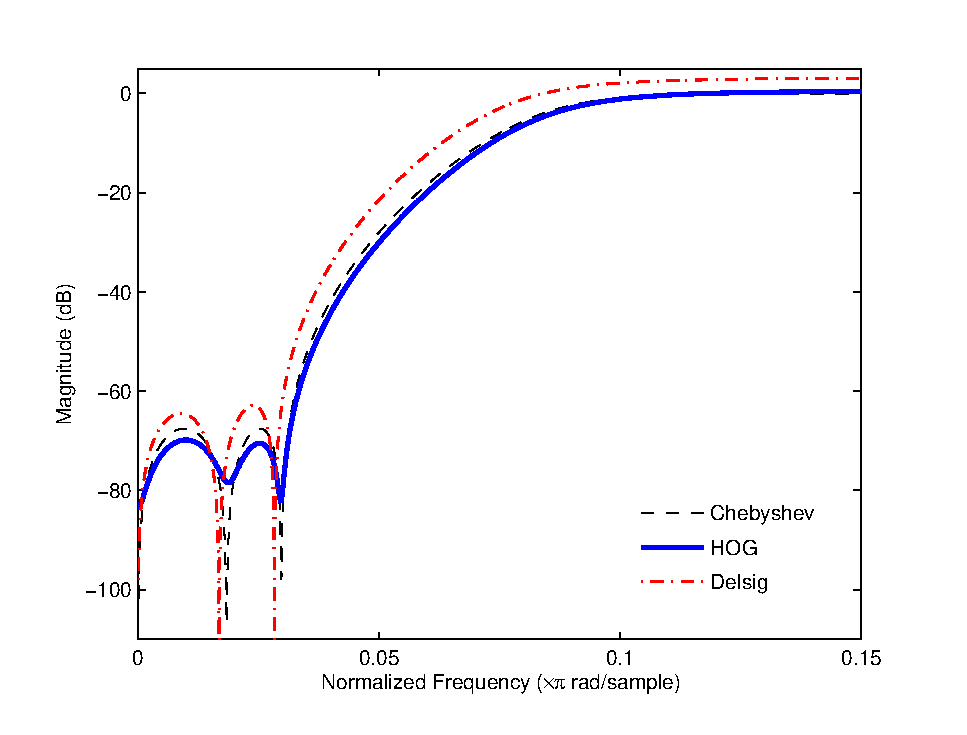
\includegraphics[width=0.75\textwidth]
{./matlab_figures/5th_order_NTFs.eps}
	\caption[]
{5th Order NTF Comparison\\
OSR: 32 - BW: $\pi$/OSR (rad/sample)}
	\label{fig:NTF_comparison_5}
\end{figure}
%-----------------------

Figure \ref{fig:STF_comparison_5} shows a comparison of the STF magnitude responses for
the corresponding NTFs  illustrated in Figure \ref{fig:NTF_comparison_5}.
%-----------------------
\begin{figure}[htbp]
	\centering
	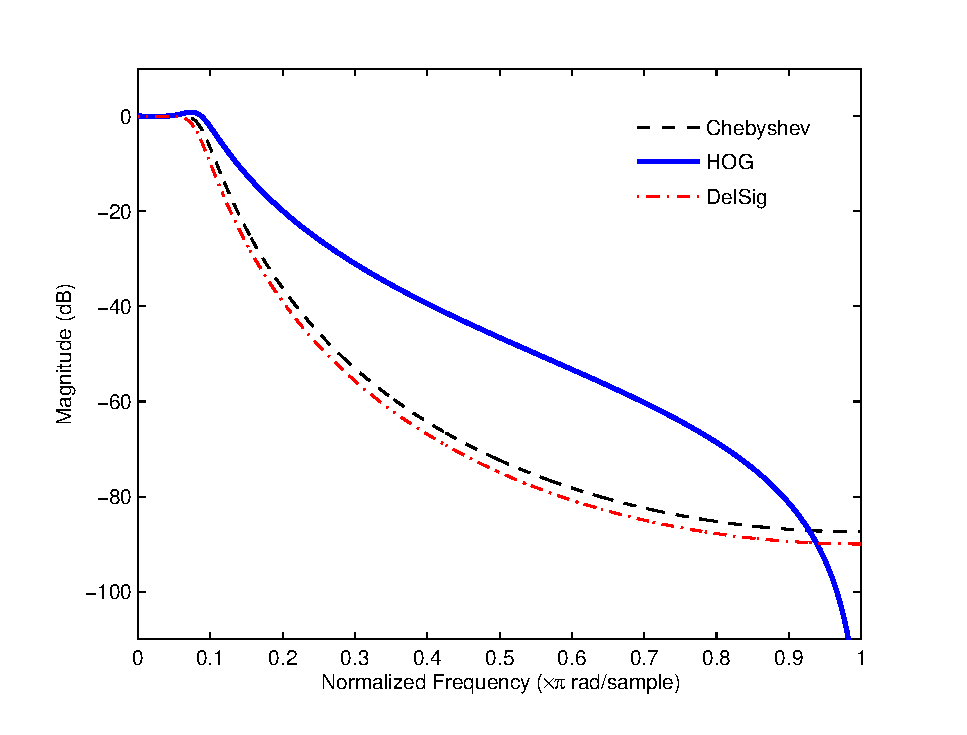
\includegraphics[width=0.75\textwidth]
{./matlab_figures/5th_order_STFs.eps}
	\caption[]
{5th Order STF Comparison\\
OSR: 32 - BW: $\pi$/OSR (rad/sample)}
	\label{fig:STF_comparison_5}
\end{figure}
%-----------------------
The STF designed with the HOG algorithm, shown in Figure
\ref{fig:STF_comparison_5}, was optimized as described in Section
\ref{sec:STF_Objective_Function}.

Figure \ref{fig:PSD_comparison_5} illustrates the output spectra for the 5th order
\DS modulator that uses the STFs and NTFs shown in Figures \ref{fig:NTF_comparison_5} and
\ref{fig:STF_comparison_5}.
%-----------------------
\begin{figure}[htbp]
	\centering
	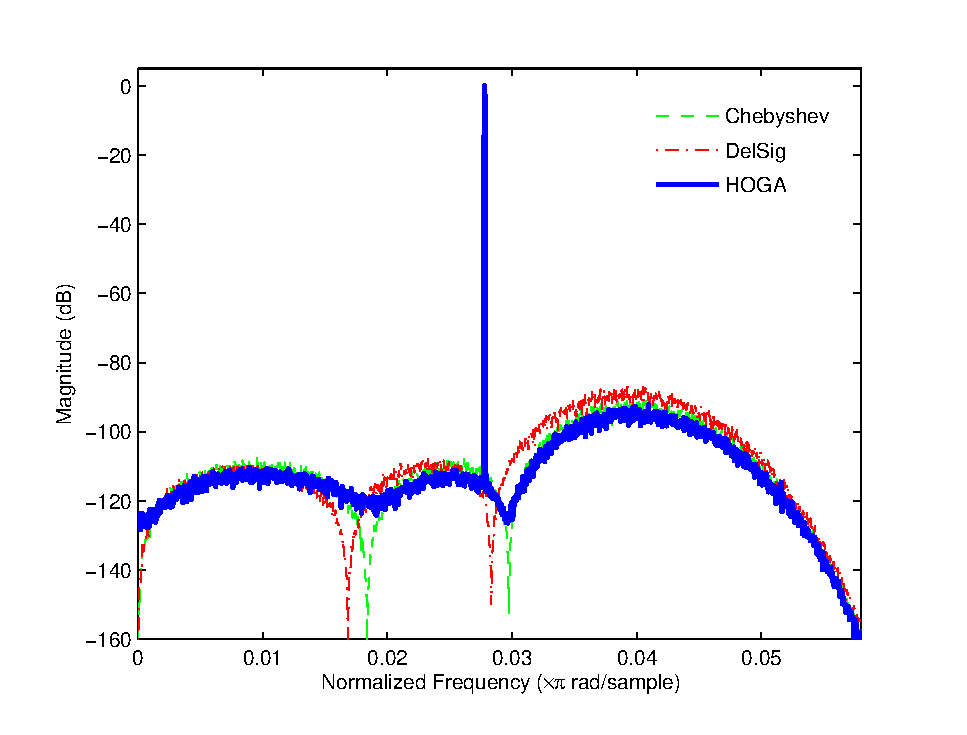
\includegraphics[width=0.75\textwidth]
{./matlab_figures/5th_order_spectra.eps}
	\captionsetup{justification=centering}
	\caption[]
{5th Order Output PSD Comparison\\
OSR: 32 - BW: $\pi$/OSR (rad/sample)- FFT Length: 8192}
	\label{fig:PSD_comparison_5}
\end{figure}
%----------------------- 
From the spectra shown in Figure \ref{fig:PSD_comparison_5}, the calculated SNRs and DRs
for the DelSig Toolbox, Chebyshev filter, and HOG algorithm based design method are
summarized in Table \ref{tbl:results_comparison_5}. Based on the SNR and DR values, it can
be seen that the HOG algorithm based design produces NTFs and STFs which achieve a higher
effective resolution than both the DelSig method and the Chebyshev filter.
%----------------------------
\begin{table}[htbp]
 \begin{center}
 \caption[5th Order \DS Modulator Results]{5th Order \DS Modulators: Calculated SNRs and
DRs}
 \label{tbl:results_comparison_5}
 \begin{tabular}{ l c c }\toprule
 \textbf{Design Method}  & \textbf{SNR$_\text{dB}$} & \textbf{DR$_\text{dB}$} \\ \midrule
        DelSig Toolbox   &     83       &     66      \\
        Chebyshev Filter &     81       &     72      \\
        HOG Algorithm    &     87       &     76      \\ \bottomrule
\end{tabular}
\end{center}
\end{table}
%----------------------------

Figure \ref{fig:NTF_comparison_6} shows a comparison of the NTF magnitude responses for
the various design techniques for a 6th order \DS modulator with an OSR of 32. Again, the
peak and average stopband spectrum for NTFs determined by the HOG algorithm is lower than
both the classical Chebyshev based NTF and the Delta Sigma toolbox's NTF and has a
stopband shape which reflects the optimization for a weighted combination of SNR and DR. 
%-----------------------
\begin{figure}[htbp]
	\centering
	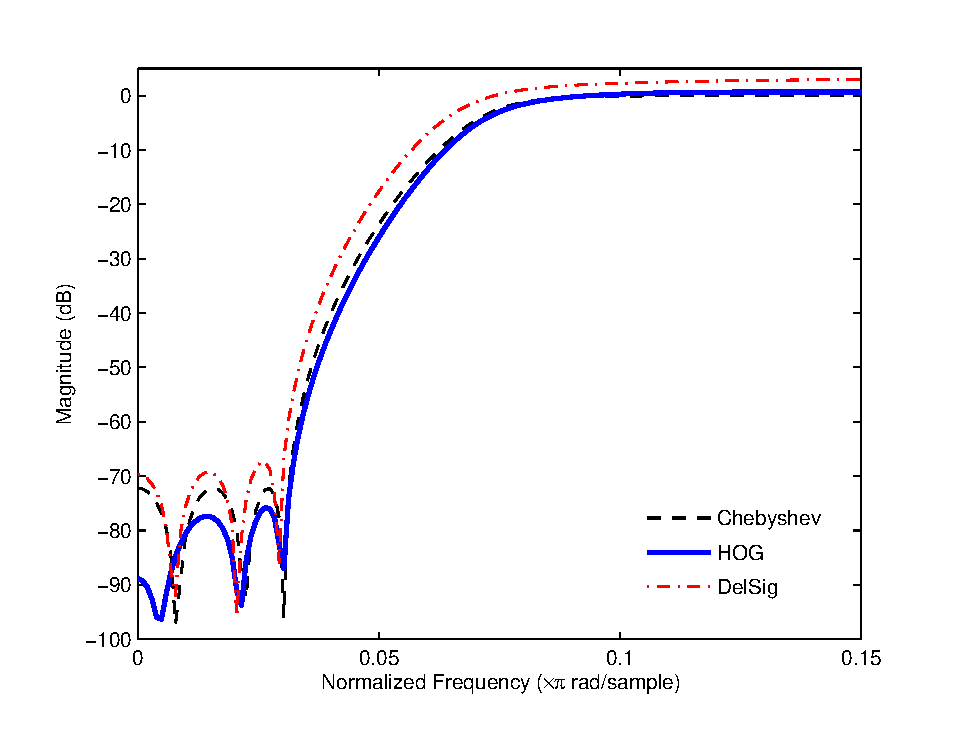
\includegraphics[width=0.75\textwidth]
{./matlab_figures/6th_order_NTFs.eps}
	\caption[]
{6th Order NTF Comparison\\
OSR: 32 - BW: $\pi$/OSR (rad/sample)}
	\label{fig:NTF_comparison_6}
\end{figure}
%-----------------------

Figure \ref{fig:STF_comparison_6} shows a comparison of the STF
magnitude responses for the corresponding NTFs  illustrated in Figure
\ref{fig:NTF_comparison_6}.
%-----------------------
\begin{figure}[htbp]
	\centering
	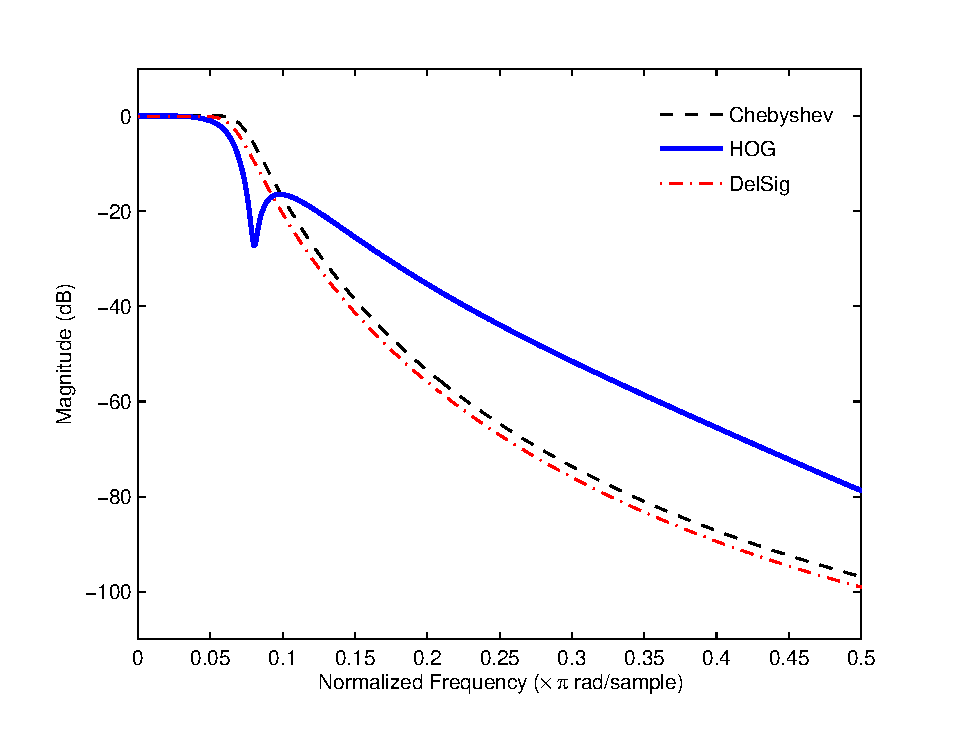
\includegraphics[width=0.75\textwidth]
{./matlab_figures/6th_order_STFs.eps}
	\caption[]
{6th Order STF Comparison\\
OSR: 32 - BW: $\pi$/OSR (rad/sample)}
	\label{fig:STF_comparison_6}
\end{figure}
%-----------------------
Again, the passband of the STF designed with the HOG algorithm, shown in Figure
\ref{fig:STF_comparison_6}, was optimized as described in Section
\ref{sec:STF_Objective_Function}.

Figure \ref{fig:PSD_comparison_6} illustrates the output spectra for the 6th order
\DS modulator that uses the STFs and NTFs shown in Figures \ref{fig:NTF_comparison_6} and
\ref{fig:STF_comparison_6}.
%-----------------------
\begin{figure}[htbp]
	\centering
	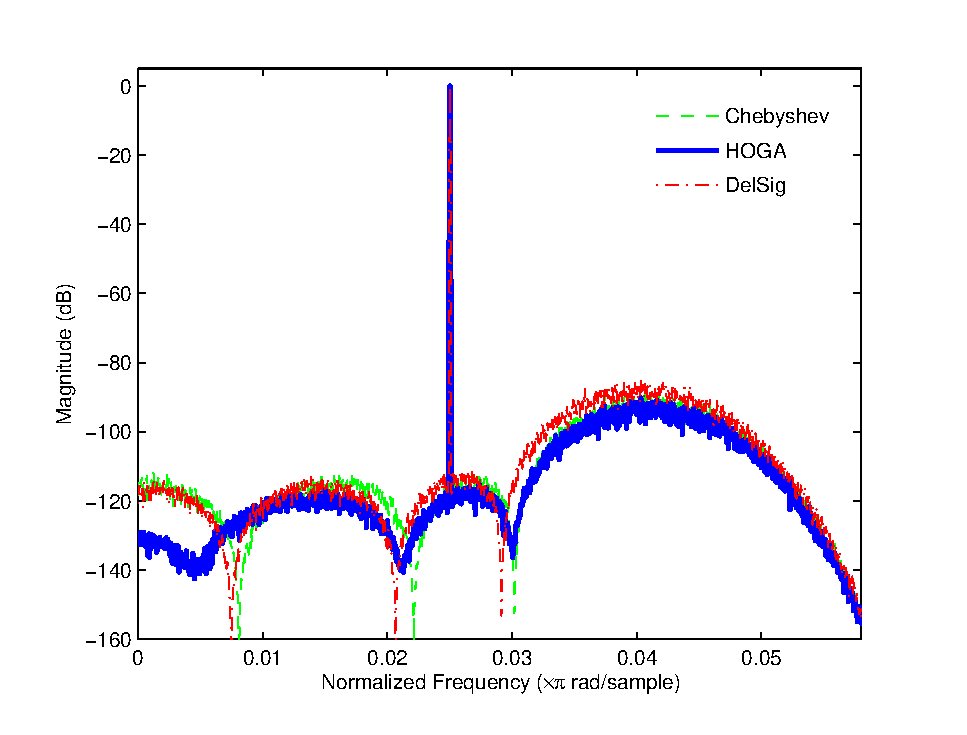
\includegraphics[width=0.75\textwidth]
{./matlab_figures/6th_order_spectra.eps}
	\captionsetup{justification=centering}
	\caption[]
{6th Order Output PSD Comparison\\
OSR: 32 - BW: $\pi$/OSR (rad/sample) - FFT Length: 8192}
	\label{fig:PSD_comparison_6}
\end{figure} 
%-----------------------
From the spectra shown in Figure \ref{fig:PSD_comparison_6}, the calculated SNRs and DRs
for the DelSig Toolbox, Chebyshev filter, and HOG algorithm based design method are
summarized in Table \ref{tbl:results_comparison_6}. Based on the SNR and DR values, it can
be seen that the HOG algorithm based design produces NTFs and STFs which achieve a higher
effective resolution than both the DelSig method and the Chebyshev filter.
%----------------------------
\begin{table}[htbp]
 \begin{center}
 \caption[6th Order \DS Modulator Results]{6th Order \DS Modulators: Calculated SNRs and
DRs}
 \label{tbl:results_comparison_6}
 \begin{tabular}{ l c c }\toprule
 \textbf{Design Method}  & \textbf{SNR$_\text{dB}$} & \textbf{DR$_\text{dB}$} \\ \midrule
        DelSig Toolbox   &     88       &     74      \\
        Chebyshev Filter &     87       &     77      \\
        HOG Algorithm    &     91       &     80      \\ \bottomrule
\end{tabular}
\end{center}
\end{table}
%----------------------------

Several \DS modulators were designed using the methods previously described. Figures
\ref{fig:SNR_DR_32_comparison}, \ref{fig:SNR_DR_64_comparison}, and
\ref{fig:SNR_DR_128_comparison} summarize the resulting SNRs and DRs as a function of
filter order for OSRs of 32, 64, and 128, respectively. Note that the HOG algorithm based
method provides improved SNR and DR over both the classical and contemporary design
methods.
%-----------------------
\begin{figure}[htbp]
	\centering
	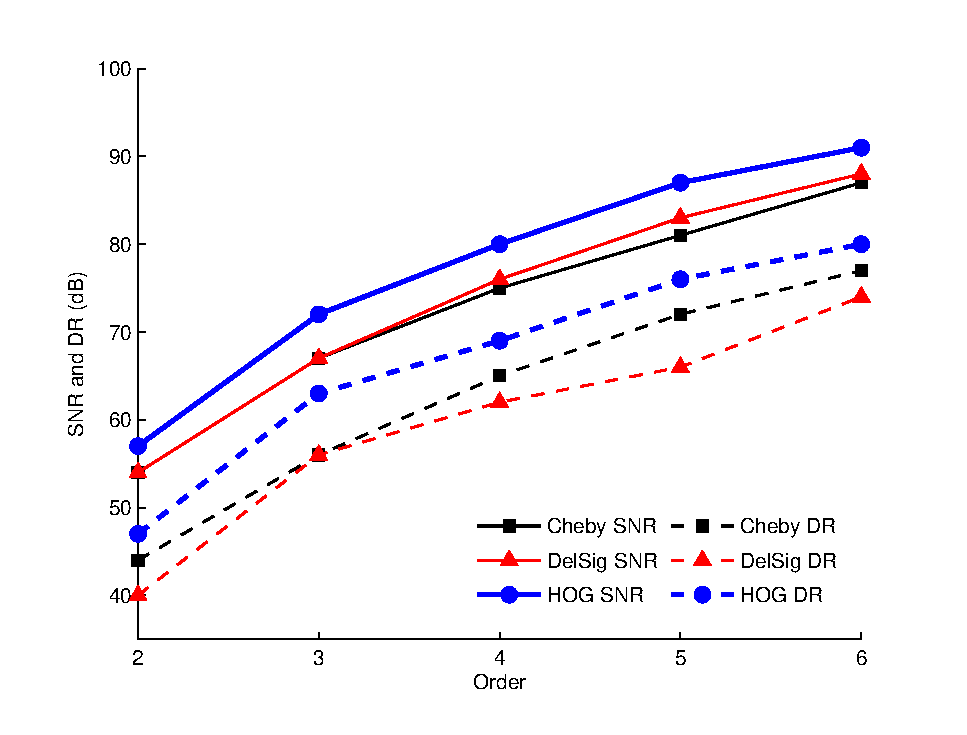
\includegraphics[width=0.75\textwidth]{./matlab_figures/OSR_32_chart.eps}
	\caption{SNR and DR Results with $\text{OSR}=32$}
	\label{fig:SNR_DR_32_comparison}
\end{figure}
%-----------------------
\begin{figure}[htbp]
	\centering
	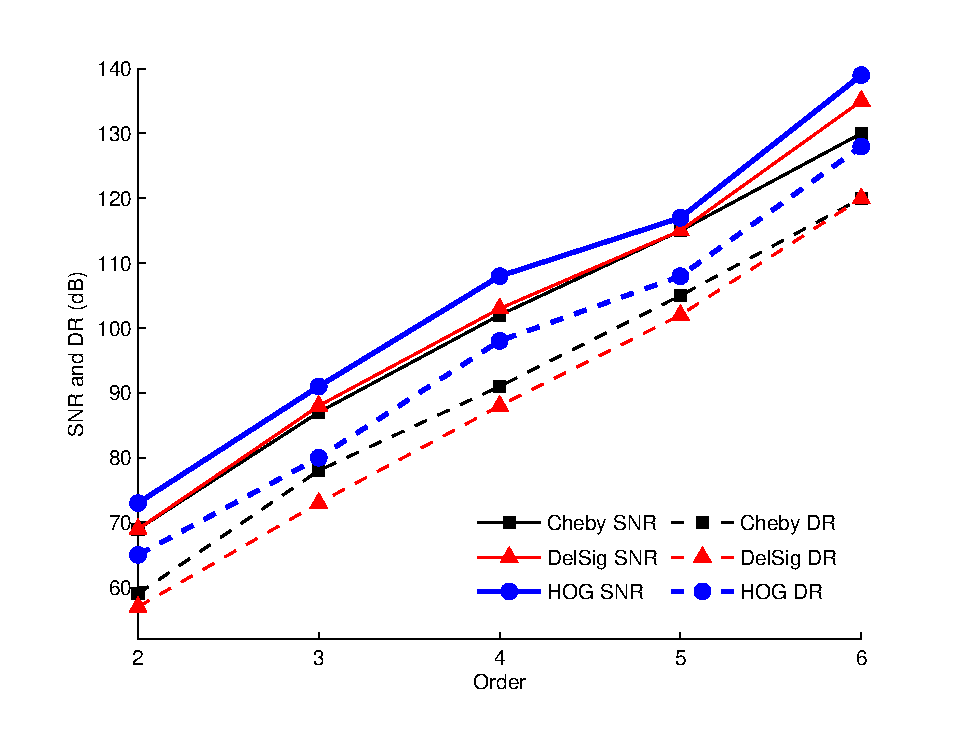
\includegraphics[width=0.75\textwidth]{./matlab_figures/OSR_64_chart.eps}
	\caption{SNR and DR Results with $\text{OSR}=64$}
	\label{fig:SNR_DR_64_comparison}
\end{figure}
%-----------------------
\begin{figure}[htbp]
	\centering
	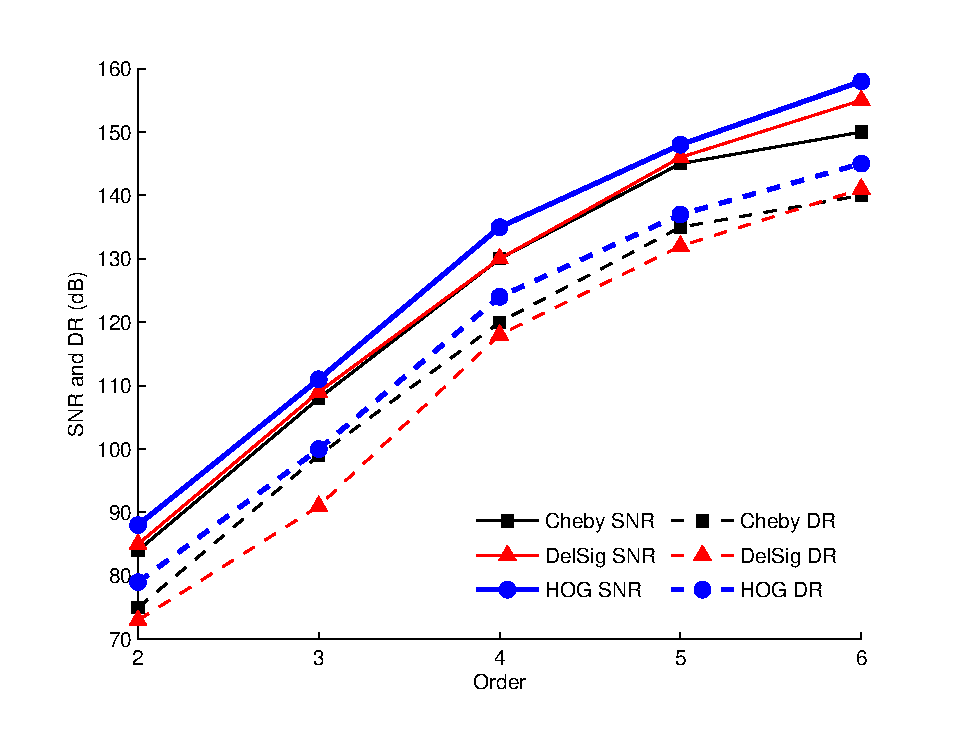
\includegraphics[width=0.75\textwidth]{./matlab_figures/OSR_128_chart.eps}
	\caption{SNR and DR Results with $\text{OSR}=128$}
	\label{fig:SNR_DR_128_comparison}
\end{figure}
%-----------------------

% CHAPTER 5: CONCLUSION
\chapter{Conclusion}
\label{ch:Conclusion}
\input{conclusion}

% BIBLIOGRAPHY
\singlespacebib
\bibliography{new_bib}
\bibliographystyle{plain}

% VITA
\newpage
\addcontentsline{toc}{chapter}{VITA} 
\thesisauthorvita

\end{document}